% Options for packages loaded elsewhere
\PassOptionsToPackage{unicode}{hyperref}
\PassOptionsToPackage{hyphens}{url}
%
\documentclass[
]{report}
\usepackage{amsmath,amssymb}
\usepackage{lmodern}
\usepackage{iftex}
\ifPDFTeX
  \usepackage[T1]{fontenc}
  \usepackage[utf8]{inputenc}
  \usepackage{textcomp} % provide euro and other symbols
\else % if luatex or xetex
  \usepackage{unicode-math}
  \defaultfontfeatures{Scale=MatchLowercase}
  \defaultfontfeatures[\rmfamily]{Ligatures=TeX,Scale=1}
\fi
% Use upquote if available, for straight quotes in verbatim environments
\IfFileExists{upquote.sty}{\usepackage{upquote}}{}
\IfFileExists{microtype.sty}{% use microtype if available
  \usepackage[]{microtype}
  \UseMicrotypeSet[protrusion]{basicmath} % disable protrusion for tt fonts
}{}
\makeatletter
\@ifundefined{KOMAClassName}{% if non-KOMA class
  \IfFileExists{parskip.sty}{%
    \usepackage{parskip}
  }{% else
    \setlength{\parindent}{0pt}
    \setlength{\parskip}{6pt plus 2pt minus 1pt}}
}{% if KOMA class
  \KOMAoptions{parskip=half}}
\makeatother
\usepackage{xcolor}
\usepackage{color}
\usepackage{fancyvrb}
\newcommand{\VerbBar}{|}
\newcommand{\VERB}{\Verb[commandchars=\\\{\}]}
\DefineVerbatimEnvironment{Highlighting}{Verbatim}{commandchars=\\\{\}}
% Add ',fontsize=\small' for more characters per line
\usepackage{framed}
\definecolor{shadecolor}{RGB}{248,248,248}
\newenvironment{Shaded}{\begin{snugshade}}{\end{snugshade}}
\newcommand{\AlertTok}[1]{\textcolor[rgb]{0.94,0.16,0.16}{#1}}
\newcommand{\AnnotationTok}[1]{\textcolor[rgb]{0.56,0.35,0.01}{\textbf{\textit{#1}}}}
\newcommand{\AttributeTok}[1]{\textcolor[rgb]{0.77,0.63,0.00}{#1}}
\newcommand{\BaseNTok}[1]{\textcolor[rgb]{0.00,0.00,0.81}{#1}}
\newcommand{\BuiltInTok}[1]{#1}
\newcommand{\CharTok}[1]{\textcolor[rgb]{0.31,0.60,0.02}{#1}}
\newcommand{\CommentTok}[1]{\textcolor[rgb]{0.56,0.35,0.01}{\textit{#1}}}
\newcommand{\CommentVarTok}[1]{\textcolor[rgb]{0.56,0.35,0.01}{\textbf{\textit{#1}}}}
\newcommand{\ConstantTok}[1]{\textcolor[rgb]{0.00,0.00,0.00}{#1}}
\newcommand{\ControlFlowTok}[1]{\textcolor[rgb]{0.13,0.29,0.53}{\textbf{#1}}}
\newcommand{\DataTypeTok}[1]{\textcolor[rgb]{0.13,0.29,0.53}{#1}}
\newcommand{\DecValTok}[1]{\textcolor[rgb]{0.00,0.00,0.81}{#1}}
\newcommand{\DocumentationTok}[1]{\textcolor[rgb]{0.56,0.35,0.01}{\textbf{\textit{#1}}}}
\newcommand{\ErrorTok}[1]{\textcolor[rgb]{0.64,0.00,0.00}{\textbf{#1}}}
\newcommand{\ExtensionTok}[1]{#1}
\newcommand{\FloatTok}[1]{\textcolor[rgb]{0.00,0.00,0.81}{#1}}
\newcommand{\FunctionTok}[1]{\textcolor[rgb]{0.00,0.00,0.00}{#1}}
\newcommand{\ImportTok}[1]{#1}
\newcommand{\InformationTok}[1]{\textcolor[rgb]{0.56,0.35,0.01}{\textbf{\textit{#1}}}}
\newcommand{\KeywordTok}[1]{\textcolor[rgb]{0.13,0.29,0.53}{\textbf{#1}}}
\newcommand{\NormalTok}[1]{#1}
\newcommand{\OperatorTok}[1]{\textcolor[rgb]{0.81,0.36,0.00}{\textbf{#1}}}
\newcommand{\OtherTok}[1]{\textcolor[rgb]{0.56,0.35,0.01}{#1}}
\newcommand{\PreprocessorTok}[1]{\textcolor[rgb]{0.56,0.35,0.01}{\textit{#1}}}
\newcommand{\RegionMarkerTok}[1]{#1}
\newcommand{\SpecialCharTok}[1]{\textcolor[rgb]{0.00,0.00,0.00}{#1}}
\newcommand{\SpecialStringTok}[1]{\textcolor[rgb]{0.31,0.60,0.02}{#1}}
\newcommand{\StringTok}[1]{\textcolor[rgb]{0.31,0.60,0.02}{#1}}
\newcommand{\VariableTok}[1]{\textcolor[rgb]{0.00,0.00,0.00}{#1}}
\newcommand{\VerbatimStringTok}[1]{\textcolor[rgb]{0.31,0.60,0.02}{#1}}
\newcommand{\WarningTok}[1]{\textcolor[rgb]{0.56,0.35,0.01}{\textbf{\textit{#1}}}}
\usepackage{longtable,booktabs,array}
\usepackage{calc} % for calculating minipage widths
% Correct order of tables after \paragraph or \subparagraph
\usepackage{etoolbox}
\makeatletter
\patchcmd\longtable{\par}{\if@noskipsec\mbox{}\fi\par}{}{}
\makeatother
% Allow footnotes in longtable head/foot
\IfFileExists{footnotehyper.sty}{\usepackage{footnotehyper}}{\usepackage{footnote}}
\makesavenoteenv{longtable}
\usepackage{graphicx}
\makeatletter
\def\maxwidth{\ifdim\Gin@nat@width>\linewidth\linewidth\else\Gin@nat@width\fi}
\def\maxheight{\ifdim\Gin@nat@height>\textheight\textheight\else\Gin@nat@height\fi}
\makeatother
% Scale images if necessary, so that they will not overflow the page
% margins by default, and it is still possible to overwrite the defaults
% using explicit options in \includegraphics[width, height, ...]{}
\setkeys{Gin}{width=\maxwidth,height=\maxheight,keepaspectratio}
% Set default figure placement to htbp
\makeatletter
\def\fps@figure{htbp}
\makeatother
\setlength{\emergencystretch}{3em} % prevent overfull lines
\providecommand{\tightlist}{%
  \setlength{\itemsep}{0pt}\setlength{\parskip}{0pt}}
\setcounter{secnumdepth}{5}
\newlength{\cslhangindent}
\setlength{\cslhangindent}{1.5em}
\newlength{\csllabelwidth}
\setlength{\csllabelwidth}{3em}
\newlength{\cslentryspacingunit} % times entry-spacing
\setlength{\cslentryspacingunit}{\parskip}
\newenvironment{CSLReferences}[2] % #1 hanging-ident, #2 entry spacing
 {% don't indent paragraphs
  \setlength{\parindent}{0pt}
  % turn on hanging indent if param 1 is 1
  \ifodd #1
  \let\oldpar\par
  \def\par{\hangindent=\cslhangindent\oldpar}
  \fi
  % set entry spacing
  \setlength{\parskip}{#2\cslentryspacingunit}
 }%
 {}
\usepackage{calc}
\newcommand{\CSLBlock}[1]{#1\hfill\break}
\newcommand{\CSLLeftMargin}[1]{\parbox[t]{\csllabelwidth}{#1}}
\newcommand{\CSLRightInline}[1]{\parbox[t]{\linewidth - \csllabelwidth}{#1}\break}
\newcommand{\CSLIndent}[1]{\hspace{\cslhangindent}#1}
\usepackage{booktabs}
\usepackage{geometry}
\usepackage[none]{hyphenat}
\usepackage{titlesec}
\usepackage{longtable}
\usepackage{xcolor}
\usepackage{setspace}
\usepackage{pdfpages}

\pagestyle{plain}

%%%% Set margins
\setlength{\topmargin}{-1cm}
\addtolength{\evensidemargin}{-1cm}
\addtolength{\oddsidemargin}{-1cm}
\addtolength{\textheight}{3cm}
\addtolength{\textwidth}{2cm}

% Spacing for reading guides
\newcommand{\rgs}{\vspace{12pt}} % Vertical space
\newcommand{\rgi}{\hspace{24pt}}  % Indent

\newcommand\latexcode[1]{#1}

% Format chapter titles and spacing
\renewcommand*{\chaptername}{Week}

\titleformat{\chapter}[display]
{\bfseries\Large}
{\filleft\MakeUppercase{\chaptertitlename} \Huge\thechapter}
{3ex}
{\titlerule
\vspace{1.5ex}%
\filright}
[\vspace{1.5ex}%
\titlerule]
\titlespacing*{\chapter}{0pt}{-40pt}{20pt}
\ifLuaTeX
  \usepackage{selnolig}  % disable illegal ligatures
\fi
\IfFileExists{bookmark.sty}{\usepackage{bookmark}}{\usepackage{hyperref}}
\IfFileExists{xurl.sty}{\usepackage{xurl}}{} % add URL line breaks if available
\urlstyle{same} % disable monospaced font for URLs
\hypersetup{
  hidelinks,
  pdfcreator={LaTeX via pandoc}}

\title{\textbf{STAT 216 Coursepack}\\
\strut \\
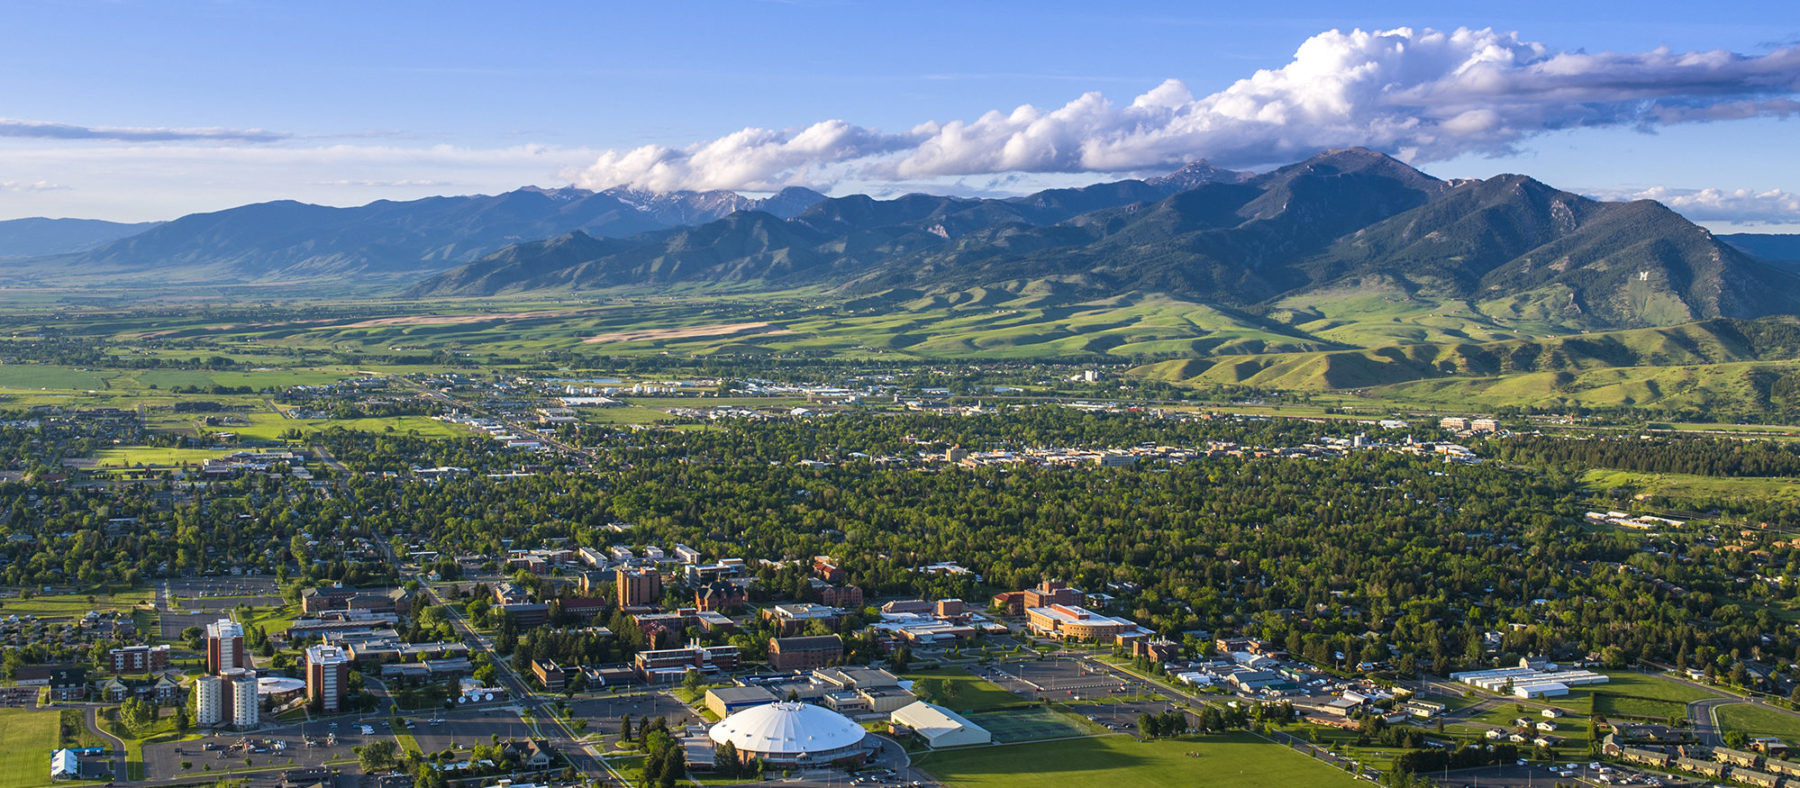
\includegraphics[width=5in,height=\textheight]{images/msu-campus.jpg}}
\usepackage{etoolbox}
\makeatletter
\providecommand{\subtitle}[1]{% add subtitle to \maketitle
  \apptocmd{\@title}{\par {\large #1 \par}}{}{}
}
\makeatother
\subtitle{Spring 2023\\
Montana State University}
\author{Melinda Yager\\
Jade Schmidt\\
Stacey Hancock}
\date{}

\begin{document}
\maketitle

\newpage
\thispagestyle{empty}

This resource was developed by Melinda Yager, Jade Schmidt, and Stacey Hancock in 2021 to accompany the online textbook: Carnegie, N., Hancock, S., Meyer, E., Schmidt, J., and Yager, M. (2021). \emph{Montana State Introductory Statistics with R}. Montana State University. \url{https://mtstateintrostats.github.io/IntroStatTextbook/}.

This resource is released under a \href{https://creativecommons.org/licenses/by-nc-sa/4.0/}{Creative Commons BY-NC-SA 4.0} license unless otherwise noted.

\setcounter{tocdepth}{1}
\addtocontents{toc}{\protect\thispagestyle{empty}}
\tableofcontents
\thispagestyle{empty}

\newpage
\setcounter{page}{1}

\hypertarget{preface}{%
\chapter*{Preface}\label{preface}}
\addcontentsline{toc}{chapter}{Preface}

This coursepack accompanies the textbook for STAT 216: Introduction to Statistics at Montana State University, which can be found at \url{https://mtstateintrostats.github.io/IntroStatTextbook/}. The syllabus for the course (including the course calendar), data sets, and links to D2L Brightspace, Gradescope, and the MSU RStudio server can be found on the course webpage: \url{https://math.montana.edu/courses/s216/}.
Videos assigned in the course calendar and other notes and review materials are linked in D2L.

Each of the activities in this workbook is designed to target specific learning outcomes of the course, giving you practice with important statistical concepts in a group setting with instructor guidance. In addition to the in-class activities for the course, the coursepack includes reading guides to aid in taking notes while you complete the required readings and videos. Bring this workbook with you to class each class period, and take notes in the workbook as you would your own notes. A well-written completed workbook will provide an optimal study guide for exams!

The activities and labs in this coursepack will be completed during class time. Parts of each lab will be turned in on Gradescope. To aid in your understanding, read through the introduction for each activity before attending class each day.

STAT 216 is a 3-credit in-person course. In our experience, it takes six to nine hours per week outside of class to achieve a good grade in this class. By ``good'' we mean at least a C because a grade of D or below does not count toward fulfilling degree requirements. Many of you set your goals higher than just getting a C, and we fully support that. You need roughly nine hours per week to review past activities, read feedback on previous assignments, complete current assignments, and prepare for the next day's class. The following will give you an idea of what a typical week in the life of a STAT 216 student looks like.

\begin{itemize}
\tightlist
\item
  \emph{Prior to class meeting}:

  \begin{itemize}
  \tightlist
  \item
    Read assigned sections of the textbook, using the provided reading guides to take notes on the material.
  \item
    Watch assigned videos on that week's content, pausing to take notes and answer video quiz questions.
  \item
    Read through the introduction to the day's in-class activity.
  \item
    Read through the week's homework assignment and note any questions you may have on the content.
  \end{itemize}
\item
  \emph{During class meeting}:

  \begin{itemize}
  \tightlist
  \item
    Work through the in-class activity or weekly lab with your classmates and instructor, taking detailed notes on your answers to each question in the activity.
  \end{itemize}
\item
  \emph{After class meeting}:

  \begin{itemize}
  \tightlist
  \item
    Complete any parts of the activity you did not complete in class.
  \item
    Review the activity solutions in the Math and Stat Center, and take notes on key points.
  \item
    Finish watching any remaining assigned videos or readings for the week.
  \item
    Complete the week's homework assignment.
  \end{itemize}
\end{itemize}

\nocite{*}

\hypertarget{spring-2023-calendar-of-in-class-activities}{%
\chapter*{Spring 2023 Calendar of In-Class Activities}\label{spring-2023-calendar-of-in-class-activities}}
\addcontentsline{toc}{chapter}{Spring 2023 Calendar of In-Class Activities}

This calendar only lists the in-class activities, RStudio labs and exams each week. For required readings and videos as well as due dates for assignments, refer to the calendar at:\\
\url{https://mtstateintrostats.github.io/Syllabus/\#Course_calendar}

\begin{longtable}{|l|l|l|l|p{.55\textwidth}|}
\hline
\textbf{Week}& \textbf{Day}& \textbf{Date}& \textbf{Activity} \\ \hline
\endhead

1& W& 1/18& Intro to Data \\*
1& F& 1/20& Week 1 Lab \\ \hline
2& M& 1/23& American Indian Address Part A \\*
2& W& 1/25& American Indian Address Part B \\* 
2& F& 1/27& Week 2 Lab \\ \hline
3& M& 1/30& Myopia and Nightlights\\*
3& W& 2/1& IMDb Moview Reviews \\*
3& F& 2/3& Week 3 Lab \\ \hline
4& M& 2/6& Movie Profits --- Linear Regression \\*
4& W& 2/8& Movie Profits --- Correlation \\*
4& F& 2/10& Week 4 Lab \\ \hline
5& M& 2/13& Exam 1 Review \\*
5& W& 2/15& Group Midterm Exam 1 \\*    
5& F& 2/17& Midterm Exam 1 \\ \hline
6& M& 9/26& (\textit{No class}) Helper Hinderer --- Simulation HT \\*
6& W& 2/22& Helper Hinderer --- Simulation HT continued \\* 
6& F& 2/24& Week 6 Lab \\ \hline
7& M& 2/27& Handedness of Male Boxers --- Theory HT \\*
7& W& 3/1&  Handedness of Male Boxers --- Theory CI\\*
7& F& 3/3& Week 7 Lab \\ \hline
8& M& 3/6& Good Samaritan --- Simulation HT \\*
8& W& 3/8& Good Samaritan --- Simulation CI \\* 
8& F& 3/10& Week 8 Lab \\ \hline
Holiday& M--F& 3/13--3/17& \textbf{No Class --- Spring Break} \\ \hline
9& M& 3/20& Helmet Use and Head Injuries --- Theory HT \\*
9& W& 3/22& Helmet Use and Head Injuries --- Theory CI \\*  
9& F& 3/24& Week 9 Lab \\ \hline
10& M& 3/27& Exam 2 Review \\*
10& W& 3/29& Group Midterm Exam 2 \\*
10& F& 3/31& Midterm Exam 2\\ \hline
11& M& 4/3& COVID and Air Pollution \\*
11& W& 4/5& Color Interference \\*  
11& F& 4/7& (\textit{No class}) Week 11 Lab \\ \hline
12& M& 4/10& Does Behavior Impact Performance? \\*
12& W& 4/12& Week 12 Lab \\*
12& F& 4/14&  \\ \hline
13& M& 4/17& Diving Penguins  \\*
13& W& 4/19& Golf Driving Distances \\*
13& F& 4/21& Week 13 Lab \\ \hline
14& M& 4/24& What's the probability? \\*
14& W& 4/26& Relative Risk \\*
14& F& 4/28& Week 14 Lab \\ \hline
15& M& 5/1& Final Exam Review \\*
15& W& 5/3& Final Group Exam Part 1 \\*
15& F& 5/5& Final Group Exam Part 2 \\ \hline
Finals& T & 5/9 6 - 7:50 pm & Common Final Exam \\
&  &  & See \url{www.montana.edu/registrar/Schedules.html} \\ \hline

\end{longtable}

\nocite{*}

\hypertarget{basics-of-data}{%
\chapter{Basics of Data}\label{basics-of-data}}

\hypertarget{week-1-reading-guide-basics-of-data}{%
\section{Week 1 Reading Guide: Basics of Data}\label{week-1-reading-guide-basics-of-data}}

\hypertarget{sections-1.1-case-study-and-1.2-data-basics}{%
\subsection*{Sections 1.1 (Case study) and 1.2 (Data basics)}\label{sections-1.1-case-study-and-1.2-data-basics}}
\addcontentsline{toc}{subsection}{Sections 1.1 (Case study) and 1.2 (Data basics)}

\textbf{Videos}

\begin{itemize}
\tightlist
\item
  Stat 216 Course\_Tour
\item
  Instructor bio
\item
  1.2.1and1.2.2
\item
  1.2.3to1.2.5
\end{itemize}

\setstretch{1.25}

\hypertarget{vocabulary}{%
\subsubsection*{Vocabulary}\label{vocabulary}}
\addcontentsline{toc}{subsubsection}{Vocabulary}

Data:
\rgs

Sample size:
\rgs

Case/Observational unit:
\rgs

Variable:
\rgs

\rgi Quantitative variable:
\rgs

\rgi Discrete variables:
\rgs

\rgi \rgi Examples of discrete variables using the \texttt{County} data:
\rgs

\rgi Continuous variables:
\rgs

\rgi \rgi Examples of continuous variables using the \texttt{County} data:
\rgs

Example of a number which is NOT a numerical (quantitative) variable:
\rgs

\newpage

Categorical variable:
\rgs

\rgi Ordinal variable:
\rgs

\rgi \rgi Example of an ordinal variable using the \texttt{County} data:
\rgs

\rgi Nominal variable:
\rgs

\rgi \rgi Examples of nominal variables using the \texttt{County} data:

\rgs

\textbf{Note: Ordinal and nominal variables will be treated the same in this course. We recommend taking more statistics courses in the future to learn better methods of analysis for ordinal variables.}

Data frame:
\rgs

Summary statistics:
\rgs

Scatterplot:
\rgs

\rgi Each point represents:

\rgi Positive association:

\rgi Negative association:

Associated or Dependent variables:
\rgs

Independent variables:
\rgs

Explanatory variable:
\rgs

Response variable:
\rgs

Observational study:
\rgs

Randomized Experiment:
\rgs

Placebo:
\rgs

\newpage

\hypertarget{notes}{%
\subsubsection*{Notes}\label{notes}}
\addcontentsline{toc}{subsubsection}{Notes}

Big Idea: Variability is inevitable! We would not expect to get \emph{exactly} 50 heads in 100 coin flips. The statistical question then is whether any differences found in data are due to random variability, or if something else is going on.

\begin{quote}
The larger the difference, the \textbf{less we believe the difference was due to chance.}
\end{quote}

In a data frame, rows correspond to \_\_\_\_\_\_\_\_\_\_\_\_\_\_\_\_\_\_\_

and columns correspond to \_\_\_\_\_\_\_\_\_\_\_\_\_\_\_\_\_\_.

How many types of variables are discussed? Explain the differences between them and give an example of each.
\rgs
\rgs

True or False: A pair of variables can be both associated AND independent.\\
True or False: Given a pair of variables, one will always be the explanatory variable and one the response variable.\\
True or False: If a study does have an explanatory and a response variable, that means changes in the explanatory variable must \textbf{cause} changes in the response variable.

True or False: Observational studies can show a naturally occurring association between variables.

\hypertarget{example-section-1.1-case-study-using-stents-to-prevent-strokes}{%
\subsubsection*{Example (Section 1.1 --- Case study: Using stents to prevent strokes)}\label{example-section-1.1-case-study-using-stents-to-prevent-strokes}}
\addcontentsline{toc}{subsubsection}{Example (Section 1.1 --- Case study: Using stents to prevent strokes)}

\begin{enumerate}
\def\labelenumi{\arabic{enumi}.}
\item
  What is the principle question the researchers hope to answer? (We call this the \textbf{research question}.)
  \rgs
  \rgs
\item
  When creating two groups to compare, do the groups have to be the same size (same number of people in each)?
  \rgs
  \rgs
\item
  What are the cases or observational units in this study?
  \rgs
  \rgs
\item
  Is there a clear explanatory and response variable? If so, name the variable in each role and determine the type of variable (categorical or quantitative).
  \rgs
  \rgs
\item
  What is the purpose of the control group?
  \rgs
  \rgs
\item
  Is this an example of an observational study or a randomized experiment? How do you know?
  \rgs
  \rgs
\end{enumerate}

\newpage

\begin{enumerate}
\def\labelenumi{\arabic{enumi}.}
\setcounter{enumi}{6}
\item
  Consider Tables 1.1 and 1.2. Which table is more helpful in answering the research question? Justify your answer.
  \rgs
  \rgs
\item
  Describe in words what is shown in Figure 1.2. Specifically, compare the proportion of patients who had a stroke between the treatment and control groups after 30 days as well as after 365 days.
  \rgs
  \rgs
\item
  Given the notion that the larger the difference between the two groups (for a given sample size), the less believable it is that the difference was due to chance, which measurement period (30 days or 365 days) provide stronger evidence that there is an association between stents and strokes, or that the differences are not due to random chance?
  \rgs
  \rgs
\item
  This study reported finding evidence that stents \emph{increase} the risk of stroke. Does this conclusion apply to all patients and all stents?
  \rgs
  \rgs
\item
  This study reported finding evidence that stents \emph{increase} the risk of stroke. This conclusion implies a causal link between stents and an increased risk of stroke. Is that conclusion valid? Justify your answer.
  \rgs
  \rgs
\end{enumerate}

\hypertarget{section-2.1-sampling-principles-and-strategies}{%
\subsection*{Section 2.1 (Sampling principles and strategies)}\label{section-2.1-sampling-principles-and-strategies}}
\addcontentsline{toc}{subsection}{Section 2.1 (Sampling principles and strategies)}

\textbf{Videos}

\begin{itemize}
\tightlist
\item
  2.1
\end{itemize}

\setstretch{1.25}

\hypertarget{vocabulary-1}{%
\subsubsection*{Vocabulary}\label{vocabulary-1}}
\addcontentsline{toc}{subsubsection}{Vocabulary}

(Target) Population:
\rgs

Sample:
\rgs

Statistic:
\rgs

Parameter:
\rgs

Anecdotal evidence:
\rgs

\newpage

Bias:
\rgs

\rgi Selection bias:
\rgs

\rgi Non-response bias:
\rgs

\rgi Response bias:
\rgs

Convenience sample:
\rgs

Simple Random Sample:
\rgs

Non-response rate:
\rgs

Representative:
\rgs

\hypertarget{notes-1}{%
\subsubsection*{Notes}\label{notes-1}}
\addcontentsline{toc}{subsubsection}{Notes}

Ideally, how should we sample cases from our target population? What sampling method should be used?
\rgs

\hypertarget{notes-on-types-of-sampling-bias}{%
\paragraph*{Notes on types of sampling bias}\label{notes-on-types-of-sampling-bias}}
\addcontentsline{toc}{paragraph}{Notes on types of sampling bias}

\begin{itemize}
\item
  Someone must first be \emph{chosen} to be in a study and refuse to participate in order to have \textbf{non-response bias}.
\item
  There must be a valid reason for someone to lie or be untruthful to justify saying \textbf{response bias} is present. Yes, anyone could lie at any time to any question. Response bias is when those lies are \emph{predictable and systematic} based on outside influences.
  \rgs
\end{itemize}

True or False: Convenience sampling tends to result in non-response bias.

True or False: Volunteer sampling tends to result in response bias.

True or False: Random sampling helps to resolve selection bias, but has no impact on non-response or response bias.

\newpage

\hypertarget{activity-1-intro-to-data}{%
\section{Activity 1: Intro to Data}\label{activity-1-intro-to-data}}

\setstretch{1}

\hypertarget{learning-outcomes}{%
\subsection{Learning outcomes}\label{learning-outcomes}}

\begin{itemize}
\item
  Identify observational units, variables, and variable types in a statistical study.
\item
  Identify biased sampling methods.
\end{itemize}

\hypertarget{terminology-review}{%
\subsection{Terminology review}\label{terminology-review}}

Statistics is the study of how best to collect, analyze, and draw conclusions from data. Today in class you will be introduced to the following terms:

\begin{itemize}
\item
  Observational units or cases
\item
  Variables: categorical or quantitative
\item
  Types of sampling bias
\end{itemize}

For more on these concepts, read Chapter 1 and Section 2.1 in the textbook.

\hypertarget{general-information-on-the-coursepack}{%
\subsection{General information on the Coursepack}\label{general-information-on-the-coursepack}}

Information is provided throughout each activity and lab to guide students through that day's activity or lab. Be sure to read ALL the material provided at the beginning of the activity and between each question. At the end of each activity is a section called \emph{Take-home messages} that contains key points from the day's activity. Use these to review the day's activity and make sure you have a full understanding of that material.

\hypertarget{steps-of-the-statistical-investigation-process}{%
\subsubsection*{Steps of the statistical investigation process}\label{steps-of-the-statistical-investigation-process}}
\addcontentsline{toc}{subsubsection}{Steps of the statistical investigation process}

As we move through the semester we will work through the six steps of the statistical investigation process.

\begin{enumerate}
\def\labelenumi{\arabic{enumi}.}
\item
  Ask a research question.
\item
  Design a study and collect data.
\item
  Summarize and visualize the data. \emph{Weeks 3--4}
\item
  Use statistical analysis methods to draw inferences from the data. \emph{Weeks 6--13}
\item
  Communicate the results and answer the research question. \emph{Weeks 6--13}
\item
  Revisit and look forward.
\end{enumerate}

Today we will focus on the first two steps.

\textbf{Step 1}: The first step of any statistical investigation is to \emph{ask a research question}. As stated in the textbook, ``with the rise of data science, however, we might not start with a research question, and instead start with a data set.'' Today we will create a data set by collecting responses on students in class.

\textbf{Step 2}: To answer any research question, we must \emph{design a study and collect data}. Our study will consist of answers from each student. Your responses will become our observed data that we will explore.

\textbf{Observational units} or \textbf{cases} are the subjects data are collected on. In a spreadsheet of the data set, each row will represent a single observational unit.

\begin{enumerate}
\def\labelenumi{\arabic{enumi}.}
\tightlist
\item
  \textbf{What are the observational units or cases for today's study? }
\end{enumerate}

\vspace{0.2in}

\begin{enumerate}
\def\labelenumi{\arabic{enumi}.}
\setcounter{enumi}{1}
\tightlist
\item
  How many students are in class today? This is the \textbf{sample size}.
\end{enumerate}

\vspace{0.2in}

A \textbf{variable} is information collected or measured on each observational unit or case. Each column in a data set will represent a different variable. The rows in a data set represent the observational units.

We will look at two types of variables: \textbf{quantitative} and \textbf{categorical} (see Figure \ref{fig:types-of-variables}).

Quantitative variables are numerical measurements that can be discrete (whole, non-negative numbers) or continuous (any value within an interval). The number of pets one owns would be a discrete variable as you can not have a partial pet. GPA would be a continuous variable ranging from 0 to 4.0.

The outcome of a categorical variable is a group or category such as eye color, state of residency, or whether or not a student lives on campus. Categorical variables with a natural ordering are considered ordinal variables while those without a natural ordering are considered nominal variables. All categorical variables will be treated as nominal for analysis in this course.

\begin{figure}

{\centering 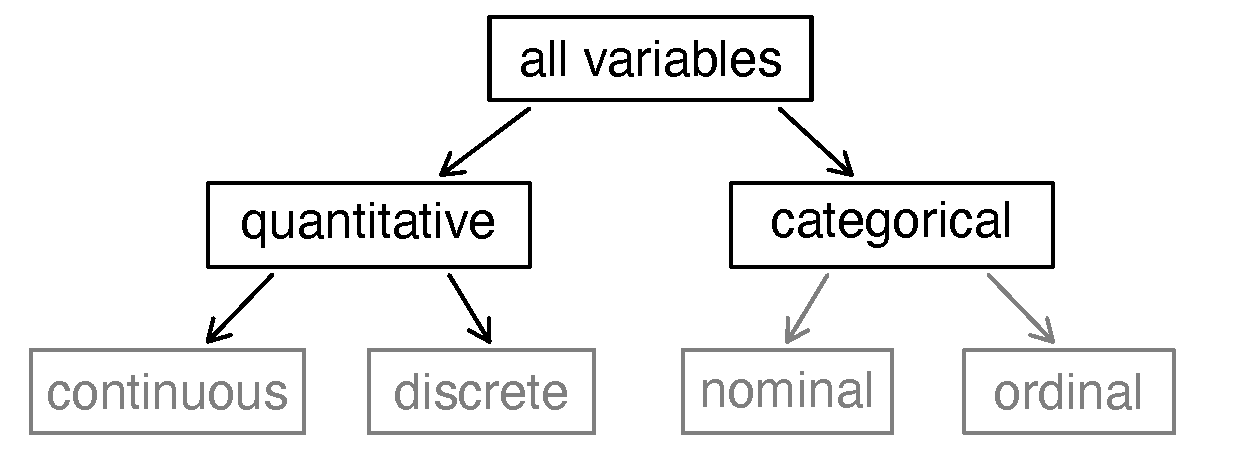
\includegraphics[width=0.5\linewidth]{images/variables} 

}

\caption{Types of variables.}\label{fig:types-of-variables}
\end{figure}

\begin{enumerate}
\def\labelenumi{\arabic{enumi}.}
\setcounter{enumi}{2}
\tightlist
\item
  One person from each group open the Google sheet linked in D2L and fill in the responses for the following questions for each group member. When creating a data set for use in R it is important to use single words or an underscore between words. Each outcome must be written the same way each time. Make sure to use all lowercase letters to create this data set to have consistency between responses. Do not give units of measure with the numerical values for the length of forearm. For \texttt{Residency} use in\_state or out\_state as the two outcomes.
\end{enumerate}

\begin{itemize}
\tightlist
\item
  Major: what is your declared major?
\item
  Residency: do you have in-state or out-of-state residency?
\item
  Forearm\_Length: what is the length of your forearm in inches from the end of your elbow to the end of your index finger?
\item
  Num\_Credits: how many credits are you taking this semester?
\end{itemize}

\begin{enumerate}
\def\labelenumi{\arabic{enumi}.}
\setcounter{enumi}{3}
\tightlist
\item
  For each column of data, fill in the following table to write out the variable we are collecting on each observational unit in this study and the type of each variable.
\end{enumerate}

\begin{center}
\begin{tabular}{|l|p{2.5in}|p{1.5in}|} \hline
Column & Variable & Type of Variable  \\ \hline
Major & & \\ 
& & \\ \hline
Residency & & \\ 
& & \\ \hline
Forearm Length & & \\ 
& & \\ \hline
Num Credits & & \\ 
& & \\ \hline
\end{tabular}
\end{center}

\begin{enumerate}
\def\labelenumi{\arabic{enumi}.}
\setcounter{enumi}{4}
\tightlist
\item
  Write down some issues found with the created class data set.
\end{enumerate}

\vspace{1in}

\hypertarget{take-home-messages}{%
\subsection{Take-home messages}\label{take-home-messages}}

\begin{enumerate}
\def\labelenumi{\arabic{enumi}.}
\item
  When creating a data set, each row will represent a single observational unit or case. Each column represents a variable collected. It is important to write each variable as a single word or use an underscore between words.
\item
  There are two types of variables: categorical (groups) and quantitative (numerical measures).
\item
  Make sure to be consistent with writing each outcome in the data set.
\end{enumerate}

\hypertarget{additional-notes}{%
\subsection{Additional notes}\label{additional-notes}}

Use this space to summarize your thoughts and take additional notes on today's activity and material covered, and to write down the names and contact information of your teammates.

\newpage

\hypertarget{week-1-lab---sampling-methods}{%
\section{Week 1 Lab - Sampling Methods}\label{week-1-lab---sampling-methods}}

\setstretch{1}

\hypertarget{learning-outcomes-1}{%
\subsection{Learning outcomes}\label{learning-outcomes-1}}

\begin{itemize}
\tightlist
\item
  Identify biased sampling methods.
\end{itemize}

\hypertarget{terminology-review-1}{%
\subsection{Terminology review}\label{terminology-review-1}}

Statistics is the study of how best to collect, analyze, and draw conclusions from data. Today in class you will be introduced to the following terms:

\begin{itemize}
\tightlist
\item
  Types of sampling bias

  \begin{itemize}
  \tightlist
  \item
    Selection bias
  \item
    Response bias
  \item
    Non-response bias
  \end{itemize}
\end{itemize}

For more on these concepts, read Chapter 1 and Section 2.1 in the textbook.

\hypertarget{general-information-on-labs}{%
\subsection{General information on labs}\label{general-information-on-labs}}

On Friday of each week you will complete a lab. Questions are selected from each lab to be turned in on Gradescope. The questions to be submitted on Gradescope are bolded in the lab. As you work through the lab have the Gradescope lab assignment open so that you can answer those questions as you go.

\hypertarget{types-of-bias}{%
\subsection*{Types of bias}\label{types-of-bias}}
\addcontentsline{toc}{subsection}{Types of bias}

In the next few weeks we will look at how to summarize data both numerically and graphically. For now we will focus on sampling methods and the type of sampling bias that may be present.

\begin{itemize}
\item
  Selection bias: a part of the target population is not included or underrepresented in the sample
\item
  Non-response or non-participation bias: part of the already selected sample does not respond or chooses not to participate
\item
  Response bias: survey participant gives an untruthful or misleading response
\end{itemize}

To help determine the type of bias present, it is helpful to think about the observational units, the sample, and the target population represented by the problem. The \textbf{target population} is the group of cases that makes up the population the researcher is interested in. If sampling bias is present, than the sample taken will not be representative of the actual target population. In these next questions, identify the target population, the sample selected, the variable collected and its type (categorical or quantitative), and the type of bias present.

\newpage

\begin{enumerate}
\def\labelenumi{\arabic{enumi}.}
\item
  \textbf{To determine if the proportion of out-of-state undergraduate students at Montana State University has increased in the last 10 years, a statistics instructor sent an email survey to 500 randomly selected current undergraduate students. One of the questions on the survey asked whether they had in-state or out-of-state residency. She only received 378 responses.}
  \vspace{0.25in}

  Sample size:
  \vspace{0.3in}

  Sample taken:
  \vspace{0.3in}

  Target population:
  \vspace{0.3in}

  Variable:
  \vspace{0.3in}

  Type of Variable: \hspace{1mm} categorical \hspace{0.2in} quantitative
  \vspace{1mm}

  Justify why there is non-response bias in this study.
  \vspace{0.5in}
\item
  A television station is interested in predicting whether or not a local referendum to legalize marijuana for adult use will pass. It asks its viewers to phone in and indicate whether they are in favor or opposed to the referendum. Of the 2241 viewers who phoned in, forty-five percent were opposed to legalizing marijuana.
  \vspace{0.1in}

  Sample size:
  \vspace{0.3in}

  Sample taken:
  \vspace{0.3in}

  Target population:
  \vspace{0.3in}

  Variable:
  \vspace{0.3in}

  Type of Variable: \hspace{1mm} categorical \hspace{0.2in} quantitative
  \vspace{1mm}

  Justify why there is selection bias in this study.
  \vspace{0.5in}
  \newpage
\item
  To gauge the interest in a new swimming pool, a local organization stood outside of the Bogart Pool in Bozeman, MT, during open hours. One of the questions they asked was, ``Since the Bogart Pool is in such bad repair, don't you agree that the city should fund a new pool?''
  \vspace{0.1in}

  Sample size:
  \vspace{0.3in}

  Sample taken:
  \vspace{0.3in}

  Target population:
  \vspace{0.3in}

  Variable:
  \vspace{0.3in}

  Type of Variable: \hspace{1mm} categorical \hspace{0.2in} quantitative
  \vspace{1mm}

  Justify why there is response bias in this study.
  \vspace{0.5in}

  Justify why there is selection bias in this study.
  \vspace{0.5in}
\item
  \textbf{The Bozeman school district was interested in surveying parents of students about their opinions on returning to in-person classes following the COVID-19 pandemic. They divided the school district into 10 divisions based on location and randomly surveyed 20 households within each division. Explain why selection bias would be present in this study design.}
  \vspace{1in}
\end{enumerate}

\newpage

\hypertarget{gas-prices}{%
\subsection*{Gas prices}\label{gas-prices}}
\addcontentsline{toc}{subsection}{Gas prices}

In this part of the lab we will explore two different websites to explore the cost of gas. Open both the Gas Buddy Website (www.gasbuddy.com) and a government website (\url{https://www.eia.gov/petroleum/}). Spend some time exploring each site.

\begin{enumerate}
\def\labelenumi{\arabic{enumi}.}
\setcounter{enumi}{4}
\tightlist
\item
  Choose a city listed on both sites. Write down three gas prices found on Gas Buddy for this city and the reported gas price from the government website for the same city.
\end{enumerate}

\vspace{0.5in}

\begin{enumerate}
\def\labelenumi{\arabic{enumi}.}
\setcounter{enumi}{5}
\tightlist
\item
  Compare the two websites.
\end{enumerate}

\begin{itemize}
\tightlist
\item
  Why are gas stations selected to appear in each data set?
\end{itemize}

\vspace{0.3in}

\begin{itemize}
\tightlist
\item
  Do we know if gas stations were left out for any given time period?
\end{itemize}

\vspace{0.3in}

\begin{itemize}
\tightlist
\item
  Can we make claims about what the mean price is for all gas stations in a region?
\end{itemize}

\vspace{0.3in}

\begin{enumerate}
\def\labelenumi{\arabic{enumi}.}
\setcounter{enumi}{6}
\tightlist
\item
  \textbf{Which of the following questions are best answered with the government data, and which with Gas Buddy?}
\end{enumerate}

\begin{itemize}
\tightlist
\item
  How do average gas prices compare across regions of the country?
\end{itemize}

\vspace{0.3in}

\begin{itemize}
\tightlist
\item
  Where should I go to buy gas right now?
\end{itemize}

\vspace{0.3in}

\begin{itemize}
\tightlist
\item
  What will prices be like in one week? One year?
\end{itemize}

\vspace{0.3in}

\hypertarget{take-home-messages-1}{%
\subsection{Take-home messages}\label{take-home-messages-1}}

\begin{enumerate}
\def\labelenumi{\arabic{enumi}.}
\tightlist
\item
  There are three types of bias to be aware of when designing a sampling method: selection bias, non-response bias, and response bias.
\end{enumerate}

\hypertarget{additional-notes-1}{%
\subsection{Additional notes}\label{additional-notes-1}}

Use this space to summarize your thoughts and take additional notes on today's activity and material covered, and to write down the names and contact information of your teammates.

\newpage

\hypertarget{study-design}{%
\chapter{Study Design}\label{study-design}}

\hypertarget{week-2-reading-guide-sampling-experimental-design-and-scope-of-inference}{%
\section{Week 2 Reading Guide: Sampling, Experimental Design, and Scope of Inference}\label{week-2-reading-guide-sampling-experimental-design-and-scope-of-inference}}

\hypertarget{sections-2.2-observational-studies-2.3-experiments-and-2.4-scope-of-inference}{%
\subsection*{Sections 2.2 (Observational studies), 2.3 (Experiments), and 2.4 (Scope of inference)}\label{sections-2.2-observational-studies-2.3-experiments-and-2.4-scope-of-inference}}
\addcontentsline{toc}{subsection}{Sections 2.2 (Observational studies), 2.3 (Experiments), and 2.4 (Scope of inference)}

\setstretch{1}

\textbf{Videos}

\begin{itemize}
\tightlist
\item
  2.2to2.4
\end{itemize}

\setstretch{1.25}

\hypertarget{reminders-from-section-1.2}{%
\subsubsection*{Reminders from Section 1.2}\label{reminders-from-section-1.2}}
\addcontentsline{toc}{subsubsection}{Reminders from Section 1.2}

\textbf{Explanatory variable}: The variable researchers think \emph{may be} affecting the other variable. What the researchers control/assign in an experiment. If comparing groups, the explanatory variable puts the observational units into groups.

\textbf{Response variable}: The variable researchers think \emph{may be} influenced by the other variable. This variable is always observed, never controlled or assigned.

\hypertarget{vocabulary-2}{%
\subsubsection*{Vocabulary}\label{vocabulary-2}}
\addcontentsline{toc}{subsubsection}{Vocabulary}

Observational study:
\rgs

\rgi Observational data:
\rgs

\rgi Prospective study:
\rgs

\rgi Retrospective study:
\rgs

Confounding variable:
\rgs

Experiment:
\rgs

\rgi Randomized experiment:
\rgs

\rgi Blocking:
\rgs

\rgi Treatment group:
\rgs

\rgi Control group:
\rgs

\rgi Blinding:
\rgs

\rgi Placebo:
\rgs

\rgi Placebo effect:
\rgs

Scope of inference:
\rgs

\rgi Generalizability:
\rgs

\rgi Causation:
\rgs

\hypertarget{notes-2}{%
\subsubsection*{Notes}\label{notes-2}}
\addcontentsline{toc}{subsubsection}{Notes}

What are the four principles of a well-designed randomized experiment?\\
\rgs
\rgs
\rgs

Fill in the appropriate scope of inference for each study design.

\begin{center}
\begin{tabular}{|p{2in}|p{2in}|p{2in}|}
\hline
 & \multicolumn{2}{|c|}{\textbf{Study Type}} \\ \hline
 \textbf{Selection of Cases} & Randomized experiment & Observational study \\ \hline
 Random sample && \\ 
 (and no other sampling bias) & & \\ 
  & & \\
   & & \\ \hline
   Non-random sample && \\ 
   (or other sampling bias) & & \\ 
  & & \\
   & & \\ \hline
\end{tabular}
\end{center}

\rgs

True or False: Observational studies can show an association between two variables, but cannot determine a causal relationship.

True or False: In order for an experiment to be valid, a placebo must be used.

True or False: If random sampling of the target population is used, and no other types of bias are suspected, results from the sample can be generalized to the entire target population.

True or False: If random sampling of the target population is used, and no other types of bias are suspected, results from the sample can be inferred as a causal relationship between the explanatory and response variables.

\newpage

\hypertarget{activity-2a-american-indian-address}{%
\section{Activity 2A: American Indian Address}\label{activity-2a-american-indian-address}}

\setstretch{1}

\hypertarget{learning-outcomes-2}{%
\subsection{Learning outcomes}\label{learning-outcomes-2}}

\begin{itemize}
\item
  Explain why a sampling method is unbiased or biased.
\item
  Identify biased sampling methods.
\item
  Explain the purpose of random selection and its effect on scope of inference.
\end{itemize}

\hypertarget{terminology-review-2}{%
\subsection{Terminology review}\label{terminology-review-2}}

In today's activity, we will examine unbiased and biased methods of sampling. Some terms covered in this activity are:

\begin{itemize}
\item
  Random sample
\item
  Unbiased vs biased methods of selection
\item
  Generalization
\end{itemize}

To review these concepts, see Section 2.1 in the textbook.

\hypertarget{american-indian-address}{%
\subsection{American Indian Address}\label{american-indian-address}}

For this activity, you will read a speech given by Jim Becenti, a member of the Navajo American Indian tribe, who spoke about the employment problems his people faced at an Office of Indian Affairs meeting in Phoenix, Arizona, on January 30, 1947 (Moquin and Van Doren 1973). His speech is below:

\textbf{It is hard for us to go outside the reservation where we meet strangers. I have been off the reservation ever since I was sixteen. Today I am sorry I quit the Santa Fe {[}Railroad{]}. I worked for them in 1912-13. You are enjoying life, liberty, and happiness on the soil the American Indian had, so it is your responsibility to give us a hand, brother. Take us out of distress. I have never been to vocational school. I have very little education. I look at the white man who is a skilled laborer. When I was a young man I worked for a man in Gallup as a carpenter's helper. He treated me as his own brother. I used his tools. Then he took his tools and gave me a list of tools I should buy and I started carpentering just from what I had seen. We have no alphabetical language.}

\textbf{We see things with our eyes and can always remember it. I urge that we help my people to progress in skilled labor as well as common labor. The hope of my people is to change our ways and means in certain directions, so they can help you someday as taxpayers. If not, as you are going now, you will be burdened the rest of your life. The hope of my people is that you will continue to help so that we will be all over the United States and have a hand with you, and give us a brotherly hand so we will be happy as you are. Our reservation is awful small. We did not know the capacity of the range until the white man come and say ``you raise too much sheep, got to go somewhere else,'' resulting in reduction to a skeleton where the Indians can't make a living on it. For eighty years we have been confused by the general public, and what is the condition of the Navajo today? Starvation! We are starving for education. Education is the main thing and the only thing that is going to make us able to compete with you great men here talking to us.}

\hypertarget{by-eye-selection}{%
\subsubsection*{By eye selection}\label{by-eye-selection}}
\addcontentsline{toc}{subsubsection}{By eye selection}

\begin{enumerate}
\def\labelenumi{\arabic{enumi}.}
\tightlist
\item
  Circle ten words in Jim Becenti's speech which are a representative sample of the length of words in the entire text. Describe your method for selecting this sample.
\end{enumerate}

\vspace{0.3in}

\begin{enumerate}
\def\labelenumi{\arabic{enumi}.}
\setcounter{enumi}{1}
\tightlist
\item
  Fill in the table below with the length of each word (number of letters/digits in the word) selected in question 1:
  \vspace{1mm}
\end{enumerate}

\begin{center}
\begin{tabular}{|l|p{1in}|} \hline
Observation & Length  \\ \hline
1 &  \\ 
&  \\ \hline
2 &  \\ 
&  \\ \hline
3 & \\ 
&  \\ \hline
4 & \\ 
& \\ \hline
5 & \\ 
& \\ \hline
6 & \\ 
& \\ \hline
7 & \\
& \\ \hline
8 & \\ 
& \\ \hline
9 & \\ 
& \\ \hline
10 & \\ 
& \\ \hline
\end{tabular}
\end{center}

\begin{enumerate}
\def\labelenumi{\arabic{enumi}.}
\setcounter{enumi}{2}
\item
  Calculate the mean (average) word length in your selected sample. Is this value a parameter or a statistic?\\
  \vspace{0.3in}
\item
  Report your mean word length to your instructor. Your instructor will guide the class in creating a visualization of the distribution of results generated by your class. Draw a picture of the plot here. Include a descriptive \(x\)-axis label.
  \vspace{1.5in}
\item
  Based on the plot of sample mean word lengths in question 4, what is your best guess for the average word length of the population of all 359 words in the speech?
  \vspace{0.3in}
\item
  The true mean word length of the population of all 359 words in the speech is 3.95 letters. Is this value a parameter or a statistic?\\
  \vspace{0.2in}

  Where does the value of 3.95 fall in the plot created in question 4? Near the center of the distribution? In the tails of the distribution?
  \vspace{0.3in}
\item
  If the class samples were truly representative of the population of words, what proportion of sample means would you expect to be below 3.95?
  \vspace{0.5in}
\item
  Using the graph created in question 4, estimate the proportion of students' computed sample means that were lower than the true mean of 3.95 letters?
  \vspace{0.5in}
\item
  Based on your answers to questions 7 and 8, would you say the sampling method used by the class is biased or unbiased? Justify your answer.\\
  \vspace{0.5in}
\item
  If the sampling method is biased, what type of sampling bias (selection, response, non-response) is present? What is the direction of the bias, i.e., does the method tend to overestimate or underestimate the population mean word length?
  \vspace{0.5in}
\item
  Should we use results from our by eye samples to make a statement about the word length in the population of words in Becenti's address? Why or why not?
  \vspace{1in}
\end{enumerate}

\hypertarget{take-home-messages-2}{%
\subsection{Take-home messages}\label{take-home-messages-2}}

\begin{enumerate}
\def\labelenumi{\arabic{enumi}.}
\item
  When we use a biased method of sample selection, the method will tend to overestimate or underestimate the parameter.
\item
  To see if a method is biased, we compare the distribution of the estimates to the true value. We want our estimate to be on target or unbiased. When using unbiased methods of selection, the mean of the distribution matches or is very similar to our true parameter.
\item
  If the sampling method is biased, inferences made about the population based on a sample estimate will not be valid.
\end{enumerate}

\hypertarget{additional-notes-2}{%
\subsection{Additional notes}\label{additional-notes-2}}

Use this space to summarize your thoughts and take additional notes on today's activity and material covered.

\newpage

\hypertarget{activity-2b-american-indian-address-continued}{%
\section{Activity 2B: American Indian Address (continued)}\label{activity-2b-american-indian-address-continued}}

\setstretch{1}

\hypertarget{learning-outcomes-3}{%
\subsection{Learning outcomes}\label{learning-outcomes-3}}

\begin{itemize}
\item
  Explain the purpose of random selection and its effect on scope of inference.
\item
  Select a simple random sample from a finite population using a random number generator.
\item
  Explain why a sampling method is unbiased or biased.
\item
  Explain the effect of sample size on sampling variability.
\end{itemize}

\hypertarget{terminology-review-3}{%
\subsection{Terminology review}\label{terminology-review-3}}

In today's activity, we will examine unbiased and biased methods of sampling. Some terms covered in this activity are:

\begin{itemize}
\item
  Random sample
\item
  Unbiased vs biased methods of selection
\item
  Generalization
\end{itemize}

To review these concepts, see Section 2.1 in the textbook.

\hypertarget{random-selection}{%
\subsubsection*{Random selection}\label{random-selection}}
\addcontentsline{toc}{subsubsection}{Random selection}

Today we will return to the American Indian Address introduced in Activity 2A. Suppose instead of attempting to select a representative sample by eye (which did not work), each student used a random number generator to select a simple random sample of 10 words. A \textbf{simple random sample} relies on a random mechanism to choose a sample, without replacement, from the population, such that every sample of size 10 is equally likely to be chosen.

To use a random number generator to select a simple random sample, you first need a numbered list of all the words in the population, called a \textbf{sampling frame}. You can then generate 10 random numbers from the numbers 1 to 359 (the number of words in the population), and the chosen random numbers correspond to the chosen words in your sample.

\begin{enumerate}
\def\labelenumi{\arabic{enumi}.}
\tightlist
\item
  Use the random number generator at \url{https://istats.shinyapps.io/RandomNumbers/} to select a simple random sample from the population of all 359 words in the speech.
\end{enumerate}

\begin{itemize}
\item
  Set ``Choose Minimum'' to 1 and ``Choose Maximum'' to 359 to represent the 359 words in the population (the sampling frame).
\item
  Set ``How many numbers do you want to generate?'' to 10 and ensure the ``No'' option is selected under ``Sample with Replacement?''
\item
  Click ``Generate''.
\end{itemize}

\newpage

Fill in the table below with the random numbers selected and use the \textbf{Becenti.csv data file} found on D2L to determine each number's corresponding word and word length (number of letters/digits in the word):

\begin{center}
\begin{tabular}{|l|l|p{1in}|} \hline
Observation & Number & Length  \\ \hline
1 & & \\ 
& & \\ \hline
2 & & \\ 
& & \\ \hline
3 & & \\ 
& & \\ \hline
4 & & \\ 
& & \\ \hline
5 & & \\ 
& & \\ \hline
6 & & \\ 
& & \\ \hline
7 & & \\
& & \\ \hline
8 & & \\ 
& & \\ \hline
9 & & \\ 
& & \\ \hline
10 & & \\ 
& & \\ \hline
\end{tabular}
\end{center}

\begin{enumerate}
\def\labelenumi{\arabic{enumi}.}
\setcounter{enumi}{1}
\item
  Calculate the mean word length in your selected sample in question 1. Is this value a parameter or a statistic?
  \vspace{0.3in}
\item
  Report your mean word length to your instructor. Your instructor will guide the class in creating a visualization of the distribution of results generated by your class. Draw a picture of the plot here. Include a descriptive \(x\)-axis label.
  \vspace{1.7in}
\item
  Where does the value 3.95, the true mean word length, fall in the distribution created in question 3? Near the center of the distribution? In the tails of the distribution?
  \vspace{0.3in}
\end{enumerate}

\newpage

One set of randomly generated sample mean word lengths from a single class may not be large enough to visualize the distribution results. Let's have a computer generate 1,000 sample mean word lengths for us.

\begin{itemize}
\item
  Navigate to the ``One Variable with Sampling'' Rossman/Chance web applet: \url{http://www.rossmanchance.com/applets/2021/sampling/OneSample.html?population=gettysburg}.
\item
  Click ``Clear'' below the text box containing data from the Gettysburg address to delete that data set.
\item
  Download the Becenti.csv file from D2L and open the spreadsheet on your computer.
\item
  Copy and paste the population of word lengths (column C) into the applet from the data set provided making sure to include the header. Click ``Use Data''. Verify that the mean for the data set is 3.953 with a sample size of 359. If these are not the values you got, check with your instructor for help with copying in the data set correctly.
\item
  Click the check-box for ``Show Sampling Options''
\item
  Select 1000 for ``Number of samples'' and select 10 for the ``Sample size''.
\item
  Click ``Draw Samples''.
\end{itemize}

\begin{enumerate}
\def\labelenumi{\arabic{enumi}.}
\setcounter{enumi}{4}
\item
  The plot labeled ``Statistics'' displays the 1,000 randomly generated sample mean word lengths. Sketch this plot below. Include a descriptive \(x\)-axis label and be sure to write down the provided mean and SD (standard deviation) of the distribution.
  \vspace{2in}
\item
  What is the center value of the distribution created in question 5?
  \vspace{0.3in}
\item
  Explain why the sampling method of using a random number generator to generate a sample is a ``better'' method than choosing 10 words ``by eye''.
  \vspace{0.8in}
\item
  Is random selection an unbiased method of selection? Explain your answer. Be sure to reference your plot from question 5.
  \vspace{0.5in}
\end{enumerate}

\hypertarget{effect-of-sample-size}{%
\subsection*{Effect of sample size}\label{effect-of-sample-size}}
\addcontentsline{toc}{subsection}{Effect of sample size}

We will now consider the impact of sample size.

\begin{enumerate}
\def\labelenumi{\arabic{enumi}.}
\setcounter{enumi}{8}
\item
  First, consider if each student had selected 20 words, instead of 10, by eye. Do you think this would make the plot from question 4 in Activity 2A centered on 3.95 (the true mean word length)? Explain your answer.
  \vspace{0.4in}
\item
  Now we will select 20 words instead of 10 words at random.
\end{enumerate}

\begin{itemize}
\item
  In the ``One Variable with Sampling'' Rossman/Chance web applet(\url{http://www.rossmanchance.com/applets/2021/sampling/OneSample.html?population=gettysburg}.), change the Sample size to 20.
\item
  Click ``Draw Samples''.
\end{itemize}

The plot labeled ``Statistics'' displays the 1,000 randomly generated sample mean word lengths. Sketch this plot below. Include a descriptive \(x\)-axis label and be sure to write down the provided mean and SD (standard deviation) of the distribution.
\vspace{1.6in}

\begin{enumerate}
\def\labelenumi{\arabic{enumi}.}
\setcounter{enumi}{10}
\tightlist
\item
  Compare the distribution created in question 10 to the one created in question 5.
\end{enumerate}

\rgi Which features are similar?\\
\vspace{0.3in}

\rgi Which features differ?

\vspace{0.3in}

\newpage

\begin{enumerate}
\def\labelenumi{\arabic{enumi}.}
\setcounter{enumi}{11}
\item
  Compare the spreads of the plots in question 10 and in question 5. You should see that in one plot all sample means are closer to the population mean than in the other. Which plot shows this?
  \vspace{0.4in}
\item
  Using the evidence from your simulations, answer the following questions:
\end{enumerate}

\rgi Does changing the sample size impact whether the sample estimates are unbiased? Explain your answer.
\vspace{0.5in}

\rgi Does changing the sample size impact the variability (spread) of sample estimates? Explain your answer
\vspace{0.5in}

\begin{enumerate}
\def\labelenumi{\arabic{enumi}.}
\setcounter{enumi}{13}
\tightlist
\item
  What is the purpose of random selection of a sample from the population?
\end{enumerate}

\vspace{0.8in}

\hypertarget{take-home-messages-3}{%
\subsection{Take-home messages}\label{take-home-messages-3}}

\begin{enumerate}
\def\labelenumi{\arabic{enumi}.}
\item
  Random selection is an unbiased method of selection.
\item
  To determine if a sampling method is biased or unbiased, we compare the distribution of the estimates to the true value. We want our estimate to be on target or unbiased. When using unbiased methods of selection, the mean of the distribution matches or is very similar to our true parameter.
\item
  Random selection eliminates selection bias. However, random selection will not eliminate response or non-response bias.
\item
  The larger the sample size, the more similar (less variable) the statistics will be from different samples.
\item
  Sample size has no impact on whether a \emph{sampling method} is biased or not. Taking a larger sample using a biased method will still result in a sample that is not representative of the population.
\end{enumerate}

\hypertarget{additional-notes-3}{%
\subsection{Additional notes}\label{additional-notes-3}}

Use this space to summarize your thoughts and take additional notes on today's activity and material covered.

\newpage

\hypertarget{week-2-lab-study-design}{%
\section{Week 2 Lab: Study Design}\label{week-2-lab-study-design}}

\setstretch{1}

\hypertarget{learning-outcomes-4}{%
\subsection{Learning outcomes}\label{learning-outcomes-4}}

\begin{itemize}
\item
  Explain the purpose of random assignment and its effect on scope of inference.
\item
  Identify whether a study design is observational or an experiment.
\item
  Identify confounding variables in observational studies and explain why they are confounding.
\end{itemize}

\hypertarget{terminology-review-4}{%
\subsection{Terminology review}\label{terminology-review-4}}

In this activity, we will examine different study designs, confounding variables, and how to determine the scope of inference for a study. Some terms covered in this activity are:

\begin{itemize}
\item
  Scope of inference
\item
  Explanatory variable
\item
  Response variable
\item
  Confounding variable
\item
  Experiment
\item
  Observational study
\end{itemize}

To review these concepts, see Sections 2.2 through 2.5 in the textbook.

\hypertarget{general-information-labs}{%
\subsection{General information labs}\label{general-information-labs}}

Remember that each Friday you will complete a lab. Questions are selected from each lab to be turned in on Gradescope. The questions to be submitted on Gradescope are bolded in the lab. As you work through the lab have the Gradescope lab assignment open so that you can answer those questions as you go.

\hypertarget{atrial-fibrillation}{%
\subsection*{Atrial fibrillation}\label{atrial-fibrillation}}
\addcontentsline{toc}{subsection}{Atrial fibrillation}

Atrial fibrillation is an irregular and often elevated heart rate. In some people, atrial fibrillation will come and go on its own, but others will experience this condition on a permanent basis. When atrial fibrillation is constant, medications are required to stabilize the patient's heart rate and to help prevent blood clots from forming. Pharmaceutical scientists at a large pharmaceutical company believe they have developed a new medication that effectively stabilizes heart rates in people with permanent atrial fibrillation. They set out to conduct a trial study to investigate the new drug. The scientists will need to compare the proportion of patients whose heart rate is stabilized between two groups of subjects, one of whom is given a placebo and the other given the new medication.

\begin{enumerate}
\def\labelenumi{\arabic{enumi}.}
\item
  Identify the explanatory and response variable in this trial study.

  Explanatory variable:
  \vspace{0.5in}

  Response variable:
  \vspace{0.5in}
\end{enumerate}

\newpage

Suppose 24 subjects with permanent atrial fibrillation have volunteered to participate in this study. There are 16 subjects that self-identified as male and 8 subjects that self-identified as female.

\begin{enumerate}
\def\labelenumi{\arabic{enumi}.}
\setcounter{enumi}{1}
\item
  One way to separate into two groups would be give all the males the placebo and all the females the new drug. Explain why this is not a reasonable strategy.
  \vspace{1in}
\item
  Could the scientists fix the problem with the strategy presented in question 2 by creating equal sized groups by putting 4 males and 8 females into the drug group and the remaining 12 males in the placebo group? Explain your answer.
  \vspace{0.5in}
\item
  A third strategy would be to \textbf{block} on sex. In this type of study, the scientists would assign 4 females and 8 males to each group. Using this strategy, what \textbf{proportion} of males out of the 12 individuals would be in each group?
  \vspace{0.3in}
\item
  \textbf{Assume the scientists used the strategy in question 4, but they put the four tallest females and eight tallest males into the placebo group and the remaining subjects into the control group. They found that the proportion of patients whose heart rate stabilized is higher in the drug group than the placebo group.}\\
  \vspace{0.1in}

  Could that difference be due to the sex of the subjects? Explain your answer.
  \vspace{0.5in}

  Could it be due to other variables? Explain your answer.
  \vspace{0.5in}
\end{enumerate}

While the strategy presented in question 5 controlled for the sex of the subject, there are more potential \textbf{confounding variables} in the study. A confounding variable is a variable that is \emph{both}

\begin{enumerate}
\def\labelenumi{\arabic{enumi}.}
\tightlist
\item
  associated with the explanatory variable, \emph{and}
\item
  associated with the response variable.
\end{enumerate}

When both these conditions are met, if we observe an association between the explanatory variable and the response variable in the data, we cannot be sure if this association is due to the explanatory variable or the confounding variable---the explanatory and confounding variables are ``confounded.''

\textbf{Random assignment} means that subjects in a study have an equally likely chance of receiving any of the available treatments.

\newpage

\begin{enumerate}
\def\labelenumi{\arabic{enumi}.}
\setcounter{enumi}{5}
\tightlist
\item
  You will now investigate how randomly assigning subjects impacts a study's scope of inference.
\end{enumerate}

\begin{itemize}
\item
  Navigate to the ``Randomizing Subjects'' applet under the ``Other Applets'' heading at: \url{http://www.rossmanchance.com/ISIapplets.html}. This applet lists the sex and height of each of the 24 subjects. Click ``Show Graphs'' to see a bar chart showing the sex of each subject. Currently, the applet is showing the strategy outlined in question 7.
\item
  Click ``Randomize''.
\end{itemize}

~~~In this random assignment, what proportion of males are in group 1 (the placebo group)?

\vspace{0.1in}

~~~What proportion of males are in group 2 (the drug group)?

\vspace{0.1in}

~~~What is the difference in proportion of males between the two groups (placebo - drug)?

\vspace{0.1in}

\begin{enumerate}
\def\labelenumi{\arabic{enumi}.}
\setcounter{enumi}{6}
\item
  Notice the difference in the two proportions is shown as a dot in the plot at the bottom of the web page. Un-check the box for Animate above ``Randomize'' and click ``Randomize'' again. Did you get the same difference in proportion of males between the placebo and drug groups?
  \vspace{0.25in}
\item
  Change ``Replications'' to 998 (for 1000 total). Click ``Randomize'' again. Sketch the plot of the distribution of difference in proportions from each of the 1000 random assignments here. Be sure to include a descriptive \(x\)-axis label.
  \vspace{1.25in}
\item
  \textbf{Does random assignment \emph{always} balance the placebo and drug groups based on the sex of the participants? Does random assignment \emph{tend} to make the placebo and drug groups \emph{roughly} the same with respect to the distribution of sex? Use your plot from question 8 to justify your answers.}
  \vspace{0.5in}
\item
  Change the drop-down menu below Group 2 from ``sex'' to ``height''. The applet now calculates the average height in the placebo and drug groups for each of the 1000 random assignments. The dot plot displays the distribution of the difference in mean heights (placebo - drug) for each random assignment. Based on this dot plot, is height distributed equally, on average, between the two groups? Explain how you know.
  \vspace{0.5in}
\end{enumerate}

\newpage

The diagram below summarizes these ideas about confounding variables and random assignment. When a confounding variable is present (such as sex or height), and an association is found in a study, it is impossible to discern what caused the change in the response variable. Is the change the result of the explanatory variable or the confounding variable? However, if all confounding variables are \emph{balanced} across the treatment groups, then only the explanatory variable differs between the groups and thus \emph{must have caused} the change seen in the response variable.

\begin{center}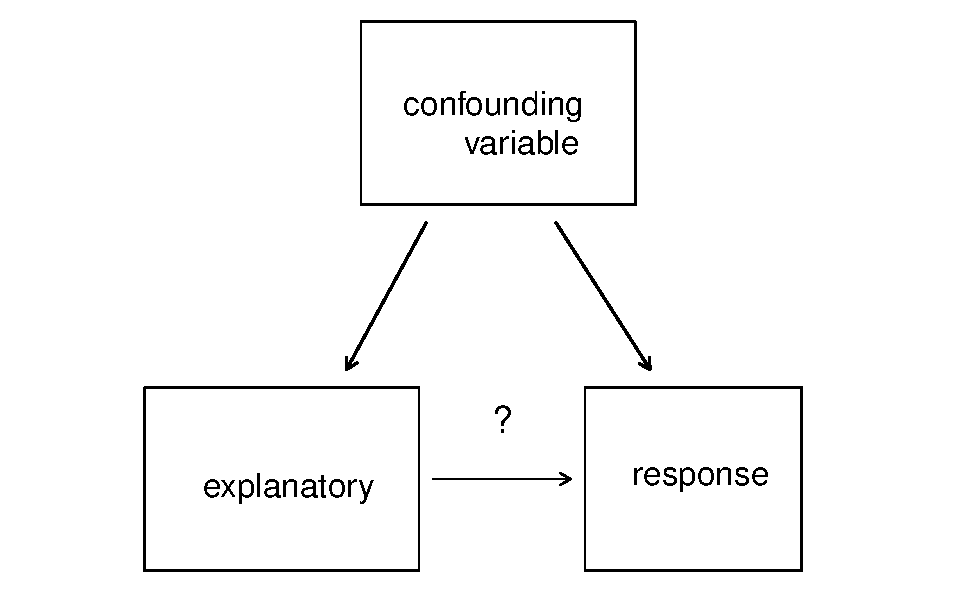
\includegraphics[width=0.4\linewidth]{02-L02-random-assignment_files/figure-latex/unnamed-chunk-1-1} \end{center}

\begin{enumerate}
\def\labelenumi{\arabic{enumi}.}
\setcounter{enumi}{10}
\item
  \textbf{What is the purpose of random assignment of the subjects in a study to the explanatory variable groups?}
  \vspace{0.8in}
\item
  Suppose in this study on atrial fibrillation, the scientists did randomly assign groups and found that the drug group has a higher proportion of subjects whose heart rates stabilized than the placebo group. Can the scientists conclude the new drug \emph{caused} the increased chance of stabilization? Explain your answer.
  \vspace{0.5in}
\item
  Is the sample of subjects a simple random sample or a convenience sample?
\end{enumerate}

\vspace{0.2in}

\begin{enumerate}
\def\labelenumi{\arabic{enumi}.}
\setcounter{enumi}{13}
\tightlist
\item
  \textbf{Both the sampling method (which we covered last week) and the study design will help to determine the \emph{scope of inference} for a study: To \emph{whom} can we generalize, and can we conclude \emph{causation or only association}? Use the table below to determine the scope of inference of this trial study described in question 12.}
  \vspace{0.3in}
\end{enumerate}

\begin{center}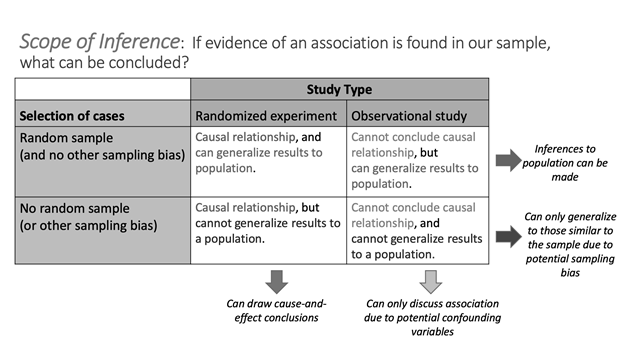
\includegraphics[width=0.75\linewidth]{images/ScopeOfInferenceGreyscale} \end{center}

\hypertarget{study-design-1}{%
\subsection*{Study design}\label{study-design-1}}
\addcontentsline{toc}{subsection}{Study design}

The two main study designs we will cover are \textbf{observational studies} and \textbf{experiments}. In observational studies, researchers have no influence over which subjects are in each group being compared (though they can control other variables in the study). An experiment is defined by assignment of the treatment groups of the \emph{explanatory variable}, typically via random assignment. In today's activity we will discover the purpose behind random assignment.

For the next exercises identify the study design (observational study or experiment), the sampling method, and the scope of inference.

\begin{enumerate}
\def\labelenumi{\arabic{enumi}.}
\setcounter{enumi}{14}
\item
  The pharmaceutical company Moderna Therapeutics, working in conjunction with the National Institutes of Health, conducted Phase 3 clinical trials of a vaccine for COVID-19 last fall. US clinical research sites enrolled 30,000 volunteers without COVID-19 to participate. Participants were randomly assigned to receive either the candidate vaccine or a saline placebo. They were then followed to assess whether or not they developed COVID-19. The trial was double-blind, so neither the investigators nor the participants knew who was assigned to which group.
  \vspace{0.1in}

  Study design:
  \vspace{0.25in}

  Sampling method:
  \vspace{0.25in}

  Scope of inference:
  \vspace{0.25in}
\item
  \textbf{In another study, a local health department randomly selected 1000 US adults without COVID-19 to participate in a health survey. Each participant was assessed at the beginning of the study and then followed for one year. They were interested to see which participants elected to receive a vaccination for COVID-19 and whether any participants developed COVID-19.}
  \vspace{0.1in}

  Study design:
  \vspace{0.25in}

  Sampling method:
  \vspace{0.25in}

  Scope of inference:
  \vspace{0.25in}
\end{enumerate}

\hypertarget{take-home-messages-4}{%
\subsection{Take-home messages}\label{take-home-messages-4}}

\begin{enumerate}
\def\labelenumi{\arabic{enumi}.}
\item
  The study design (observational study vs, experiment) determines if we can draw causal inferences or not. If an association is detected, a randomized experiment allows us to conclude that there is a causal (cause-and-effect) relationship between the explanatory and response variable. Observational studies have potential confounding variables within the study that prevent us from inferring a causal relationship between the variables studied.
\item
  Confounding variables are variables not included in the study that are related to both the explanatory and the response variables. When there are potential confounding variables in the study we cannot draw causal inferences.
\item
  Random assignment balances confounding variables across treatment groups. This eliminates any possible confounding variables by breaking the connections between the explanatory variable and the potential confounding variables.
\item
  Observational studies will always carry the possibility of confounding variables. Randomized experiments, which use random assignment, will have no confounding variables.
\end{enumerate}

\newpage

\hypertarget{additional-notes-4}{%
\subsection{Additional notes}\label{additional-notes-4}}

Use this space to summarize your thoughts and take additional notes on today's activity and material covered.

\newpage

\hypertarget{exploring-categorical-and-quantitative-data}{%
\chapter{Exploring Categorical and Quantitative Data}\label{exploring-categorical-and-quantitative-data}}

\hypertarget{week-3-reading-guide-introduction-to-r-categorical-variables-and-a-single-quantitative-variable}{%
\section{Week 3 Reading Guide: Introduction to R, Categorical Variables, and a Single Quantitative Variable}\label{week-3-reading-guide-introduction-to-r-categorical-variables-and-a-single-quantitative-variable}}

\hypertarget{chapter-3-applications-data}{%
\subsection*{Chapter 3 (Applications: Data)}\label{chapter-3-applications-data}}
\addcontentsline{toc}{subsection}{Chapter 3 (Applications: Data)}

\textbf{Videos}

\begin{itemize}
\tightlist
\item
  Starting\_with\_R
\end{itemize}

\setstretch{1.25}

\hypertarget{notes-3}{%
\subsubsection*{Notes}\label{notes-3}}
\addcontentsline{toc}{subsubsection}{Notes}

R is case sensitive, meaning it reads \texttt{data} differently from \texttt{Data}. If you get an error message, check that your capitalization is correct.

R does not like spaces or special characters. This means the column and row headers in the data set should not have spaces, periods, commas, etc. Instead of titling the variable \texttt{column\ header}, use \texttt{column\_header} or \texttt{ColumnHeader}.

\textbf{Tidy data}: Data frames should have

\rgi 1 row per \_\_\_\_\_\_\_\_\_\_\_\_\_\_\_\_,

\rgi 1 column per \_\_\_\_\_\_\_\_\_\_\_\_.

We highly recommend completing the R/RStudio tutorials in section 3 to help understand R better.

We will not expect you to be able to write full code independently for this course. For Stat 216, you will need to understand types (categorical or quantitative) and roles (explanatory or response) of variables, as well as the structure of data, in order to fill in a few blanks in provided code to graph or analyze data.

\hypertarget{functions}{%
\subsubsection*{Functions}\label{functions}}
\addcontentsline{toc}{subsubsection}{Functions}

State what these introductory functions do in R:

\texttt{glimpse(data\_set\_name)}

\texttt{head(data\_set\_name)}

\texttt{data\_set\_name\$variable\_name}

\texttt{\textless{}-}

\texttt{\%\textgreater{}\%}

\hypertarget{chapter-4-exploring-categorical-data}{%
\subsection*{Chapter 4 (Exploring categorical data)}\label{chapter-4-exploring-categorical-data}}
\addcontentsline{toc}{subsection}{Chapter 4 (Exploring categorical data)}

\setstretch{1}

\textbf{Videos}

\begin{itemize}
\tightlist
\item
  4.1
\item
  4.2
\item
  4.4
\end{itemize}

\setstretch{1.25}

\hypertarget{vocabulary-3}{%
\subsubsection*{Vocabulary}\label{vocabulary-3}}
\addcontentsline{toc}{subsubsection}{Vocabulary}

Frequency table:
\rgs

Relative frequency table:
\rgs

Contingency or two-way table:
\rgs

Association (between two variables):
\rgs

Unconditional proportion:
\rgs

Conditional proportion:
\rgs

\rgi Row proportions:
\rgs

\rgi Column proportions:
\rgs

Statistic:
\rgs

\rgi Sample proportion:
\rgs

\rgi \rgi Notation:
\rgs

Parameter:
\rgs

\rgi Population proportion:
\rgs

\rgi \rgi Notation:
\rgs

Bar plot:
\rgs

Segmented bar plot:
\rgs

Mosaic plot:
\rgs

Simpson's Paradox:
\rgs

\hypertarget{notes-4}{%
\subsubsection*{Notes}\label{notes-4}}
\addcontentsline{toc}{subsubsection}{Notes}

In a contingency table, which variable (explanatory or response) generally will make the columns of the table? Which variable will make the rows of the table?
\rgs

In a segmented bar plot, the bars represent the levels of which variable? The segments represent the levels of which variable?
\rgs

What type of plot(s) are appropriate to display a single categorical variable?
\rgs

What type of plot(s) are appropriate to display two categorical variables?
\rgs

What is the difference between a standardized segmented bar plot and a mosaic plot?
\rgs

True or false: Pie charts are generally highly recommended ways to graphically display categorical data.

True or false: Two categorical variables are associated if the conditional proportions of a particular outcome (typically of the response variable) differ across levels of the other variable (typically the explanatory variable).

True or false: When a segmented bar plot has segments that sum to 1 (or 100\%), the segment heights correspond to the proportions conditioned on the \textbf{segment}.

\hypertarget{review-of-simpsons-paradox}{%
\subsubsection*{Review of Simpson's Paradox}\label{review-of-simpsons-paradox}}
\addcontentsline{toc}{subsubsection}{Review of Simpson's Paradox}

Based on the segmented bar plot in Figure 4.6, which race of defendant was more likely to have the death penalty invoked?
\rgs

Based on the segmented bar plot in Figure 4.7 and Table 4.9, which race of defendant was more likely to have the death penalty invoked when the victim was Caucasian?
\rgs

Based on the segmented bar plot in Figure 4.7 and Table 4.9, which race of defendant was more likely to have the death penalty invoked when the victim was African American?
\rgs

The direction of the relationship between the \_\_\_\_\_\_\_\_\_\_\_\_\_\_
and \_\_\_\_\_\_\_\_\_\_\_\_\_\_ variables is \textbf{reversed} when accounting for
a \_\_\_\_\_\_\_\_\_\_\_\_\_\_ variable.
\rgs

\hypertarget{chapter-5-exploring-quantitative-data}{%
\subsection*{Chapter 5 (Exploring quantitative data)}\label{chapter-5-exploring-quantitative-data}}
\addcontentsline{toc}{subsection}{Chapter 5 (Exploring quantitative data)}

\textbf{Videos}

\begin{itemize}
\tightlist
\item
  5.2to5.4
\item
  5.5to5.6
\item
  5.7
\end{itemize}

\hypertarget{type-of-plots}{%
\subsubsection*{Type of Plots}\label{type-of-plots}}
\addcontentsline{toc}{subsubsection}{Type of Plots}

Scatterplot:
\rgs

Dot plot:
\rgs

Histogram:
\rgs

Density plot:
\rgs

Box plot:
\rgs

\hypertarget{vocabulary-4}{%
\subsubsection*{Vocabulary}\label{vocabulary-4}}
\addcontentsline{toc}{subsubsection}{Vocabulary}

Four characteristics of a scatterplot:

\rgi Form:
\rgs

\rgi Strength:
\rgs

\rgi Direction:
\rgs

\rgi Unusual observations or outliers:
\rgs

Distribution (of a variable):
\rgs

\rgi Four characteristics of the distribution of one quantitative variable:

\rgi Center:
\rgs

\rgi Variability:
\rgs

\rgi Shape:
\rgs

\rgi Outliers:
\rgs

Point estimate:
\rgs

Histogram:
\rgs

Data density:
\rgs

Tail:
\rgs

Skew:
\rgs

Symmetric:
\rgs

Modality:
\rgs

Density plot:
\rgs 

Deviation:
\rgs

Variance:
\rgs

Standard deviation:
\rgs

Boxplot:
\rgs

Five number summary:
\rgs

Median:
\rgs

\(X^{th}\) percentile:
\rgs

Interquartile range (IQR):
\rgs

Robust statistics:
\rgs

\hypertarget{notes-5}{%
\subsubsection*{Notes}\label{notes-5}}
\addcontentsline{toc}{subsubsection}{Notes}

What type of plot(s) are appropriate for displaying one quantitative variable?
\rgs

What type of plot(s) are appropriate for displaying two quantitative variables?
\rgs

What type of plot(s) are appropriate for displaying one quantitative variable and one categorical variable?
\rgs

What are the two ways to measure the `center' of a distribution? Which one is considered robust to skew/outliers?
\rgs

What are the three ways to measure the `variability' of a distribution? Which one is considered robust to skew/outliers?
\rgs

How are variance and standard deviation related?
\rgs

Fill in the following table with the appropriate notation.

\begin{center}
\begin{tabular}{|l|p{2in}|p{2in}|} \hline
Summary Measure & Parameter & Statistic \\ \hline
Mean & & \\ 
& & \\ \hline
Variance & & \\ 
& & \\ \hline
Standard deviation & & \\ 
& & \\ \hline
\end{tabular}
\end{center}

How are outliers denoted on a box plot? How can you mathematically determine if a data set has outliers?
\rgs

\hypertarget{summarizing-chapters-4-and-5}{%
\subsection{Summarizing Chapters 4 and 5}\label{summarizing-chapters-4-and-5}}

Look at the table of vocabulary terms in the final section of each chapter. If there are any you do not know, be sure to review the appropriate section of your text.

\hypertarget{notes-6}{%
\subsubsection*{Notes}\label{notes-6}}
\addcontentsline{toc}{subsubsection}{Notes}

Statistics summarize \_\_\_\_\_\_\_\_\_\_\_\_\_ .\\
Parameters summarize \_\_\_\_\_\_\_\_\_\_\_\_\_.

Fill in the following table with the appropriate notation for each summary measure.

\begin{center}
\begin{tabular}{|l|p{2in}|p{2in}|}\hline
Summary measure & Statistic & Parameter \\ \hline
Sample size & & \\ 
& & \\ 
& & \\ \hline
Proportion & & \\ 
(used to summarize & & \\ 
one categorical variable) & & \\ \hline
Mean & & \\ 
(used to summarize & & \\ 
one quantitative variable)& & \\ \hline
Correlation & & \\ 
(used to summarize & & \\ 
two quantitative variables)& & \\ \hline
Regression line slope & & \\ 
(used to summarize & & \\ 
two quantitative variables)& & \\ \hline
\end{tabular}
\end{center}

\hypertarget{data-visualization-summary}{%
\subsubsection*{Data visualization summary}\label{data-visualization-summary}}
\addcontentsline{toc}{subsubsection}{Data visualization summary}

Fill in the following table to help associate type of plot for each of several scenarios.

\begin{center}
\begin{tabular}{|l|p{3in}|} \hline
 & Appropriate plot(s) \\ \hline
One categorical variable & \\
(categorical response, no explanatory) & \\ \hline
One quantitative variable  & \\
(quantitative response, no explanatory) & \\ \hline
Two categorical variables  & \\
(categorical response, categorical explanatory) & \\ \hline
One of each  & \\
(quantitative response, categorical explanatory) & \\ \hline
Two quantitative variables  & \\
(quantitative response, quantitative explanatory) & \\ \hline
\end{tabular}
\end{center}

\rgs

\newpage

\hypertarget{activity-3a-graphing-categorical-variables}{%
\section{Activity 3A: Graphing Categorical Variables}\label{activity-3a-graphing-categorical-variables}}

\setstretch{1}

\hypertarget{learning-outcomes-5}{%
\subsection{Learning outcomes}\label{learning-outcomes-5}}

\begin{itemize}
\item
  Identify and create appropriate summary statistics and plots given a data set or research question involving categorical variables.
\item
  Plots for a single categorical variable: bar plot.
\item
  Plots for association between two categorical variables:
  segmented bar plot, mosaic plot.
\end{itemize}

\hypertarget{terminology-review-5}{%
\subsection{Terminology review}\label{terminology-review-5}}

In today's activity, we will review summary measures and plots for categorical variables. Some terms covered in this activity are:

\begin{itemize}
\item
  Proportions
\item
  Bar plots
\item
  Segmented bar plots
\item
  Mosaic plots
\end{itemize}

To review these concepts, see Chapter 4 in the textbook.

\hypertarget{graphing-categorical-variables}{%
\subsection{Graphing categorical variables}\label{graphing-categorical-variables}}

For today's activity we will begin to use the statistical package R to analyze data through the IDE (integrated development environment) RStudio. For almost all activities and labs it will be necessary to upload the provided R script file from D2L for that day. Follow these steps to upload the necessary R script file for today's activity:

\begin{itemize}
\tightlist
\item
  Download the Myopia Activity R script file from D2L.
\item
  Click ``Upload'' in the ``Files'' tab in the bottom right window of RStudio. In the pop-up window, click ``Choose File'', and navigate to the folder where the Myopia Activity R script file is saved (most likely in your downloads folder). Click ``Open''; then click ``Ok''.
\item
  You should see the uploaded file appear in the list of files in the bottom right window. Click on the file name to open the file in the Editor window (upper left window).
\end{itemize}

Notice that the first three lines of code contain a prompt called, \texttt{library}. Packages needed to run functions in R are stored in directories called libraries. When using the MSU RStudio server, all the packages needed for the class are already installed. We simply must tell R which packages we need for each R script file. We use the prompt \texttt{library} to load each \textbf{package} (or library) needed for each activity. Note, these \texttt{library} lines MUST be run each time you open a R script file in order for the functions in R to work. Before class today you should have worked through an R tutorial to prepare for class and to make sure you can login to the RStudio server. This tutorial will be a great resource as you begin to use R.

Highlight and run lines 1--3 to load the packages needed for today's activity. Notice the use of the \# symbol in the R script file. The \# sign is not part of the R code. It is used by these authors to add comments to the R code and explain what each call is telling the program to do.
R will ignore everything after a \# sign when executing the code. Refer to the instructions following the \# sign to understand what you need to enter in the code.

\hypertarget{nightlight-use-and-myopia}{%
\subsection*{Nightlight use and myopia}\label{nightlight-use-and-myopia}}
\addcontentsline{toc}{subsection}{Nightlight use and myopia}

In a study reported in Nature (Quinn et al. 1999), a survey of 479 children found that those who had slept with a nightlight or in a fully lit room before the age of two had a higher incidence of nearsightedness (myopia) later in childhood.

In this study, there are two variables studied: \texttt{Light}: level of light in room at night (no light, nightlight, full light) and \texttt{Sight}: level of myopia developed later in childhood (high myopia, myopia, no myopia).

\begin{enumerate}
\def\labelenumi{\arabic{enumi}.}
\tightlist
\item
  Which variable is the explanatory variable? Which is the response variable?
\end{enumerate}

\vspace{0.8in}

An important part of understanding data is to create visual pictures of what the data represent. In this activity, we will create graphical representations of categorical data.

\hypertarget{r-code}{%
\subsubsection*{R code}\label{r-code}}
\addcontentsline{toc}{subsubsection}{R code}

Throughout these activities, we will often include the R code you would use in order to produce output or plots. These ``code chunks'' appear in gray. In the code chunk below, we demonstrate how to read the data set into R using the \texttt{read.csv()} function. The line of code shown below (line 6 in the R script file) reads in the data set and names the data set \texttt{myopia}. Highlight and run line 6 in the R script file to load the data from the Stat 216 webpage.

\begin{Shaded}
\begin{Highlighting}[]
\CommentTok{\# This will read in the data set}
\NormalTok{myopia }\OtherTok{\textless{}{-}} \FunctionTok{read.csv}\NormalTok{(}\StringTok{"https://math.montana.edu/courses/s216/data/ChildrenLightSight.csv"}\NormalTok{) }
\end{Highlighting}
\end{Shaded}

\begin{enumerate}
\def\labelenumi{\arabic{enumi}.}
\setcounter{enumi}{1}
\tightlist
\item
  Click on the data set name (\texttt{myopia}) in the Environment tab (upper right window). This will open the data set in a 2nd tab in the Editor window (upper left window). R is case sensitive, which means that you must always type the name of a variable EXACTLY as it is written in the data set including upper and lower case letters and without misspellings! Write down the name of each variable (column names) as it is written in the data set.
\end{enumerate}

\vspace{0.3in}

\hypertarget{displaying-a-single-categorical-variable}{%
\subsubsection*{Displaying a single categorical variable}\label{displaying-a-single-categorical-variable}}
\addcontentsline{toc}{subsubsection}{Displaying a single categorical variable}

If we wanted to know how many children in our data set were in each level of myopia, we could create a frequency bar plot of the variable \texttt{Sight}. In the R script file, enter the variable name, \texttt{Sight} (\emph{note the capital S}), for \texttt{variable} into the \texttt{ggplot} code at line 10. Highlight and run lines 9--15 to create the plot. Note: this is a \textbf{frequency} bar plot plotting counts (the number of children in each level of sight is displayed on the \(y\)-axis).

\begin{Shaded}
\begin{Highlighting}[]
\NormalTok{myopia }\SpecialCharTok{\%\textgreater{}\%} \CommentTok{\# Data set piped into...}
\FunctionTok{ggplot}\NormalTok{(}\FunctionTok{aes}\NormalTok{(}\AttributeTok{x =}\NormalTok{ variable)) }\SpecialCharTok{+}   \CommentTok{\# This specifies the variable}
  \FunctionTok{geom\_bar}\NormalTok{(}\AttributeTok{stat =} \StringTok{"count"}\NormalTok{) }\SpecialCharTok{+}  \CommentTok{\# Tell it to make a bar plot}
  \FunctionTok{labs}\NormalTok{(}\AttributeTok{title =} \StringTok{"Frequency Bar Plot of Level of Myopia"}\NormalTok{,  }\CommentTok{\# Give your plot a title}
       \AttributeTok{x =} \StringTok{"Level of Myopia"}\NormalTok{,   }\CommentTok{\# Label the x axis}
       \AttributeTok{y =} \StringTok{"Frequency"}\NormalTok{)  }\CommentTok{\# Label the y axis}
\end{Highlighting}
\end{Shaded}

\begin{enumerate}
\def\labelenumi{\arabic{enumi}.}
\setcounter{enumi}{2}
\tightlist
\item
  Sketch the bar chart created below. Be sure to label the axes.
\end{enumerate}

\vspace{2in}

\begin{enumerate}
\def\labelenumi{\arabic{enumi}.}
\setcounter{enumi}{3}
\tightlist
\item
  Using the bar chart created, estimate how many children have some level of myopia.
\end{enumerate}

\vspace{0.2in}

We could also choose to display the data as a proportion in a \textbf{relative frequency} bar plot. To find the relative frequency, divide the count in each level of myopia by the sample size. These are sample proportions. Notice that in this code we told R to create a bar plot with proportions.

\begin{Shaded}
\begin{Highlighting}[]
\NormalTok{myopia }\SpecialCharTok{\%\textgreater{}\%} \CommentTok{\# Data set piped into...}
\FunctionTok{ggplot}\NormalTok{(}\FunctionTok{aes}\NormalTok{(}\AttributeTok{x =}\NormalTok{ Sight)) }\SpecialCharTok{+}   \CommentTok{\# This specifies the variable}
  \FunctionTok{geom\_bar}\NormalTok{(}\FunctionTok{aes}\NormalTok{(}\AttributeTok{y =}\NormalTok{ ..prop.., }\AttributeTok{group =} \DecValTok{1}\NormalTok{)) }\SpecialCharTok{+}  \CommentTok{\# Tell it to make a bar plot with proportions}
  \FunctionTok{labs}\NormalTok{(}\AttributeTok{title =} \StringTok{"Relative Frequency Bar Plot of Level of Myopia"}\NormalTok{,  }\CommentTok{\# Give your plot a title}
       \AttributeTok{x =} \StringTok{"Level of Myopia"}\NormalTok{,   }\CommentTok{\# Label the x axis}
       \AttributeTok{y =} \StringTok{"Relative Frequency"}\NormalTok{)  }\CommentTok{\# Label the y axis}
\end{Highlighting}
\end{Shaded}

\begin{center}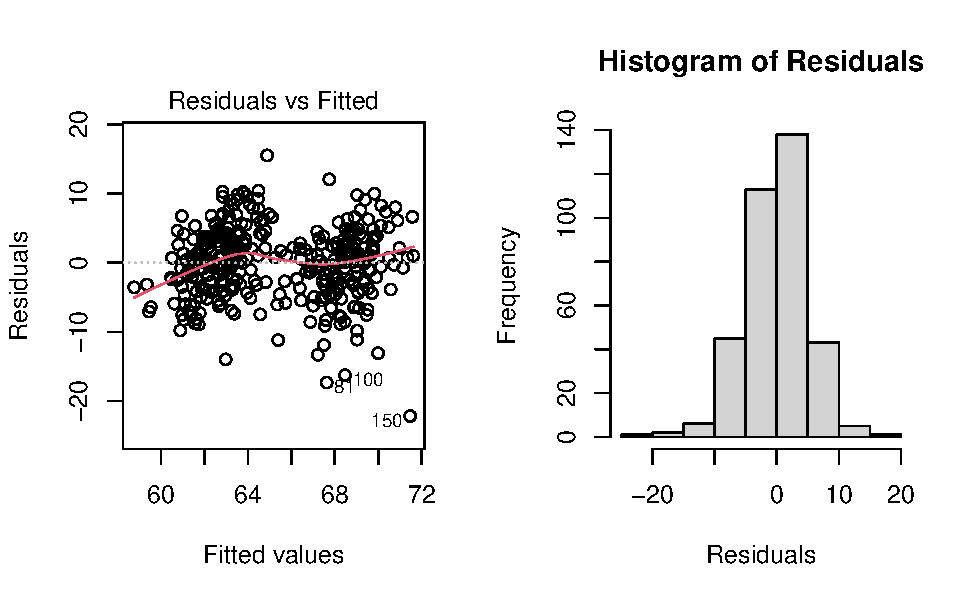
\includegraphics[width=0.5\linewidth]{03-A04-EDA-categorical_files/figure-latex/unnamed-chunk-3-1} \end{center}

\begin{enumerate}
\def\labelenumi{\arabic{enumi}.}
\setcounter{enumi}{4}
\tightlist
\item
  Which features in the relative frequency bar plot are the same as the frequency bar plot? Which are different?
\end{enumerate}

\newpage

\hypertarget{displaying-two-categorical-variables}{%
\subsubsection*{Displaying two categorical variables}\label{displaying-two-categorical-variables}}
\addcontentsline{toc}{subsubsection}{Displaying two categorical variables}

Is there an association between the level of light in a room and the development of myopia? To examine the differences in level of myopia for the level of light, we would create a segmented bar plot of \texttt{Light} segmented by \texttt{Sight}. To create the segmented bar plot enter the variable name, \texttt{Light} for \texttt{explanatory} and the variable name, \texttt{Sight} for \texttt{response} in the R script file in line 27. Highlight and run lines 26--33.

\begin{Shaded}
\begin{Highlighting}[]
\NormalTok{myopia }\SpecialCharTok{\%\textgreater{}\%} \CommentTok{\# Data set piped into...}
\FunctionTok{ggplot}\NormalTok{(}\FunctionTok{aes}\NormalTok{(}\AttributeTok{x =}\NormalTok{ explanatory, }\AttributeTok{fill =}\NormalTok{ response)) }\SpecialCharTok{+}   \CommentTok{\# This specifies the variables}
  \FunctionTok{geom\_bar}\NormalTok{(}\AttributeTok{stat =} \StringTok{"count"}\NormalTok{, }\AttributeTok{position =} \StringTok{"fill"}\NormalTok{) }\SpecialCharTok{+}  \CommentTok{\# Tell it to make a stacked bar plot}
  \FunctionTok{labs}\NormalTok{(}\AttributeTok{title =} \StringTok{"Segmented Bar Plot of Night Light Use by Level of Myopia"}\NormalTok{,  }
       \CommentTok{\# Make sure to title your plot }
       \AttributeTok{x =} \StringTok{"Level of Light"}\NormalTok{,   }\CommentTok{\# Label the x axis}
       \AttributeTok{y =} \StringTok{""}\NormalTok{) }\SpecialCharTok{+}  \CommentTok{\# Remove y axis label}
    \FunctionTok{scale\_fill\_grey}\NormalTok{()  }\CommentTok{\# Make figure black and white}
\end{Highlighting}
\end{Shaded}

\begin{enumerate}
\def\labelenumi{\arabic{enumi}.}
\setcounter{enumi}{5}
\tightlist
\item
  Sketch the segmented bar plot created here. Be sure to label the axes.
\end{enumerate}

\vspace{2in}

\begin{enumerate}
\def\labelenumi{\arabic{enumi}.}
\setcounter{enumi}{6}
\tightlist
\item
  From the segmented bar plot, estimate the proportion of no myopia for those that used a nightlight.
\end{enumerate}

\vspace{0.5in}

\begin{enumerate}
\def\labelenumi{\arabic{enumi}.}
\setcounter{enumi}{7}
\tightlist
\item
  Which level of light has the highest proportion of \texttt{No\ Myopia}?
\end{enumerate}

\vspace{0.5in}

We could also plot the data using a mosaic plot. Fill in the variable name, \texttt{Light} for \texttt{explanatory} and the variable name, \texttt{Sight} for \texttt{response} in line 38 in the R script file. Highlight and run lines 36--43.

\begin{Shaded}
\begin{Highlighting}[]
\NormalTok{myopia }\SpecialCharTok{\%\textgreater{}\%} \CommentTok{\# Data set piped into...}
  \FunctionTok{ggplot}\NormalTok{() }\SpecialCharTok{+}   \CommentTok{\# This specifies the variables}
  \FunctionTok{geom\_mosaic}\NormalTok{(}\FunctionTok{aes}\NormalTok{(}\AttributeTok{x=}\FunctionTok{product}\NormalTok{(explanatory), }\AttributeTok{fill =}\NormalTok{ response)) }\SpecialCharTok{+}  \CommentTok{\# Tell it to make a mosaic plot}
  \FunctionTok{labs}\NormalTok{(}\AttributeTok{title =} \StringTok{"Mosaic Plot of Night Light Use by Level of Myopia"}\NormalTok{,  }
       \CommentTok{\# Make sure to title your plot }
       \AttributeTok{x =} \StringTok{"Level of Light"}\NormalTok{,   }\CommentTok{\# Label the x axis}
       \AttributeTok{y =} \StringTok{""}\NormalTok{) }\SpecialCharTok{+}  \CommentTok{\# Remove y axis label}
      \FunctionTok{scale\_fill\_grey}\NormalTok{()  }\CommentTok{\# Make figure black and white}
\end{Highlighting}
\end{Shaded}

\begin{enumerate}
\def\labelenumi{\arabic{enumi}.}
\setcounter{enumi}{8}
\tightlist
\item
  What is similar and what is different between the segmented bar chart and the mosaic bar chart?
\end{enumerate}

\vspace{1in}

\begin{enumerate}
\def\labelenumi{\arabic{enumi}.}
\setcounter{enumi}{9}
\tightlist
\item
  Explain why the bar for \texttt{Nightlight} is the widest in the mosaic plot.
\end{enumerate}

\vspace{0.8in}

Fill in the name of the explanatory variable and the response variable in line 46 in the R script file, highlight and run line 46 to get the counts for each combination of levels of variables.

\begin{Shaded}
\begin{Highlighting}[]
\NormalTok{myopia }\SpecialCharTok{\%\textgreater{}\%} \FunctionTok{group\_by}\NormalTok{(explanatory) }\SpecialCharTok{\%\textgreater{}\%} \FunctionTok{count}\NormalTok{(response)}
\end{Highlighting}
\end{Shaded}

\begin{enumerate}
\def\labelenumi{\arabic{enumi}.}
\setcounter{enumi}{10}
\tightlist
\item
  Fill in the following table with the values from the R output.
\end{enumerate}

\begin{center}
\begingroup
\setlength{\tabcolsep}{14pt} % Default value: 6pt
\renewcommand{\arraystretch}{2} % Default value: 1
\begin{tabular}{|c|c|c|c|c|}
\hline
 & \multicolumn{3}{|c|}{\textbf{Light Level}} & \\ \hline
\textbf{Myopia Level} & Full Light & Nightlight & No Light & Total \\ \hline
 High Myopia & & & & \\ \hline
 Myopia & & & & \\ \hline
 No Myopia & & & & \\ \hline
 Total & & & & \\ \hline  
\end{tabular}
\endgroup
\end{center}

In the following questions, use the table to calculate the described proportions. Notation is important for each calculation. Since this is sample data it is appropriate to use statistic notation for the proportion, \(\hat{p}\). When calculating a proportion dependent on a single level of a variable subscripts are needed when reporting the notation.

\begin{enumerate}
\def\labelenumi{\arabic{enumi}.}
\setcounter{enumi}{11}
\item
  Calculate the proportion of children with high myopia. Use appropriate notation.
  \vspace{0.3in}
\item
  Calculate the proportion of children with high myopia among those that slept with full light. Use appropriate notation.
  \vspace{0.3in}
\item
  Calculate the proportion of children with high myopia among those that slept with no light. Use appropriate notation.
  \vspace{0.3in}
\item
  Calculate the difference in proportion of children with high myopia for those that slept with full light minus those who slept with no light. Give the appropriate notation. Use full light minus no light as the order of subtraction.
  \vspace{0.3in}
\end{enumerate}

\hypertarget{take-home-messages-5}{%
\subsection{Take-home messages}\label{take-home-messages-5}}

\begin{enumerate}
\def\labelenumi{\arabic{enumi}.}
\item
  Bar charts can be used to graphically display a single categorical variable either as counts or proportions. Segmented bar charts and mosaic plots are used to display two categorical variables.
\item
  Segmented bar charts always have a scale from 0 - 100\%. The bars represent the outcomes of the explanatory variable. Each bar is segmented by the response variable. If the heights of each segment are the same for each bar there is no association between variables.
\item
  Mosaic plots are similar to segmented bar charts but the widths of the bars also show the number of observations within each outcome.
\end{enumerate}

\hypertarget{additional-notes-5}{%
\subsection{Additional notes}\label{additional-notes-5}}

Use this space to summarize your thoughts and take additional notes on today's activity and material covered.

\newpage

\hypertarget{activity-3b-imdb-movie-reviews-displaying-quantitative-variables}{%
\section{Activity 3B: IMDb Movie Reviews --- Displaying Quantitative Variables}\label{activity-3b-imdb-movie-reviews-displaying-quantitative-variables}}

\setstretch{1}

\hypertarget{learning-outcomes-6}{%
\subsection{Learning outcomes}\label{learning-outcomes-6}}

\begin{itemize}
\item
  Identify and create appropriate summary statistics and plots
  given a data set or research question for quantitative data.
\item
  Interpret the following summary statistics in context:
  median, lower quartile, upper quartile,
  standard deviation, interquartile range.
\end{itemize}

\hypertarget{terminology-review-6}{%
\subsection{Terminology review}\label{terminology-review-6}}

In today's activity, we will review summary measures and plots for quantitative variables. Some terms covered in this activity are:

\begin{itemize}
\item
  Two measures of center: mean, median
\item
  Two measures of spread (variability): standard deviation, interquartile range (IQR)
\item
  Types of graphs: box plots, dot plots, histograms
\item
  Identify and create appropriate summary statistics and plots given a data set or research question for a single categorical and a single quantitative variable.
\item
  Interpret the following summary statistics in context:
  median, lower quartile, upper quartile,
  standard deviation, interquartile range.
\item
  Given a plot or set of plots, describe and compare the distribution(s)
  of a single quantitative variable
  (center, variability, shape, outliers).
\end{itemize}

To review these concepts, see Section 2.3 in the textbook.

\hypertarget{movies-released-in-2016}{%
\subsection{Movies released in 2016}\label{movies-released-in-2016}}

A data set was collected on movies released in 2016 ({``{IMDb} Movies Extensive Dataset''} 2016). Here is a list of some of the variables collected on the observational units, movies released in 2016.

\begin{longtable}[]{@{}
  >{\raggedright\arraybackslash}p{(\columnwidth - 2\tabcolsep) * \real{0.2353}}
  >{\raggedright\arraybackslash}p{(\columnwidth - 2\tabcolsep) * \real{0.7647}}@{}}
\toprule()
\begin{minipage}[b]{\linewidth}\raggedright
\textbf{Variable}
\end{minipage} & \begin{minipage}[b]{\linewidth}\raggedright
\textbf{Description}
\end{minipage} \\
\midrule()
\endhead
\texttt{budget\_mil} & Amount of money (in US \$ millions) budgeted for the production of the movie \\
\texttt{revenue\_mil} & Amount of money (in US \$ millions) the movie made after release \\
\texttt{duration} & Length of the movie (in minutes) \\
\texttt{content\_rating} & Rating of the movie (\texttt{G}, \texttt{PG}, \texttt{PG-13}, \texttt{R}, \texttt{Not\ Rated}) \\
\texttt{imdb\_score} & IMDb user rating score from 1 to 10 \\
\texttt{genres} & Categories the movie falls into (e.g., Action, Drama, etc.) \\
\texttt{facebook\_likes} & Number of likes a movie receives on Facebook \\
\bottomrule()
\end{longtable}

\newpage

\hypertarget{summarizing-a-single-quantitative-variable}{%
\subsubsection*{Summarizing a single quantitative variable}\label{summarizing-a-single-quantitative-variable}}
\addcontentsline{toc}{subsubsection}{Summarizing a single quantitative variable}

The \texttt{favstats()} function from the \texttt{mosaic} package gives the summary statistics for a quantitative variable. Here we have the summary statistics for the variable \texttt{imdb\_score}. The summary statistics give the two measures of center and two measures of spread for IMDb score. Highlight and run lines 1 -- 8 in the provided \texttt{R} script file to load the data set. Check that the summary statistics match that printed in the coursepack.

\begin{Shaded}
\begin{Highlighting}[]
\CommentTok{\# Read in data set}
\NormalTok{movies }\OtherTok{\textless{}{-}} \FunctionTok{read.csv}\NormalTok{(}\StringTok{"https://math.montana.edu/courses/s216/data/Movies2016.csv"}\NormalTok{) }
\NormalTok{movies }\SpecialCharTok{\%\textgreater{}\%} \CommentTok{\# Data set piped into...}
  \FunctionTok{summarise}\NormalTok{(}\FunctionTok{favstats}\NormalTok{(imdb\_score)) }\CommentTok{\# Apply favstats function to imdb\_score}
\end{Highlighting}
\end{Shaded}

\begin{verbatim}
#>   min   Q1 median  Q3 max     mean       sd  n missing
#> 1 3.4 5.65    6.4 7.1 8.2 6.309783 1.086689 92       0
\end{verbatim}

\begin{enumerate}
\def\labelenumi{\arabic{enumi}.}
\tightlist
\item
  Give the values for the two measures of center (mean and median).
\end{enumerate}

\vspace{0.5in}

\begin{enumerate}
\def\labelenumi{\arabic{enumi}.}
\setcounter{enumi}{1}
\tightlist
\item
  Report the value for quartile 1 and interpret this value in context of the problem.
\end{enumerate}

\vspace{0.5in}

\begin{enumerate}
\def\labelenumi{\arabic{enumi}.}
\setcounter{enumi}{2}
\tightlist
\item
  Calculate the interquartile range (IQR = Q3 - Q1).
\end{enumerate}

\vspace{0.5in}

\begin{enumerate}
\def\labelenumi{\arabic{enumi}.}
\setcounter{enumi}{3}
\tightlist
\item
  Report the value of the standard deviation and interpret this value in context of the problem.
  \vspace{0.8in}
\end{enumerate}

\hypertarget{displaying-a-single-quantitative-variable}{%
\subsubsection*{Displaying a single quantitative variable}\label{displaying-a-single-quantitative-variable}}
\addcontentsline{toc}{subsubsection}{Displaying a single quantitative variable}

\begin{enumerate}
\def\labelenumi{\arabic{enumi}.}
\setcounter{enumi}{4}
\tightlist
\item
  What are the three types of plots used to plot a single quantitative variable?
\end{enumerate}

\newpage

A dotplot will plot a dot for each value in the data set. The following code will create a dotplot of IMDb scores. Notice that we put in the variable name \texttt{imdb\_score} for \texttt{x\ =} in the ggplot function.

\begin{Shaded}
\begin{Highlighting}[]
\NormalTok{movies }\SpecialCharTok{\%\textgreater{}\%} \CommentTok{\# Data set piped into...}
\FunctionTok{ggplot}\NormalTok{(}\FunctionTok{aes}\NormalTok{(}\AttributeTok{x =}\NormalTok{ imdb\_score)) }\SpecialCharTok{+}   \CommentTok{\# Name variable to plot}
  \FunctionTok{geom\_dotplot}\NormalTok{() }\SpecialCharTok{+}  \CommentTok{\# Create dotplot}
  \FunctionTok{labs}\NormalTok{(}\AttributeTok{title =} \StringTok{"Dotplot of IMDb Score of Movies in 2016"}\NormalTok{, }\CommentTok{\# Title for plot}
       \AttributeTok{x =} \StringTok{"IMDb Score"}\NormalTok{, }\CommentTok{\# Label for x axis}
       \AttributeTok{y =} \StringTok{"Frequency"}\NormalTok{) }\CommentTok{\# Label for y axis}
\end{Highlighting}
\end{Shaded}

\begin{center}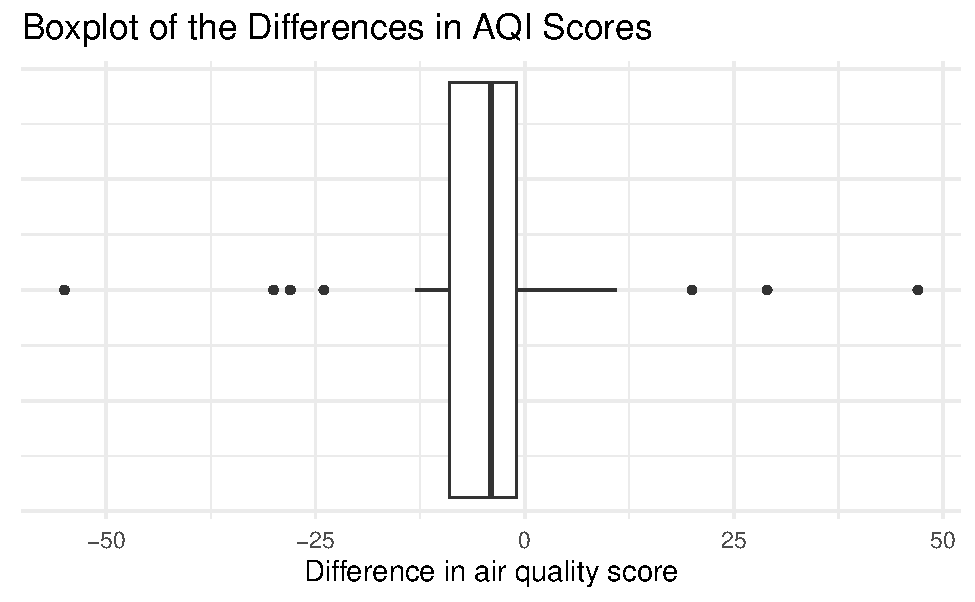
\includegraphics[width=0.6\linewidth]{03-A05-EDA-quantitative_files/figure-latex/unnamed-chunk-2-1} \end{center}

\begin{enumerate}
\def\labelenumi{\arabic{enumi}.}
\setcounter{enumi}{5}
\tightlist
\item
  What is the shape of the distribution of IMDb scores?
\end{enumerate}

\vspace{0.2in}

To create a histogram of the IMDb scores, enter the variable name, \texttt{imdb\_score} in the provided \texttt{R} script file for \texttt{variable} at line 20, highlight and run lines 19--24. Visually, this shows us the range of IMDb scores for Movies released in 2016.

Notice that the \textbf{bin width} is 0.5. For example the first bin consists of the number of movies in the data set with an IMDb score of 3.25 to 3.75. It is important to note that a movie with a IMDb score on the boundary of a bin will fall into the bin above it; for example, 4.75 would be counted in the bin 4.75--5.25.

\begin{Shaded}
\begin{Highlighting}[]
\NormalTok{movies }\SpecialCharTok{\%\textgreater{}\%} \CommentTok{\# Data set piped into...}
\FunctionTok{ggplot}\NormalTok{(}\FunctionTok{aes}\NormalTok{(}\AttributeTok{x =}\NormalTok{ variable)) }\SpecialCharTok{+}   \CommentTok{\# Name variable to plot}
  \FunctionTok{geom\_histogram}\NormalTok{(}\AttributeTok{binwidth =} \FloatTok{0.5}\NormalTok{) }\SpecialCharTok{+}  \CommentTok{\# Create histogram with specified binwidth}
  \FunctionTok{labs}\NormalTok{(}\AttributeTok{title =} \StringTok{"Histogram of IMDb Score of Movies in 2016"}\NormalTok{, }\CommentTok{\# Title for plot}
       \AttributeTok{x =} \StringTok{"IMDb Score"}\NormalTok{, }\CommentTok{\# Label for x axis}
       \AttributeTok{y =} \StringTok{"Frequency"}\NormalTok{) }\CommentTok{\# Label for y axis}
\end{Highlighting}
\end{Shaded}

\begin{enumerate}
\def\labelenumi{\arabic{enumi}.}
\setcounter{enumi}{6}
\tightlist
\item
  Sketch the histogram created here.
\end{enumerate}

\vspace{1.4in}

\begin{enumerate}
\def\labelenumi{\arabic{enumi}.}
\setcounter{enumi}{7}
\tightlist
\item
  Which range of IMDb scores have the highest frequency?
\end{enumerate}

\vspace{0.2in}

To create a boxplot of the IMDb scores, enter the variable name, \texttt{imdb\_score} in the provided \texttt{R} script file for \texttt{variable} at line 28, highlight and run lines 27--32. Visually, this shows us the range of IMDb scores for Movies released in 2016.

\begin{Shaded}
\begin{Highlighting}[]
\NormalTok{movieS }\SpecialCharTok{\%\textgreater{}\%} \CommentTok{\# Data set piped into...}
\FunctionTok{ggplot}\NormalTok{(}\FunctionTok{aes}\NormalTok{(}\AttributeTok{x =}\NormalTok{ variable)) }\SpecialCharTok{+}   \CommentTok{\# Name variable to plot}
  \FunctionTok{geom\_boxplot}\NormalTok{() }\SpecialCharTok{+}  \CommentTok{\# Create boxplot }
  \FunctionTok{labs}\NormalTok{(}\AttributeTok{title =} \StringTok{"Boxplot of IMDb Score of Movies in 2016"}\NormalTok{, }\CommentTok{\# Title for plot}
       \AttributeTok{x =} \StringTok{"IMDb Score"}\NormalTok{, }\CommentTok{\# Label for x axis}
       \AttributeTok{y =} \StringTok{"Frequency"}\NormalTok{) }\CommentTok{\# Label for y axis}
\end{Highlighting}
\end{Shaded}

\begin{enumerate}
\def\labelenumi{\arabic{enumi}.}
\setcounter{enumi}{8}
\tightlist
\item
  Sketch the boxplot created and identify the values of the 5-number summary (minimum value, first quartile (\(Q_1\)), median, third quartile (\(Q_3\)), maximum value) on the plot. Use the following formulas to find the invisible fence on both ends of the distribution. Draw a dotted line at the invisible fence to show how the outliers were found.
\end{enumerate}

\[\text{Lower Fence: values} \le Q_1 - 1.5\times IQR\]

\[\text{Upper Fence: values} \ge Q_3 + 1.5\times IQR\]
\vspace{2in}

\begin{enumerate}
\def\labelenumi{\arabic{enumi}.}
\setcounter{enumi}{9}
\item
  Compare the three graphs of IMDb scores created above.

  Which graph is best used to show the shape of the distribution?

  \vspace{0.5in}

  Which graph is best used to show the outliers of the distribution?

  \vspace{0.5in}
\end{enumerate}

\hypertarget{summary-statistics-for-a-single-categorical-and-single-quantitative-variable}{%
\subsubsection*{Summary statistics for a single categorical and single quantitative Variable}\label{summary-statistics-for-a-single-categorical-and-single-quantitative-variable}}
\addcontentsline{toc}{subsubsection}{Summary statistics for a single categorical and single quantitative Variable}

Is there an association between content rating and budget for movies in 2016? To use the \texttt{favstats()} function in the mosaic package with two variables, we will enter the variables as a formula, response\textasciitilde explanatory. This function will give the summary statistics for budget for each content rating. Highlight and run lines 35--37 in the provided \texttt{R} script file and check that the summary statistics match those provided in the coursepack.

\begin{Shaded}
\begin{Highlighting}[]
\NormalTok{movies }\SpecialCharTok{\%\textgreater{}\%} \CommentTok{\# Data set piped into...}
  \FunctionTok{filter}\NormalTok{(content\_rating }\SpecialCharTok{!=} \StringTok{"Not Rated"}\NormalTok{) }\SpecialCharTok{\%\textgreater{}\%} \CommentTok{\# Remove Not Rated movies}
  \FunctionTok{summarise}\NormalTok{(}\FunctionTok{favstats}\NormalTok{(budget\_mil}\SpecialCharTok{\textasciitilde{}}\NormalTok{content\_rating)) }\CommentTok{\# Find the summary measures for each content rating}
\end{Highlighting}
\end{Shaded}

\begin{verbatim}
#>   content_rating min    Q1 median      Q3 max     mean       sd  n missing
#> 1             PG 0.5 11.00   74.0 151.250 175 86.54167 71.52795 12       0
#> 2          PG-13 0.0 17.25   33.5 138.750 250 74.17500 74.15190 46       0
#> 3              R 0.0  7.75   19.5  29.625  60 21.09375 16.99926 32       0
\end{verbatim}

\begin{enumerate}
\def\labelenumi{\arabic{enumi}.}
\setcounter{enumi}{10}
\tightlist
\item
  Which content rating has the largest IQR?
\end{enumerate}

\vspace{0.8in}

\begin{enumerate}
\def\labelenumi{\arabic{enumi}.}
\setcounter{enumi}{11}
\tightlist
\item
  Report the mean budget amount for the PG rating. Use appropriate notation.
\end{enumerate}

\vspace{0.3in}

\begin{enumerate}
\def\labelenumi{\arabic{enumi}.}
\setcounter{enumi}{12}
\tightlist
\item
  Report the mean budget amount for the R rating. Use appropriate notation.
\end{enumerate}

\vspace{0.3in}

\begin{enumerate}
\def\labelenumi{\arabic{enumi}.}
\setcounter{enumi}{13}
\tightlist
\item
  Calculate the difference in mean budget amount for movies in 2016 with a PG rating minus those with a R rating. Use appropriate notation with informative subscripts.
\end{enumerate}

\vspace{0.8in}

\newpage

\hypertarget{displaying-a-single-categorical-and-single-quantitative-variable}{%
\subsubsection*{Displaying a single categorical and single quantitative variable}\label{displaying-a-single-categorical-and-single-quantitative-variable}}
\addcontentsline{toc}{subsubsection}{Displaying a single categorical and single quantitative variable}

The boxplot of movie budgets (in millions) by content rating is plotted using the code below. Enter the variable \texttt{budget\_mil} for \texttt{response} and the variable \texttt{content\_rating} for explanatory at line 42, highlight and run code lines 40--46. This plot compares the budget for different levels of content rating.

\begin{Shaded}
\begin{Highlighting}[]
\NormalTok{movies }\SpecialCharTok{\%\textgreater{}\%}  \CommentTok{\# Data set piped into...}
  \FunctionTok{filter}\NormalTok{(content\_rating }\SpecialCharTok{!=} \StringTok{"Not Rated"}\NormalTok{) }\SpecialCharTok{\%\textgreater{}\%} \CommentTok{\# Remove Not Rated movies}
  \FunctionTok{ggplot}\NormalTok{(}\FunctionTok{aes}\NormalTok{(}\AttributeTok{y =}\NormalTok{ response, }\AttributeTok{x =}\NormalTok{ explanatory))}\SpecialCharTok{+}  \CommentTok{\# Identify variables}
  \FunctionTok{geom\_boxplot}\NormalTok{()}\SpecialCharTok{+}  \CommentTok{\# Tell it to make a box plot}
  \FunctionTok{labs}\NormalTok{(}\AttributeTok{title =} \StringTok{"Side by side box plot of budget by content rating"}\NormalTok{,  }\CommentTok{\# Title}
       \AttributeTok{x =} \StringTok{"Content Rating"}\NormalTok{,    }\CommentTok{\# x{-}axis label}
       \AttributeTok{y =} \StringTok{"Budget (in Millions)"}\NormalTok{)  }\CommentTok{\# y{-}axis label}
\end{Highlighting}
\end{Shaded}

\begin{enumerate}
\def\labelenumi{\arabic{enumi}.}
\setcounter{enumi}{14}
\tightlist
\item
  Sketch the box plots created using the \texttt{R} code.
\end{enumerate}

\vspace{1.5in}

\begin{enumerate}
\def\labelenumi{\arabic{enumi}.}
\setcounter{enumi}{15}
\tightlist
\item
  Answer the following questions about the box plots created.
\end{enumerate}

\begin{enumerate}
\def\labelenumi{\alph{enumi}.}
\item
  Which content rating has the highest center?
  \vspace{0.2in}
\item
  Which content rating has the largest spread?
  \vspace{0.2in}
\item
  Which content rating has the most skewed distribution?
  \vspace{0.2in}
\item
  Fifty percent of movies in 2016 with a PG-13 content rating fall below what value? What is the name of this value?
  \vspace{0.4in}
\end{enumerate}

\begin{enumerate}
\def\labelenumi{\arabic{enumi}.}
\setcounter{enumi}{16}
\tightlist
\item
  Which variable is the explanatory variable? Response variable?
\end{enumerate}

\vspace{0.4in}

\newpage

\hypertarget{take-home-messages-6}{%
\subsection{Take-home messages}\label{take-home-messages-6}}

\begin{enumerate}
\def\labelenumi{\arabic{enumi}.}
\item
  Histograms, box plots, and dot plots can all be used to graphically display a single quantitative variable.
\item
  The box plot is created using the five number summary: minimum value, quartile 1, median, quartile 3, and maximum value. Values in the data set that are less than \(Q_1 - 1.5\times IQR\) and greater than \(Q_3 + 1.5\times IQR\) are considered outliers and are graphically represented by a dot outside of the whiskers on the box plot.
\item
  Data should be summarized numerically and displayed graphically to give us information about the study.
\item
  When comparing distributions of quantitative variables we look at the shape, center, spread, and for outliers. There are two measures of center: mean and the median and two measures of spread: standard deviation and the interquartile range, \(IQR = Q_3 - Q_1\).
\end{enumerate}

\hypertarget{additional-notes-6}{%
\subsection{Additional notes}\label{additional-notes-6}}

Use this space to summarize your thoughts and take additional notes on today's activity and material covered.

\newpage

\hypertarget{week-3-lab-ipeds}{%
\section{Week 3 Lab: IPEDs}\label{week-3-lab-ipeds}}

\setstretch{1}

\hypertarget{learning-outcomes-7}{%
\subsection{Learning outcomes}\label{learning-outcomes-7}}

\begin{itemize}
\item
  Identify and create appropriate summary statistics and plots
  given a data set or research question for quantitative data.
\item
  Interpret the following summary statistics in context:
  median, lower quartile, upper quartile,
  standard deviation, interquartile range.
\end{itemize}

\hypertarget{terminology-review-7}{%
\subsection{Terminology review}\label{terminology-review-7}}

In today's lab, we will review summary measures and plots for quantitative variables. Some terms covered in this activity are:

\begin{itemize}
\item
  Two measures of center: mean, median
\item
  Two measures of spread (variability): standard deviation, interquartile range (\(IQR\))
\item
  Types of graphs: box plots, dot plots, histograms
\item
  Identify and create appropriate summary statistics and plots given a data set or research question for a single categorical and a single quantitative variable.
\item
  Interpret the following summary statistics in context:
  median, lower quartile, upper quartile,
  standard deviation, interquartile range.
\item
  Given a plot or set of plots, describe and compare the distribution(s)
  of a single quantitative variable
  (center, variability, shape, outliers).
\end{itemize}

To review these concepts, see Chapter 5 in the textbook.

\hypertarget{the-integrated-postsecondary-education-data-system-ipeds}{%
\subsection{The Integrated Postsecondary Education Data System (IPEDS)}\label{the-integrated-postsecondary-education-data-system-ipeds}}

Upload and open the provided R script file for the week 3 lab to answer the following questions. \textbf{Remember bolded questions will be answered on Gradescope for your group.}

These data are on a subset of institutions that met the following selection criteria (Education Statistics 2018):

\begin{itemize}
\item
  Degree granting
\item
  United States only
\item
  Title IV participating
\item
  Not for profit
\item
  2-year or 4-year or above
\item
  Has full-time first-time undergraduates
\item
  Note that several variables have missing values for some institutions (denoted by ``NA'').
\end{itemize}

\begin{center}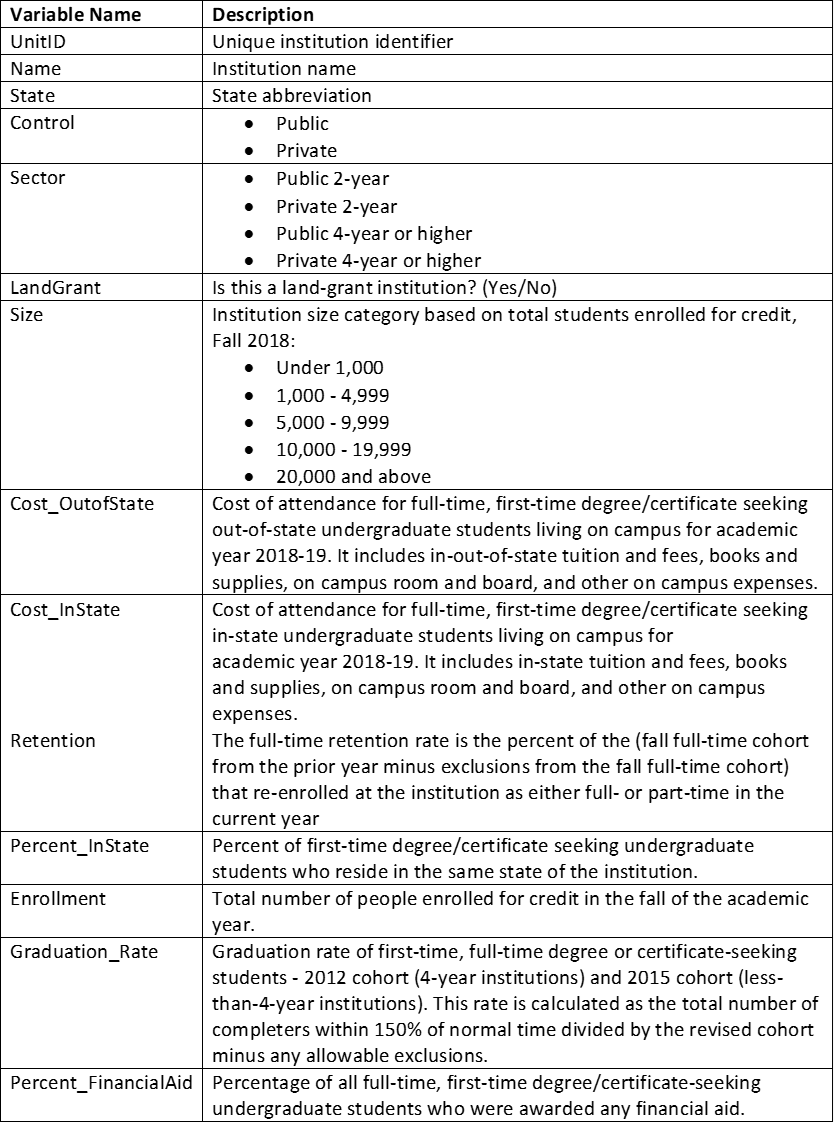
\includegraphics[width=0.75\linewidth]{images/IPEDS_Description} \end{center}

\hypertarget{summary-statistics-for-a-single-quantitative-variable}{%
\subsubsection*{Summary statistics for a single quantitative variable}\label{summary-statistics-for-a-single-quantitative-variable}}
\addcontentsline{toc}{subsubsection}{Summary statistics for a single quantitative variable}

Look through the provided chart above showing the description of variables measured. The UnitID and Name are identifiers for each observational unit, \emph{US degree granting institutions in 2018}.

\begin{enumerate}
\def\labelenumi{\arabic{enumi}.}
\tightlist
\item
  Identify in the chart above which variables collected on the US institutions are categorical (C) and which variables are quantitative (Q).
\end{enumerate}

\newpage

In Wednesday's activity, the code was provided to import the data set needed directly from the Stat 216 website. Follow these steps to upload and import the data set for today's lab.

\begin{itemize}
\item
  Download the provided data set \texttt{IPEDS\_Data\_2018} from D2L
\item
  Upload the data set \texttt{IPEDS\_Data\_2018} to the RStudio server using the same steps to upload the R script file.
\item
  Click on ``Import Dataset'' in the Environment tab in the upper right hand corner.
\item
  Choose ``From Text(base)'' in the drop-down menu and select the correct csv file.
\item
  Be sure that ``Yes'' is selected next to ``Heading'' in the pop-up screen. Click ``Import''.
\item
  To view the data set, click on the data set name (\texttt{IPEDS\_Data\_2018}). Verify that that column names match the first column in the chart on the previous page. If the columns are named V1, V2, V3\ldots etc, you did not select ``Yes'' for ``Heading''.
\end{itemize}

Enter the name of the data set (see the environment tab) for \texttt{datasetname} in the R script file in line 6. We will look at the retention rates for the 4-year institutions only. Enter the variable name \texttt{Retention} for \texttt{variable} in line 12. Highlight and run lines 1 -- 12. \textbf{Note that the two lines of code (lines 8 and 10) are filtering to remove the 2-year institutions so we are only assessing Public 4-year and Private 4-year institutions.} The \texttt{favstats()} function from the \texttt{mosaic} package gives the summary statistics for a quantitative variable. The summary statistics give the two measures of center and two measures of spread for retention rate.

\begin{Shaded}
\begin{Highlighting}[]
\NormalTok{IPEDS }\OtherTok{\textless{}{-}}\NormalTok{ datasetname }\CommentTok{\#Creates the object IPEDS }
\NormalTok{IPEDS }\OtherTok{\textless{}{-}}\NormalTok{ IPEDS }\SpecialCharTok{\%\textgreater{}\%}
  \FunctionTok{filter}\NormalTok{(Sector }\SpecialCharTok{!=} \StringTok{"Public 2{-}year"}\NormalTok{) }\CommentTok{\#Filters the data set to remove Public 2{-}year}
\NormalTok{IPEDS }\OtherTok{\textless{}{-}}\NormalTok{ IPEDS }\SpecialCharTok{\%\textgreater{}\%}
  \FunctionTok{filter}\NormalTok{(Sector }\SpecialCharTok{!=} \StringTok{"Private 2{-}year"}\NormalTok{) }\CommentTok{\#Filters the data set to remove Private 2{-}year}
\NormalTok{IPEDS }\SpecialCharTok{\%\textgreater{}\%}
  \FunctionTok{summarise}\NormalTok{(}\FunctionTok{favstats}\NormalTok{(variable)) }\CommentTok{\#Gives the summary statistics}
\end{Highlighting}
\end{Shaded}

\begin{enumerate}
\def\labelenumi{\arabic{enumi}.}
\setcounter{enumi}{1}
\tightlist
\item
  \textbf{Report the value for quartile 3 and interpret this value in context of the study.}
\end{enumerate}

\vspace{1in}

\begin{enumerate}
\def\labelenumi{\arabic{enumi}.}
\setcounter{enumi}{2}
\tightlist
\item
  Calculate the interquartile range (\(IQR = Q_3 - Q_1\)) for this study.
\end{enumerate}

\vspace{0.5in}

\begin{enumerate}
\def\labelenumi{\arabic{enumi}.}
\setcounter{enumi}{3}
\tightlist
\item
  Report and interpret the value of the standard deviation.
\end{enumerate}

\vspace{1in}

\begin{enumerate}
\def\labelenumi{\arabic{enumi}.}
\setcounter{enumi}{4}
\tightlist
\item
  How many missing values are there? What does this indicate?
\end{enumerate}

\vspace{0.8in}

\hypertarget{displaying-a-single-quantitative-variable-1}{%
\subsubsection*{Displaying a single quantitative variable}\label{displaying-a-single-quantitative-variable-1}}
\addcontentsline{toc}{subsubsection}{Displaying a single quantitative variable}

There are three type of plots used to plot a single quantitative variable: a dotplot, a histogram or a boxplot. A dotplot of retention rates would plot a dot for the retention rate for each 4-year institution.

We will create both a histogram and a boxplot of the variable \texttt{Retention}. Enter the name of the variable in both line 16 and line 23 for \texttt{variable} in the R script file. \textbf{Give each plot a descriptive title.} Highlight and run lines 15 -- 27 to give the histogram and boxplot. Notice that the \textbf{bin width} for the histogram is 10. For example, the first bin consists of the number of 4-year institutions in the data set with a retention rate of 0 to 10\%. It is important to note that a 4-year institution with a retention rate on the boundary of a bin will fall into the bin above it; for example, 10 would be counted in the bin 10--20.

\textbf{Export and upload both plots to Gradescope for your group.}

\begin{itemize}
\item
  To export the graphs: in the bottom right corner in the Plots tab, click on \texttt{Export}.
\item
  Then choose \texttt{Save\ as\ Image}. Save the image as a png. This will save your graph to the server.
\item
  In the Files tab, click on the box next to your saved image file, click \texttt{More} and choose \texttt{Export}. This will save your file to your downloads folder on your computer.
\end{itemize}

\begin{Shaded}
\begin{Highlighting}[]
\NormalTok{IPEDS }\SpecialCharTok{\%\textgreater{}\%} \CommentTok{\# Data set piped into...}
\FunctionTok{ggplot}\NormalTok{(}\FunctionTok{aes}\NormalTok{(}\AttributeTok{x =}\NormalTok{ variable)) }\SpecialCharTok{+}   \CommentTok{\# Name variable to plot}
  \FunctionTok{geom\_histogram}\NormalTok{(}\AttributeTok{binwidth =} \DecValTok{10}\NormalTok{) }\SpecialCharTok{+}  \CommentTok{\# Create histogram with specified binwidth }
  \FunctionTok{labs}\NormalTok{(}\AttributeTok{title =} \StringTok{"Title"}\NormalTok{, }\CommentTok{\# Title for plot}
       \AttributeTok{x =} \StringTok{"Rentention Rate"}\NormalTok{, }\CommentTok{\# Label for x axis}
       \AttributeTok{y =} \StringTok{"Frequency"}\NormalTok{) }\CommentTok{\# Label for y axis}
\end{Highlighting}
\end{Shaded}

\begin{Shaded}
\begin{Highlighting}[]
\NormalTok{IPEDS }\SpecialCharTok{\%\textgreater{}\%} \CommentTok{\# Data set piped into...}
\FunctionTok{ggplot}\NormalTok{(}\FunctionTok{aes}\NormalTok{(}\AttributeTok{x =}\NormalTok{ variable)) }\SpecialCharTok{+}   \CommentTok{\# Name variable to plot}
  \FunctionTok{geom\_boxplot}\NormalTok{() }\SpecialCharTok{+}  \CommentTok{\# Create boxplot }
  \FunctionTok{labs}\NormalTok{(}\AttributeTok{title =} \StringTok{"Title"}\NormalTok{, }\CommentTok{\# Title for plot}
       \AttributeTok{x =} \StringTok{"Retention Rates"}\NormalTok{, }\CommentTok{\# Label for x axis}
       \AttributeTok{y =} \StringTok{"Frequency"}\NormalTok{) }\CommentTok{\# Label for y axis}
\end{Highlighting}
\end{Shaded}

\begin{enumerate}
\def\labelenumi{\arabic{enumi}.}
\setcounter{enumi}{5}
\tightlist
\item
  What is the shape of the distribution of retention rates?
\end{enumerate}

\vspace{0.2in}

\begin{enumerate}
\def\labelenumi{\arabic{enumi}.}
\setcounter{enumi}{6}
\tightlist
\item
  Identify any outliers in the data set.
\end{enumerate}

\vspace{0.3in}

\hypertarget{robust-statistics}{%
\subsubsection*{Robust Statistics}\label{robust-statistics}}
\addcontentsline{toc}{subsubsection}{Robust Statistics}

Let's examine how the presence of outliers affect the values of center and spread.

\begin{enumerate}
\def\labelenumi{\arabic{enumi}.}
\setcounter{enumi}{7}
\tightlist
\item
  Report the two measures of center (mean and median) for retention given in the R output.
\end{enumerate}

\vspace{0.4in}

\begin{enumerate}
\def\labelenumi{\arabic{enumi}.}
\setcounter{enumi}{8}
\tightlist
\item
  Report the two measures of spread (standard deviation and \(IQR\)) for retention given in the R output.
\end{enumerate}

\vspace{0.4in}

To show the effect of outliers on the measures of center and spread, the smallest values of retention rate in the data set were increased by 30\%. Highlight and run lines 30--38.

\begin{Shaded}
\begin{Highlighting}[]
\NormalTok{IPEDS }\SpecialCharTok{\%\textgreater{}\%} \CommentTok{\# Data set piped into...}
  \FunctionTok{summarise}\NormalTok{(}\FunctionTok{favstats}\NormalTok{(Retention\_Inc))}
\end{Highlighting}
\end{Shaded}

\begin{Shaded}
\begin{Highlighting}[]
\NormalTok{IPEDS }\SpecialCharTok{\%\textgreater{}\%} \CommentTok{\# Data set piped into...}
  \FunctionTok{ggplot}\NormalTok{(}\FunctionTok{aes}\NormalTok{(}\AttributeTok{x =}\NormalTok{ Retention\_Inc)) }\SpecialCharTok{+}   \CommentTok{\# Name variable to plot}
  \FunctionTok{geom\_boxplot}\NormalTok{() }\SpecialCharTok{+}  \CommentTok{\# Create histogram with specified binwidth}
  \FunctionTok{labs}\NormalTok{(}\AttributeTok{title =} \StringTok{"Boxplot of Retention Rates for US Higher Education Institutions"}\NormalTok{, }\CommentTok{\# Title for plot}
       \AttributeTok{x =} \StringTok{"Retention Rate"}\NormalTok{, }\CommentTok{\# Label for x axis}
       \AttributeTok{y =} \StringTok{"Frequency"}\NormalTok{) }\CommentTok{\# Label for y axis}
\end{Highlighting}
\end{Shaded}

\begin{enumerate}
\def\labelenumi{\arabic{enumi}.}
\setcounter{enumi}{9}
\tightlist
\item
  Report the two measures of center for this new data set.
\end{enumerate}

\vspace{0.8in}

\begin{enumerate}
\def\labelenumi{\arabic{enumi}.}
\setcounter{enumi}{10}
\tightlist
\item
  Report the two measures of spread for this new data set.
\end{enumerate}

\vspace{0.8in}

\begin{enumerate}
\def\labelenumi{\arabic{enumi}.}
\setcounter{enumi}{11}
\tightlist
\item
  \textbf{Which measure of center is robust to (not affected by) outliers? Explain your answer.}
\end{enumerate}

\vspace{0.5in}

\begin{enumerate}
\def\labelenumi{\arabic{enumi}.}
\setcounter{enumi}{12}
\tightlist
\item
  Which measure of spread is robust to outliers? Explain your answer.
\end{enumerate}

\vspace{0.5in}

\hypertarget{summarizing-a-single-categorical-and-single-quantitative-variable}{%
\subsubsection*{Summarizing a single categorical and single quantitative variable}\label{summarizing-a-single-categorical-and-single-quantitative-variable}}
\addcontentsline{toc}{subsubsection}{Summarizing a single categorical and single quantitative variable}

Is there a difference in retention rates for public and private 4-year institutions? In the next part of the activity we will compare retention rates for public and private 4-year institutions. Note that this variable (public or private) is labelled \texttt{Control} in the data set.

\begin{enumerate}
\def\labelenumi{\arabic{enumi}.}
\setcounter{enumi}{13}
\tightlist
\item
  \textbf{Based on the research question, which variable will we treat as the explanatory variable? Response variable?}
\end{enumerate}

\vspace{0.8in}

Enter the name of the explanatory variable and the name of the response variable in lines 42 and 45 of the R script file. Remember that the variable name must be typed in EXACTLY as it is written in the data set. Highlight and run lines 41 -- 49 to find the summary statistics and create side by side boxplots of the data.

\begin{Shaded}
\begin{Highlighting}[]
\NormalTok{IPEDS }\SpecialCharTok{\%\textgreater{}\%}  \CommentTok{\# Data set piped into...}
  \FunctionTok{summarise}\NormalTok{(}\FunctionTok{favstats}\NormalTok{(response}\SpecialCharTok{\textasciitilde{}}\NormalTok{explanatory)) }\CommentTok{\# Summary statistics for retention rates by sector}
\end{Highlighting}
\end{Shaded}

\begin{Shaded}
\begin{Highlighting}[]
\NormalTok{IPEDS }\SpecialCharTok{\%\textgreater{}\%}  \CommentTok{\# Data set piped into...}
  \FunctionTok{ggplot}\NormalTok{(}\FunctionTok{aes}\NormalTok{(}\AttributeTok{y =}\NormalTok{ response, }\AttributeTok{x =}\NormalTok{ explanatory))}\SpecialCharTok{+}  \CommentTok{\# Identify variables}
  \FunctionTok{geom\_boxplot}\NormalTok{()}\SpecialCharTok{+}  \CommentTok{\# Create box plot}
  \FunctionTok{labs}\NormalTok{(}\AttributeTok{title =} \StringTok{"Side by side box plot of retention rates by control"}\NormalTok{,  }\CommentTok{\# Title}
       \AttributeTok{x =} \StringTok{"Control"}\NormalTok{,    }\CommentTok{\# x{-}axis label}
       \AttributeTok{y =} \StringTok{"Retention Rates"}\NormalTok{)  }\CommentTok{\# y{-}axis label}
\end{Highlighting}
\end{Shaded}

\begin{enumerate}
\def\labelenumi{\arabic{enumi}.}
\setcounter{enumi}{14}
\item
  \textbf{Compare the two boxplots.}

  Which type of university has the highest center?
  \vspace{0.3in}

  Largest spread?
  \vspace{0.3in}

  What is the shape of each distribution?
  \vspace{0.3in}

  Does either distribution have outliers?
  \vspace{0.3in}
\item
  Report the difference in mean retention rates for private and public universities. Use private minus public as the order of subtraction. Use the appropriate notation.
\end{enumerate}

\vspace{0.8in}

\begin{enumerate}
\def\labelenumi{\arabic{enumi}.}
\setcounter{enumi}{16}
\tightlist
\item
  Does there appear to be an association between retention rates and type of university? Explain your answer.
\end{enumerate}

\vspace{0.3in}

\hypertarget{summarizing-two-categorical-variables}{%
\subsubsection*{Summarizing two categorical variables}\label{summarizing-two-categorical-variables}}
\addcontentsline{toc}{subsubsection}{Summarizing two categorical variables}

Are private 4-year institutions smaller than public one? The following set of code will create a segmented bar plot of size of the institution by sector. Enter the variable \texttt{Sector} for explanatory and \texttt{Size} for response in line 64. Highlight and run lines 63--69 in the R script file.

\begin{Shaded}
\begin{Highlighting}[]
\NormalTok{IPEDS }\SpecialCharTok{\%\textgreater{}\%}
  \FunctionTok{ggplot}\NormalTok{(}\FunctionTok{aes}\NormalTok{(}\AttributeTok{x=}\NormalTok{explanatory, }\AttributeTok{fill =}\NormalTok{ response)) }\SpecialCharTok{+} \CommentTok{\# Enter the explanatory and response variables}
  \FunctionTok{geom\_bar}\NormalTok{(}\AttributeTok{stat =} \StringTok{"count"}\NormalTok{, }\AttributeTok{position =} \StringTok{"fill"}\NormalTok{) }\SpecialCharTok{+} \CommentTok{\# Create a segmented bar plot}
  \FunctionTok{labs}\NormalTok{(}\AttributeTok{title =} \StringTok{"Segmented Bar Plot of Sector by Size"}\NormalTok{, }\CommentTok{\# Title}
       \AttributeTok{x =} \StringTok{"Sector"}\NormalTok{, }\CommentTok{\# x{-}axis label}
       \AttributeTok{y =} \StringTok{""}\NormalTok{) }\CommentTok{\# remove y{-}axis label}
\end{Highlighting}
\end{Shaded}

\begin{enumerate}
\def\labelenumi{\arabic{enumi}.}
\setcounter{enumi}{17}
\tightlist
\item
  Does there appear to be an association between sector and size of 4-year institutions? Explain
  your answer using the plot.
\end{enumerate}

\newpage

\hypertarget{exploring-multivariable-data}{%
\chapter{Exploring Multivariable Data}\label{exploring-multivariable-data}}

\hypertarget{week-4-reading-guide-two-quantitative-variables-and-multivariable-concepts}{%
\section{Week 4 Reading Guide: Two Quantitative Variables and Multivariable Concepts}\label{week-4-reading-guide-two-quantitative-variables-and-multivariable-concepts}}

\hypertarget{section-6.1-fitting-a-line-residuals-and-correlation}{%
\subsection*{Section 6.1 (Fitting a line, residuals, and correlation)}\label{section-6.1-fitting-a-line-residuals-and-correlation}}
\addcontentsline{toc}{subsection}{Section 6.1 (Fitting a line, residuals, and correlation)}

\setstretch{1}

\textbf{Videos}

\begin{itemize}
\tightlist
\item
  6.1
\end{itemize}

\setstretch{1.25}

\hypertarget{reminders-from-section-5.1}{%
\subsubsection*{Reminders from Section 5.1}\label{reminders-from-section-5.1}}
\addcontentsline{toc}{subsubsection}{Reminders from Section 5.1}

Scatterplot: displays two quantitative variables; one dot = two measurements (\(x\), \(y\)) on one observational unit.

Four characteristics of a scatterplot:
\setstretch{1}

\begin{itemize}
\tightlist
\item
  \emph{Form}: pattern of the dots plotted. Is the trend generally linear (you can fit a straight line to the data) or non-linear?\\
\item
  \emph{Strength}: how closely do the points follow a trend? Very closely (strong)? No pattern (weak)?\\
\item
  \emph{Direction}: as the \(x\) values increase, do the \(y\)-values tend to increase (positive) or decrease (negative)?\\
\item
  Unusual observations or \emph{outliers}: points that do not fit the overall pattern of the data.
\end{itemize}

\setstretch{1.25}

\hypertarget{vocabulary-5}{%
\subsubsection*{Vocabulary}\label{vocabulary-5}}
\addcontentsline{toc}{subsubsection}{Vocabulary}

Predictor:
\rgs

Residual:
\rgs

\rgi Formula:
\rgs

Residual plot:
\rgs

Correlation:
\rgs

\hypertarget{notes-7}{%
\subsubsection*{Notes}\label{notes-7}}
\addcontentsline{toc}{subsubsection}{Notes}

General equation of a linear model for a \emph{population}: \(y= \beta_0+ \beta_1 x+\epsilon\), where

\rgi \(x\) represents
\rgs

\rgi \(y\) represents
\rgs

\rgi \(\beta_0\) represents
\rgs

\rgi \(\beta_1\) represents
\rgs

\rgi \(\epsilon\) represents
\rgs

General equation of a linear regression model from \emph{sample} data: \(\hat{y}= b_0+ b_1 x\), where

\rgi \(x\) represents
\rgs

\rgi \(\hat{y}\) represents
\rgs

\rgi \(b_0\) represents
\rgs

\rgi \(b_1\) represents
\rgs

Fill in the following table with the appropriate notation for each summary measure.

\begin{center}
\begin{tabular}{|l|p{2in}|p{2in}|} \hline
Summary Measure & Parameter & Statistic \\ \hline
Correlation & & \\ 
& & \\ \hline
Slope & & \\ 
& & \\ \hline
$y$-intercept & & \\ 
& & \\ \hline
\end{tabular}
\end{center}

Fill in the blanks below to define some of the properties of correlation:

\rgi The value of correlation must be between \_\_\_\_\_\_\_\_\_\_\_. (Includes the endpoints of the interval)

\rgi The sign of correlation gives the \_\_\_\_\_\_\_\_\_\_\_\_\_\_ of the linear relationship.

\rgi The magnitude of correlation gives the \_\_\_\_\_\_\_\_\_\_\_\_ of the linear relationship.

True or false: A scatterplot that shows random scatter would be considered non-linear.

True or false: If the correlation between two quantitative variables is equal to zero, then the two variables are not associated.

True or false: To calculate a predicted \(y\)-value from a given \(x\)-value, just look at the scatterplot and estimate the \(y\)-value.

True or false: A positive residual indicates the data point is above the regression line.

\hypertarget{example-brushtail-possums}{%
\subsubsection*{Example: Brushtail possums}\label{example-brushtail-possums}}
\addcontentsline{toc}{subsubsection}{Example: Brushtail possums}

\begin{enumerate}
\def\labelenumi{\arabic{enumi}.}
\item
  What are the observational units?\\
  \rgs
\item
  Look at the scatterplot in Figure 6.5.
\end{enumerate}

\rgi a) What is the explanatory variable? The response variable? What type is each?
\rgs

\rgi b) What is the form of the scatterplot?
\rgs

\rgi c) What is the direction of the scatterplot?
\rgs

\rgi d) What is the strength of the scatterplot?
\rgs

\rgi e) Are there any outliers on the scatterplot?
\rgs

\begin{enumerate}
\def\labelenumi{\arabic{enumi}.}
\setcounter{enumi}{2}
\item
  Write the equation of the regression line, in context (do not use \(x\) and \(y\), use variable names instead).
  \rgs
\item
  Calculate the predicted head length for a possum with a 76.0 cm total length.
  \rgs
\item
  One of the possums in the data set has a total length of 76.0 cm and a head length of 85.1 mm. Calculate the residual for this possum. Does this possum lie above or below the regression line?
  \rgs
\end{enumerate}

\hypertarget{section-6.2-least-squares-regression}{%
\subsection*{Section 6.2 (Least squares regression)}\label{section-6.2-least-squares-regression}}
\addcontentsline{toc}{subsection}{Section 6.2 (Least squares regression)}

\setstretch{1}

You may skip the special topic sections (6.2.7)

\textbf{Videos}

\begin{itemize}
\tightlist
\item
  6.2
\end{itemize}

\setstretch{1.25}

\hypertarget{vocabulary-6}{%
\subsubsection*{Vocabulary}\label{vocabulary-6}}
\addcontentsline{toc}{subsubsection}{Vocabulary}

Least squares criterion:
\rgs

Least squares line:
\rgs

\texttt{lm()} R function:
\rgi \texttt{name\_of\_model\ \textless{}-\ lm(response\ \textasciitilde{}\ explanatory,\ data\ =\ data\_set\_name)}

\rgs

slope:
\rgs

\(y\)-intercept:\\
\rgs

Extrapolation:
\rgs 

Coefficient of determination:

\rgi \(s_y^2\) (or SST) represents
\rgs

\rgi \(s_{RES}^2\) (or SSE) represents
\rgs

\hypertarget{notes-8}{%
\subsubsection*{Notes}\label{notes-8}}
\addcontentsline{toc}{subsubsection}{Notes}

Two methods for determining the best line:

\rgi 1.
\rgs

\rgi 2.
\rgs

Notation for the coefficient of determination:
\rgs

Formulas for calculating the coefficient of determination:
\rgs

True or false: A correlation between two quantitative variables implies a causal relationship exists between the variables.

True or false: The slope of the line tells us how much to expect the \(y\) variable to increase or decrease when the \(x\) variable increases by 1 unit.

True or false: The coefficient of determination is just the square of the correlation.

\hypertarget{example-elmhurst-college}{%
\subsubsection*{Example: Elmhurst College}\label{example-elmhurst-college}}
\addcontentsline{toc}{subsubsection}{Example: Elmhurst College}

\begin{enumerate}
\def\labelenumi{\arabic{enumi}.}
\item
  What are the observational units?\\
  \rgs
\item
  Look at the scatterplot in Figure 6.13.
\end{enumerate}

\rgi a) What is the explanatory variable? The response variable?\\
\rgs

\rgi b) What is the form of the scatterplot?\\
\rgs

\rgi c) What is the direction of the scatterplot?
\rgs

\rgi d) What is the strength of the scatterplot?
\rgs

\rgi e) Are there any outliers on the scatterplot?\\
\rgs

\begin{enumerate}
\def\labelenumi{\arabic{enumi}.}
\setcounter{enumi}{2}
\item
  Write the equation of the regression line, in context (do not use \(x\) and \(y\), use variable names instead).
  \rgs
\item
  Interpret the slope of the line, in the context of the problem. Remember that both family income and gift aid from the university are measured in \$1000s.
  \rgs
  \rgs
\item
  Interpret the \(y\)-intercept of the line, in the context of the problem. Remember that both family income and gift aid from the university are measured in \$1000s.
  \rgs
  \rgs
\item
  Is your interpretation in question 5 an example of extrapolation? Justify your answer.
  \rgs
\item
  Give and interpret, in context, the value of the coefficient of determination.
  \rgs
  \rgs
\end{enumerate}

\hypertarget{section-6.3-outliers-in-linear-regression}{%
\subsection*{Section 6.3 (Outliers in linear regression)}\label{section-6.3-outliers-in-linear-regression}}
\addcontentsline{toc}{subsection}{Section 6.3 (Outliers in linear regression)}

\setstretch{1}

\textbf{Videos}

\begin{itemize}
\tightlist
\item
  6.3
\end{itemize}

\setstretch{1.25}

\hypertarget{vocabulary-7}{%
\subsubsection*{Vocabulary}\label{vocabulary-7}}
\addcontentsline{toc}{subsubsection}{Vocabulary}

Outlier:
\rgs

Leverage:
\rgs

Influential point:
\rgs

\hypertarget{notes-9}{%
\subsubsection*{Notes}\label{notes-9}}
\addcontentsline{toc}{subsubsection}{Notes}

Investigate, but do not remove, outliers. Unless you find there was an actual error in the data collection, ignoring outliers can make models poor predictors!

True or false: All high leverage outliers are influential.

True or false: An outlier is considered high leverage if it is extreme in its \(x\)-value.

\hypertarget{section-6.4-chapter-6-review}{%
\subsection*{Section 6.4 (Chapter 6 review)}\label{section-6.4-chapter-6-review}}
\addcontentsline{toc}{subsection}{Section 6.4 (Chapter 6 review)}

\setstretch{1}

Look at the table of vocabulary terms in the final section of each chapter. If there are any you do not know, be sure to review the appropriate section of your text.

\hypertarget{notes-10}{%
\subsubsection*{Notes}\label{notes-10}}
\addcontentsline{toc}{subsubsection}{Notes}

Statistics summarize:
\rgs

Parameters summarize:
\rgs

Determine whether each of the following statements about the correlation coefficient are true or false:

\begin{enumerate}
\def\labelenumi{\arabic{enumi}.}
\item
  The correlation coefficient must be a positive number.
\item
  Stronger linear relationships are indicated by correlation coefficients far from 0.
\item
  The correlation coefficient is a robust statistic.
\item
  When two variables are highly correlated, that indicates a causal relationship exists between the variables.
\item
  The sign of the correlation coefficient will be the same as the sign of the regression line slope, though the values are typically different.
\end{enumerate}

Fill in the blanks to correctly interpret:

\begin{itemize}
\item
  Slope:

  For every \_\_\_\_\_\_\_\_\_\_\_\_\_\_\_\_\_\_\_\_\_\_\_\_\_\_\_\_, we expect \_\_\_\_\_\_\_\_\_\_\_\_\_\_\_\_\_ to increase (if slope is \_\_\_\_\_\_\_\_\_\_\_\_\_) or decrease (if slope is \_\_\_\_\_\_\_\_\_\_\_\_) by the absolute value of the \_\_\_\_\_\_\_\_\_.
\item
  \(y\)-intercept:

  If \_\_\_\_\_\_\_\_\_\_\_\_\_\_\_, we predict the \_\_\_\_\_\_\_\_\_\_\_\_\_\_\_\_\_\_\_\_\_\_\_\_\_\_ to equal \_\_\_\_\_\_\_\_\_\_.
\end{itemize}

Decision tree for determining an appropriate plot given a number of variables and their types from Chapter review:

\begin{center}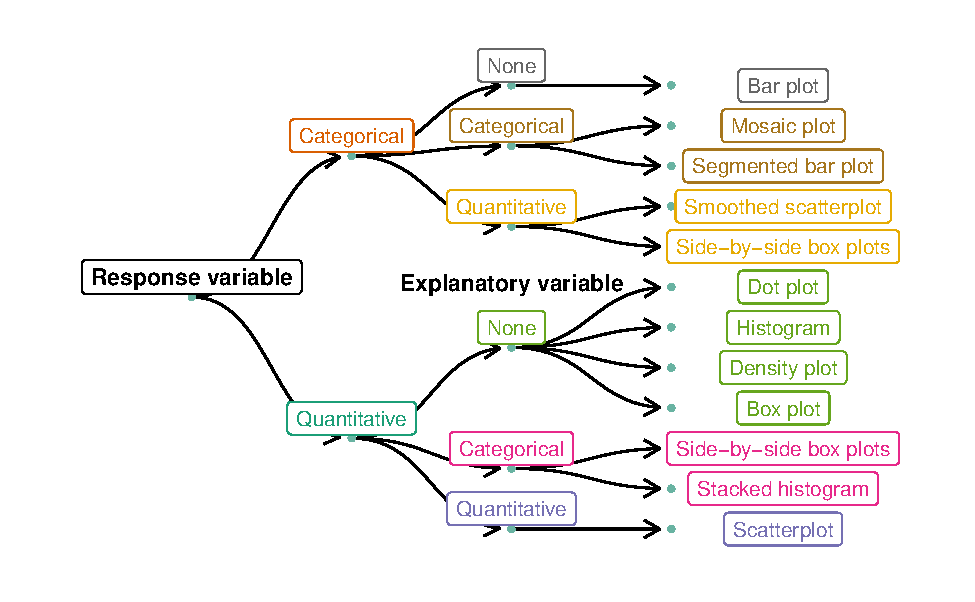
\includegraphics[width=0.7\linewidth]{04-RG-multivariate_files/figure-latex/decision-tree-plots-1} \end{center}

\hypertarget{section-7.1-gapminder-world}{%
\subsection*{Section 7.1 (Gapminder world)}\label{section-7.1-gapminder-world}}
\addcontentsline{toc}{subsection}{Section 7.1 (Gapminder world)}

\setstretch{1}

\textbf{Videos}

\begin{itemize}
\tightlist
\item
  Chapter7
\end{itemize}

\setstretch{1.25}

\hypertarget{vocabulary-8}{%
\subsubsection*{Vocabulary}\label{vocabulary-8}}
\addcontentsline{toc}{subsubsection}{Vocabulary}

Interaction:
\rgs

Aesthetic:
\rgs

\hypertarget{notes-11}{%
\subsubsection*{Notes}\label{notes-11}}
\addcontentsline{toc}{subsubsection}{Notes}

Use color and a legend to add a third variable to a scatterplot. E.g., Color the dots to represent different levels of a categorical variable or use shading of the dots to represent different values of a quantitative variable.

If the response and one predictor are quantitative and the other predictor is categorical, we fit a regression line for each level of the categorical predictor.

\begin{itemize}
\item
  Parallel slopes would indicate that that the two predictors \_\_\_\_\_\_\_\_\_\_\_\_\_\_\_\_\_\_\_ in explaining the response.
\item
  Non-parallel slopes would indicate that the two predictors \_\_\_\_\_\_\_\_\_\_\_\_\_\_\_\_\_\_\_ in explaining the response.
\end{itemize}

True or false: Scatterplots can only display two variables at a time.

\hypertarget{section-7.2-simpsons-paradox-revisited}{%
\subsection*{Section 7.2 (Simpson's Paradox, revisited)}\label{section-7.2-simpsons-paradox-revisited}}
\addcontentsline{toc}{subsection}{Section 7.2 (Simpson's Paradox, revisited)}

\setstretch{1}

\textbf{Videos}

\begin{itemize}
\tightlist
\item
  Chapter7
\end{itemize}

\setstretch{1.25}

\hypertarget{reminder-from-section-4.4}{%
\subsubsection*{Reminder from Section 4.4}\label{reminder-from-section-4.4}}
\addcontentsline{toc}{subsubsection}{Reminder from Section 4.4}

Simpson's Paradox: when the relationship between the explanatory and response variable is reversed when looking at the relationship within different levels of a confounding variable.

\hypertarget{notes-12}{%
\subsubsection*{Notes}\label{notes-12}}
\addcontentsline{toc}{subsubsection}{Notes}

True or false: Simpson's Paradox can only occur when the explanatory, response, and confounding variables are all categorical.

\hypertarget{example-sat-scores}{%
\subsubsection*{Example: SAT scores}\label{example-sat-scores}}
\addcontentsline{toc}{subsubsection}{Example: SAT scores}

\begin{enumerate}
\def\labelenumi{\arabic{enumi}.}
\item
  What are the observational units?\\
  \rgs
\item
  Look at the scatterplot in Figure 7.5.
\end{enumerate}

\rgi a) What is the explanatory variable? The response variable?
\rgs

\rgi b) What is the form of the scatterplot?
\rgs

\rgi c) What is the direction of the scatterplot?
\rgs

\rgi d) What is the strength of the scatterplot?
\rgs

\rgi e) Are there any outliers on the scatterplot?
\rgs

\begin{enumerate}
\def\labelenumi{\arabic{enumi}.}
\setcounter{enumi}{2}
\item
  What would need to be done to the study design in order to eliminate the confounding variable: percent of eligible students taking the SAT?
  \rgs
\item
  What features of the scatterplots in Figure 7.6 demonstrate that the percent of eligible students taking the SAT is a confounding variable?
  \rgs
\item
  How does Figure 7.7 demonstrate Simpson's Paradox?
  \rgs
\end{enumerate}

\newpage

\hypertarget{activity-4a-movie-profits-linear-regression}{%
\section{Activity 4A: Movie Profits --- Linear Regression}\label{activity-4a-movie-profits-linear-regression}}

\setstretch{1}

\hypertarget{learning-outcomes-8}{%
\subsection{Learning outcomes}\label{learning-outcomes-8}}

\begin{itemize}
\item
  Identify and create appropriate summary statistics and plots
  given a data set with two quantitative variables.
\item
  Use scatterplots to assess the relationship between two quantitative variables.
\item
  Find the estimated line of regression using summary statistics and R linear model (\texttt{lm()}) output.
\item
  Interpret the slope coefficient in context of the problem.
\end{itemize}

\hypertarget{terminology-review-8}{%
\subsection{Terminology review}\label{terminology-review-8}}

In today's activity, we will review summary measures and plots for two quantitative variables. Some terms covered in this activity are:

\begin{itemize}
\item
  Scatterplot
\item
  Least-squares line of regression
\item
  Slope and \(y\)-intercept
\item
  Residuals
\item
  Multivariable plots
\end{itemize}

To review these concepts, see Chapter 6 \& 7 in the textbook.

\hypertarget{movies-released-in-2016-1}{%
\subsection{Movies released in 2016}\label{movies-released-in-2016-1}}

A data set was collected on movies released in 2016 ({``{IMDb} Movies Extensive Dataset''} 2016). Here is a list of some of the variables collected on the observational units, movies released in 2016.

\begin{longtable}[]{@{}
  >{\raggedright\arraybackslash}p{(\columnwidth - 2\tabcolsep) * \real{0.2353}}
  >{\raggedright\arraybackslash}p{(\columnwidth - 2\tabcolsep) * \real{0.7647}}@{}}
\toprule()
\begin{minipage}[b]{\linewidth}\raggedright
\textbf{Variable}
\end{minipage} & \begin{minipage}[b]{\linewidth}\raggedright
\textbf{Description}
\end{minipage} \\
\midrule()
\endhead
\texttt{budget\_mil} & Amount of money (in US \$ millions) budgeted for the production of the movie \\
\texttt{revenue\_mil} & Amount of money (in US \$ millions) the movie made after release \\
\texttt{duration} & Length of the movie (in minutes) \\
\texttt{content\_rating} & Rating of the movie (\texttt{G}, \texttt{PG}, \texttt{PG-13}, R, \texttt{Not\ Rated}) \\
\texttt{imdb\_score} & IMDb user rating score from 1 to 10 \\
\texttt{genres} & Categories the movie falls into (e.g., Action, Drama, etc.) \\
\texttt{facebook\_likes} & Number of likes a movie receives on Facebook \\
\bottomrule()
\end{longtable}

\begin{Shaded}
\begin{Highlighting}[]
\NormalTok{movies }\OtherTok{\textless{}{-}} \FunctionTok{read.csv}\NormalTok{(}\StringTok{"https://math.montana.edu/courses/s216/data/Movies2016.csv"}\NormalTok{) }\CommentTok{\# Reads in data set }
\end{Highlighting}
\end{Shaded}

\hypertarget{vocabulary-review}{%
\subsubsection*{Vocabulary review}\label{vocabulary-review}}
\addcontentsline{toc}{subsubsection}{Vocabulary review}

To look at the relationship between two quantitative variables we will create a scatterplot with the explanatory variable on the x-axis and the response variable on the y-axis. We can also find three summary measures for the linear relationship between the two variables: regression slope, correlation and the coefficient of determination.

We will look at the relationship between budget and revenue for movies released in 2016. Upload and open the Movie Profits Activity 4A F22 Code R script file. Enter the explanatory variable name, \texttt{budget\_mil}, for \texttt{explanatory} and the response variable name, \texttt{revenue\_mil}, for \texttt{response} at line 7 in the R script file to create the scatterplot. (Note: both variables are measured in ``millions of dollars'' (\$MM).) Highlight and run lines 1--12.

\begin{Shaded}
\begin{Highlighting}[]
\NormalTok{movies }\SpecialCharTok{\%\textgreater{}\%} \CommentTok{\# Data set pipes into...}
\FunctionTok{ggplot}\NormalTok{(}\FunctionTok{aes}\NormalTok{(}\AttributeTok{x =}\NormalTok{ explanatory, }\AttributeTok{y =}\NormalTok{ response))}\SpecialCharTok{+}  \CommentTok{\# Specify variables}
  \FunctionTok{geom\_point}\NormalTok{() }\SpecialCharTok{+}  \CommentTok{\# Add scatterplot of points}
  \FunctionTok{labs}\NormalTok{(}\AttributeTok{x =} \StringTok{"Budget in Millions ($)"}\NormalTok{,  }\CommentTok{\# Label x{-}axis}
       \AttributeTok{y =} \StringTok{"Revenue in Millions ($)"}\NormalTok{,  }\CommentTok{\# Label y{-}axis}
       \AttributeTok{title =} \StringTok{"Revenue vs. Budget"}\NormalTok{) }\SpecialCharTok{+} \CommentTok{\# Be sure to title your plots}
  \FunctionTok{geom\_smooth}\NormalTok{(}\AttributeTok{method =} \StringTok{"lm"}\NormalTok{, }\AttributeTok{se =} \ConstantTok{FALSE}\NormalTok{)  }\CommentTok{\# Add regression line}
\end{Highlighting}
\end{Shaded}

\begin{enumerate}
\def\labelenumi{\arabic{enumi}.}
\tightlist
\item
  Sketch the scatterplot created from the code.
\end{enumerate}

\vspace{2in}

\begin{enumerate}
\def\labelenumi{\arabic{enumi}.}
\setcounter{enumi}{1}
\tightlist
\item
  Assess the four features of the scatterplot that describe this relationship. Describe each feature using a complete sentence!
\end{enumerate}

\begin{itemize}
\tightlist
\item
  Form (linear, non-linear)
\end{itemize}

\vspace{.2in}

\begin{itemize}
\tightlist
\item
  Direction (positive, negative)
\end{itemize}

\vspace{.2in}

\begin{itemize}
\tightlist
\item
  Strength
\end{itemize}

\vspace{.2in}

\begin{itemize}
\tightlist
\item
  Unusual observations or outliers
\end{itemize}

\vspace{.2in}

\begin{enumerate}
\def\labelenumi{\arabic{enumi}.}
\setcounter{enumi}{2}
\tightlist
\item
  Based on the plot, does there appear to be an association between budget and revenue? Explain.
\end{enumerate}

\vspace{1in}

\hypertarget{slope}{%
\subsubsection*{Slope}\label{slope}}
\addcontentsline{toc}{subsubsection}{Slope}

The linear model function in R (\texttt{lm()}) gives us the summary for the least squares regression line. The estimate for \texttt{(Intercept)} is the \(y\)-intercept for the line of least squares, and the estimate for \texttt{budget\_mil} (the \(x\)-variable name) is the value of \(b_1\), the slope. Run lines 16 -- 17 in the R script file to reproduce the linear model output found in the coursepack.

\begin{Shaded}
\begin{Highlighting}[]
\CommentTok{\# Fit linear model: y \textasciitilde{} x}
\NormalTok{revenueLM }\OtherTok{\textless{}{-}} \FunctionTok{lm}\NormalTok{(revenue\_mil }\SpecialCharTok{\textasciitilde{}}\NormalTok{ budget\_mil, }\AttributeTok{data=}\NormalTok{movies)}
\FunctionTok{summary}\NormalTok{(revenueLM)}\SpecialCharTok{$}\NormalTok{coefficients }\CommentTok{\# Display coefficient summary}
\end{Highlighting}
\end{Shaded}

\begin{verbatim}
#>              Estimate Std. Error  t value     Pr(>|t|)
#> (Intercept) 9.1693054  9.0175499 1.016829 3.119606e-01
#> budget_mil  0.9460001  0.1056786 8.951670 4.339561e-14
\end{verbatim}

\begin{enumerate}
\def\labelenumi{\arabic{enumi}.}
\setcounter{enumi}{3}
\tightlist
\item
  Write out the least squares regression line using the summary statistics provided above in context of the problem.
  \vspace{0.8in}
\end{enumerate}

You may remember from middle and high school that slope \(=\frac{\mbox{rise}}{\mbox{run}}\).

Using \(b_1\) to represent slope, we can write that as the fraction \(\frac{b_1}{1}\).

Therefore, the slope predicts how much the line will \emph{rise} for each \emph{run} of +1. In other words, as the \(x\) variable increases by 1 unit, the \(y\) variable is predicted to change (increase/decrease) by the value of slope.

\begin{enumerate}
\def\labelenumi{\arabic{enumi}.}
\setcounter{enumi}{4}
\tightlist
\item
  Interpret the value of slope in context of the problem.
\end{enumerate}

\vspace{.8in}

\begin{enumerate}
\def\labelenumi{\arabic{enumi}.}
\setcounter{enumi}{5}
\tightlist
\item
  Using the least squares line from question 4, predict the revenue for a movie with a budget of 165 \$MM.
\end{enumerate}

\vspace{.6in}

\begin{enumerate}
\def\labelenumi{\arabic{enumi}.}
\setcounter{enumi}{6}
\tightlist
\item
  Predict the revenue for a movie with a budget of 500 \$MM.
\end{enumerate}

\vspace{0.8in}

\begin{enumerate}
\def\labelenumi{\arabic{enumi}.}
\setcounter{enumi}{7}
\tightlist
\item
  The prediction in question 7 is an example of what?
\end{enumerate}

\vspace{0.3in}

\hypertarget{residuals}{%
\subsubsection*{Residuals}\label{residuals}}
\addcontentsline{toc}{subsubsection}{Residuals}

The model we are using assumes the relationship between the two variables follows a straight line. The residuals are the errors, or the variability in the response that hasn't been modeled by the line (model).

\begin{center}
Data = Model + Residual

$\implies$ Residual = Data $-$ Model

$e_i=y_i-\hat{y}_i$
\end{center}

\begin{enumerate}
\def\labelenumi{\arabic{enumi}.}
\setcounter{enumi}{8}
\tightlist
\item
  The movie \emph{Independence Day: Resurgence} had a budget of 165 \$MM and revenue of 102.315 \$MM. Find the residual for this movie.
\end{enumerate}

\vspace{.8in}

\begin{enumerate}
\def\labelenumi{\arabic{enumi}.}
\setcounter{enumi}{9}
\tightlist
\item
  Did the line of regression overestimate or underestimate the revenue for this movie?
\end{enumerate}

\vspace{.2in}

\hypertarget{multivariable-plots}{%
\subsubsection*{Multivariable plots}\label{multivariable-plots}}
\addcontentsline{toc}{subsubsection}{Multivariable plots}

What if we wanted to see if the relationship between movie budget and revenue differs if we add another variable into the picture? The following plot visualizes three variables, creating a \textbf{multivariable} plot.

\begin{Shaded}
\begin{Highlighting}[]
\NormalTok{movies }\SpecialCharTok{\%\textgreater{}\%} \CommentTok{\# Data set pipes into...}
  \FunctionTok{filter}\NormalTok{(content\_rating }\SpecialCharTok{!=} \StringTok{"Not Rated"}\NormalTok{) }\SpecialCharTok{\%\textgreater{}\%} \CommentTok{\# Remove Not Rated movies}
  \FunctionTok{ggplot}\NormalTok{(}\FunctionTok{aes}\NormalTok{(}\AttributeTok{x =}\NormalTok{ budget\_mil, }\AttributeTok{y =}\NormalTok{ revenue\_mil, }\AttributeTok{color =}\NormalTok{ content\_rating)) }\SpecialCharTok{+}  \CommentTok{\# Specify variables}
  \FunctionTok{geom\_point}\NormalTok{(}\FunctionTok{aes}\NormalTok{(}\AttributeTok{shape =}\NormalTok{ content\_rating), }\AttributeTok{size =} \DecValTok{3}\NormalTok{) }\SpecialCharTok{+}  \CommentTok{\# Add scatterplot of points}
  \FunctionTok{labs}\NormalTok{(}\AttributeTok{x =} \StringTok{"Budget in Millions ($)"}\NormalTok{,  }\CommentTok{\# Label x{-}axis}
       \AttributeTok{y =} \StringTok{"Revenue in Millions ($)"}\NormalTok{,  }\CommentTok{\# Label y{-}axis}
       \AttributeTok{color =} \StringTok{"content\_rating"}\NormalTok{,  }\CommentTok{\# Label legend}
       \AttributeTok{title =} \StringTok{"Revenue vs. Budget"}\NormalTok{) }\SpecialCharTok{+} \CommentTok{\# Be sure to tile your plots}
  \FunctionTok{geom\_smooth}\NormalTok{(}\AttributeTok{method =} \StringTok{"lm"}\NormalTok{, }\AttributeTok{se =} \ConstantTok{FALSE}\NormalTok{, }\AttributeTok{lwd =} \DecValTok{2}\NormalTok{) }\SpecialCharTok{+} \CommentTok{\# Add regression lines}
  \FunctionTok{scale\_color\_grey}\NormalTok{() }\CommentTok{\# Make black and white}
\end{Highlighting}
\end{Shaded}

\begin{center}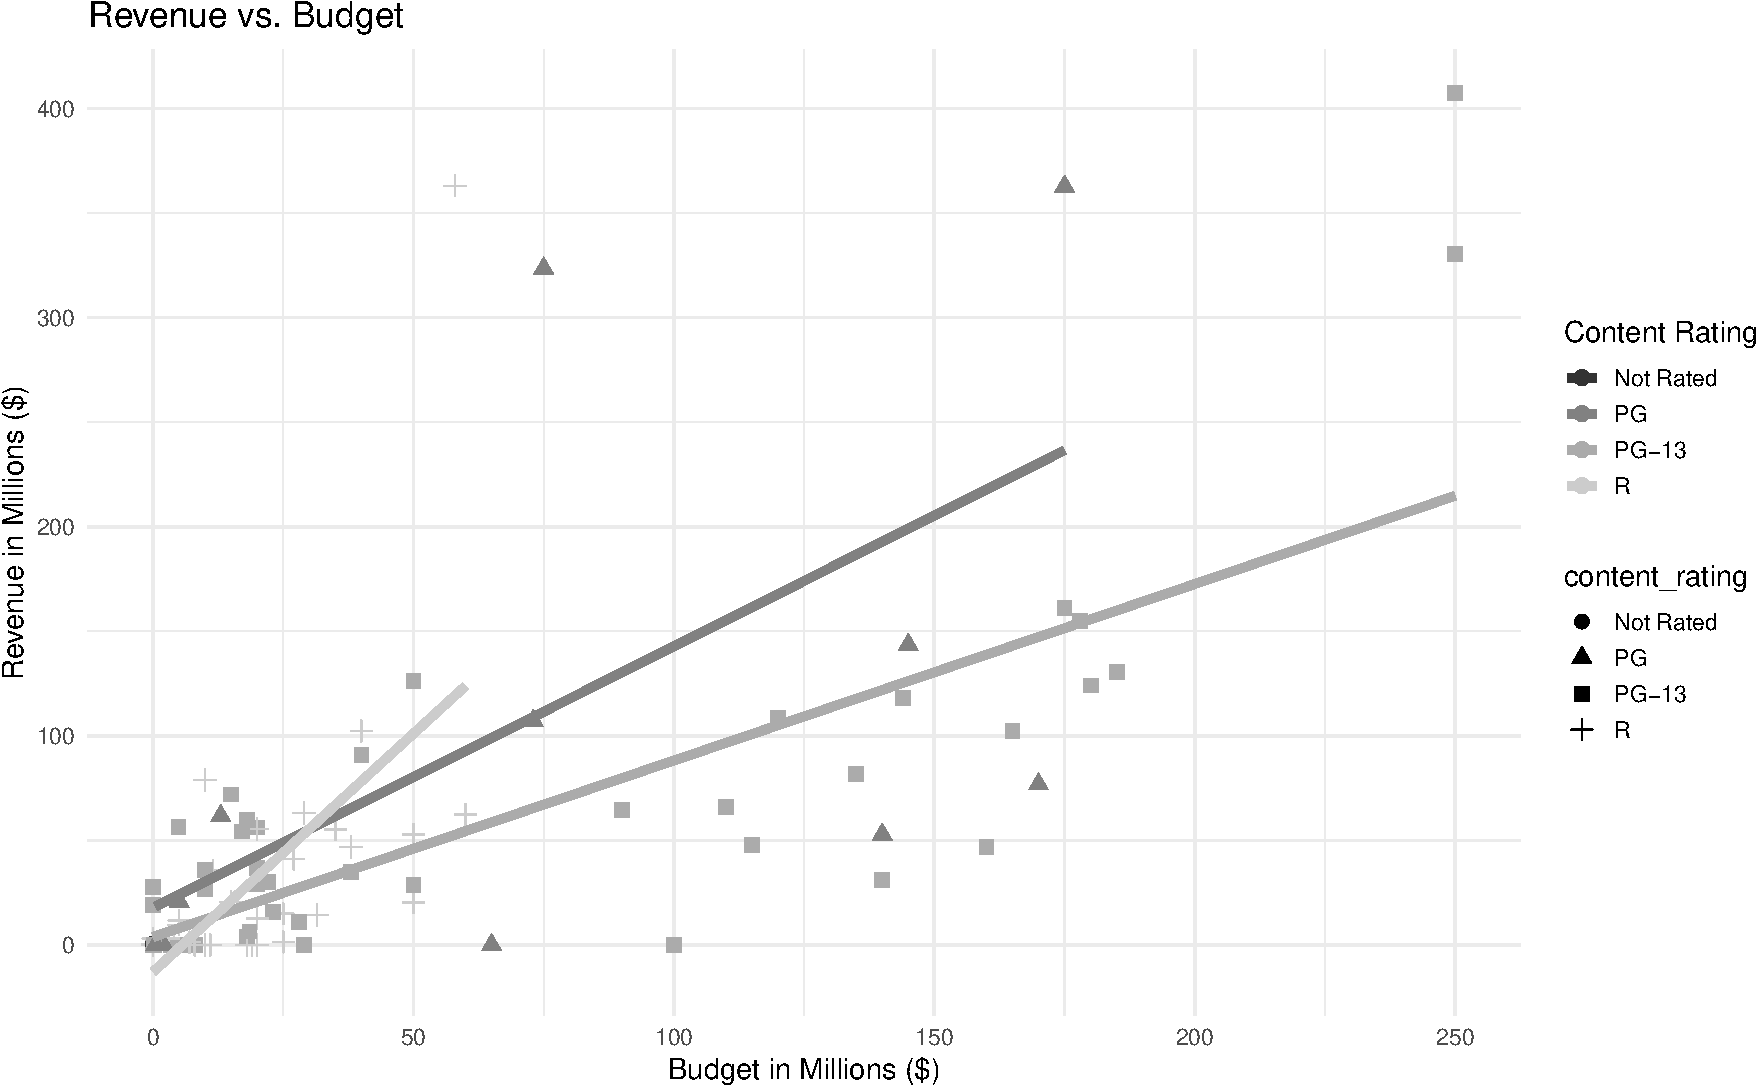
\includegraphics[width=0.7\linewidth]{04-A05-EDA-two-quantitative-PartA_files/figure-latex/unnamed-chunk-4-1} \end{center}

\begin{enumerate}
\def\labelenumi{\arabic{enumi}.}
\setcounter{enumi}{10}
\tightlist
\item
  Identify the three variables plotted in this graph.
\end{enumerate}

\vspace{0.5in}

\begin{enumerate}
\def\labelenumi{\arabic{enumi}.}
\setcounter{enumi}{11}
\tightlist
\item
  Does the \emph{relationship} between movie budget and revenue differ among the different content ratings? Explain.
\end{enumerate}

\vspace{0.8in}
\newpage

\hypertarget{take-home-messages-7}{%
\subsection{Take-home messages}\label{take-home-messages-7}}

\begin{enumerate}
\def\labelenumi{\arabic{enumi}.}
\item
  Two quantitative variables are graphically displayed in a scatterplot. The explanatory variable is on the \(x\)-axis and the response variable is on the \(y\)-axis. When describing the relationship between two quantitative variables we look at the form (linear or non-linear), direction (positive or negative), strength, and for the presence of outliers.
\item
  There are three summary statistics used to summarize the relationship between two quantitative variables: correlation (\(R\)), slope of the regression line (\(b_1\)), and the coefficient of determination (\(R^2\)).
\item
  We can use the line of regression to predict values of the response variable for values of the explanatory variable. Do not use values of the explanatory variable that are outside of the range of values in the data set to predict values of the response variable (reflect on why this is true.). This is called \textbf{extrapolation}.
\end{enumerate}

\hypertarget{additional-notes-7}{%
\subsection{Additional notes}\label{additional-notes-7}}

Use this space to summarize your thoughts and take additional notes on today's activity and material covered.

\newpage

\hypertarget{activity-4b-movie-profits-correlation-and-coefficient-of-determination}{%
\section{Activity 4B: Movie Profits --- Correlation and Coefficient of Determination}\label{activity-4b-movie-profits-correlation-and-coefficient-of-determination}}

\setstretch{1}

\hypertarget{learning-outcomes-9}{%
\subsection{Learning outcomes}\label{learning-outcomes-9}}

\begin{itemize}
\item
  Identify and create appropriate summary statistics and plots
  given a data set with two quantitative variables.
\item
  Calculate and interpret \(r^2\), the coefficient of determination, in context of the problem.
\item
  Find the correlation coefficient from R output or from \(r^2\) and the sign of the slope.
\end{itemize}

\hypertarget{terminology-review-9}{%
\subsection{Terminology review}\label{terminology-review-9}}

In today's activity, we will review summary measures and plots for two quantitative variables. Some terms covered in this activity are:

\begin{itemize}
\item
  Correlation (\(r\))
\item
  Coefficient of determination (\(r\)-squared or \(r^2\))
\end{itemize}

To review these concepts, see Chapter 6 in the textbook.

\hypertarget{movies-released-in-2016-2}{%
\subsection{Movies released in 2016}\label{movies-released-in-2016-2}}

We will revisit the movie data set collected on Movies released in 2016 ({``{IMDb} Movies Extensive Dataset''} 2016) to further explore the relationship between budget and revenue. Here is a reminder of the variables collected on these movies.

\begin{longtable}[]{@{}
  >{\raggedright\arraybackslash}p{(\columnwidth - 2\tabcolsep) * \real{0.2353}}
  >{\raggedright\arraybackslash}p{(\columnwidth - 2\tabcolsep) * \real{0.7647}}@{}}
\toprule()
\begin{minipage}[b]{\linewidth}\raggedright
\textbf{Variable}
\end{minipage} & \begin{minipage}[b]{\linewidth}\raggedright
\textbf{Description}
\end{minipage} \\
\midrule()
\endhead
\texttt{budget\_mil} & Amount of money (in US \$ millions) budgeted for the production of the movie \\
\texttt{revenue\_mil} & Amount of money (in US \$ millions) the movie made after release \\
\texttt{duration} & Length of the movie (in minutes) \\
\texttt{content\_rating} & Rating of the movie (\texttt{G}, \texttt{PG}, \texttt{PG-13}, R, \texttt{Not\ Rated}) \\
\texttt{imdb\_score} & IMDb user rating score from 1 to 10 \\
\texttt{genres} & Categories the movie falls into (e.g., Action, Drama, etc.) \\
\texttt{facebook\_likes} & Number of likes a movie receives on Facebook \\
\bottomrule()
\end{longtable}

\newpage

\hypertarget{correlation}{%
\subsubsection*{Correlation}\label{correlation}}
\addcontentsline{toc}{subsubsection}{Correlation}

Correlation measures the strength and the direction of the linear relationship between two quantitative variables. The closer the value of correlation to \(+1\) or \(-1\), the stronger the linear relationship. Values close to zero indicate a very weak linear relationship between the two variables. The following output shows a correlation matrix between several pairs of quantitative variables. Upload and open the Movie Profits Activity 4B F22 Code R script file. Highlight and run lines 1--12 to produce the same table as below.

\begin{Shaded}
\begin{Highlighting}[]
\NormalTok{movies }\OtherTok{\textless{}{-}} \FunctionTok{read.csv}\NormalTok{(}\StringTok{"https://math.montana.edu/courses/s216/data/Movies2016.csv"}\NormalTok{) }\CommentTok{\# Reads in data set}
\NormalTok{movies }\SpecialCharTok{\%\textgreater{}\%}  \CommentTok{\# Data set pipes into}
  \FunctionTok{select}\NormalTok{(}\FunctionTok{c}\NormalTok{(}\StringTok{"budget\_mil"}\NormalTok{, }\StringTok{"revenue\_mil"}\NormalTok{, }
           \StringTok{"duration"}\NormalTok{, }\StringTok{"imdb\_score"}\NormalTok{, }
           \StringTok{"facebook\_likes"}\NormalTok{)) }\SpecialCharTok{\%\textgreater{}\%}
  \FunctionTok{cor}\NormalTok{(}\AttributeTok{use=}\StringTok{"pairwise.complete.obs"}\NormalTok{) }\SpecialCharTok{\%\textgreater{}\%}
  \FunctionTok{round}\NormalTok{(}\DecValTok{3}\NormalTok{)}
\end{Highlighting}
\end{Shaded}

\begin{verbatim}
#>                budget_mil revenue_mil duration imdb_score facebook_likes
#> budget_mil          1.000       0.686    0.463      0.292          0.678
#> revenue_mil         0.686       1.000    0.227      0.398          0.723
#> duration            0.463       0.227    1.000      0.261          0.438
#> imdb_score          0.292       0.398    0.261      1.000          0.309
#> facebook_likes      0.678       0.723    0.438      0.309          1.000
\end{verbatim}

\begin{enumerate}
\def\labelenumi{\arabic{enumi}.}
\tightlist
\item
  Using the output above, which two variables have the \emph{strongest} correlation? What is the value of this correlation?
\end{enumerate}

\vspace{0.5in}

\begin{enumerate}
\def\labelenumi{\arabic{enumi}.}
\setcounter{enumi}{1}
\tightlist
\item
  What is the value of correlation between budget and revenue?
\end{enumerate}

\vspace{0.3in}

\begin{enumerate}
\def\labelenumi{\arabic{enumi}.}
\setcounter{enumi}{2}
\tightlist
\item
  Based on the value of correlation found in question 2, what would the sign of the slope be? Positive or negative? Explain.
\end{enumerate}

\vspace{0.5in}

\begin{enumerate}
\def\labelenumi{\arabic{enumi}.}
\setcounter{enumi}{3}
\tightlist
\item
  Does your answer to question 3 match the direction you choose in question 2 in Activity 4A?
\end{enumerate}

\vspace{0.3in}

\begin{enumerate}
\def\labelenumi{\arabic{enumi}.}
\setcounter{enumi}{4}
\tightlist
\item
  Explain why the correlation values on the diagonal are equal to 1.
\end{enumerate}

\vspace{0.8in}
\newpage

\hypertarget{coefficient-of-determination-squared-correlation}{%
\subsubsection*{Coefficient of determination (squared correlation)}\label{coefficient-of-determination-squared-correlation}}
\addcontentsline{toc}{subsubsection}{Coefficient of determination (squared correlation)}

Another summary measure used to explain the linear relationship between two quantitative variables is the coefficient of determination (\(r^2\)). The coefficient of determination, \(r^2\), can also be used to describe the strength of the linear relationship between two quantitative variables. The value of \(R^2\) (a value between 0 and 1) represents the \textbf{proportion of variation in the response that is explained by the least squares line with the explanatory variable}. There are two ways to calculate the coefficient of determination:

~~~Square the correlation coefficient: \(r^2 = (r)^2\)

~~~Use the variances of the response and the residuals: \(r^2 = \dfrac{s_y^2 - s_{RES}^2}{s_y^2} = \dfrac{SST - SSE}{SST}\)

\begin{enumerate}
\def\labelenumi{\arabic{enumi}.}
\setcounter{enumi}{5}
\tightlist
\item
  Use the correlation, \(r\), found in question 2 of the activity, to calculate the coefficient of determination between budget and revenue, \(r^2\).
\end{enumerate}

\vspace{.4in}

\begin{enumerate}
\def\labelenumi{\arabic{enumi}.}
\setcounter{enumi}{6}
\tightlist
\item
  The variance of the response variable, revenue in \$MM, is about \(s_{revenue}^2 = 8024.261\) \$MM\(^2\) and the variability in the residuals is about \(s_{RES}^2 = 4244.832\) \$MM\(^2\). Use these values to calculate the coefficient of determination. Verify that your answers to 6 and 7 are the same.
\end{enumerate}

\vspace{1in}

In the next part of the activity we will explore what the coefficient of determination measures.

\begin{itemize}
\item
  Go to the website www.rossmanchance.com/ISIapplets.html and click on Corr/Regresssion under Quantitative Response.
\item
  Click \texttt{Clear} below the box containing the sample data.
\item
  Download and open the csv file ``Movie2016'' from D2L. Copy the two columns containing \texttt{budget\_mil} and \texttt{revenue\_mil} including the headers and paste into the sample data box.
\item
  Click 'Use Data`.
\end{itemize}

\begin{enumerate}
\def\labelenumi{\arabic{enumi}.}
\setcounter{enumi}{7}
\tightlist
\item
  Click on \texttt{Show\ Moveable\ Line}. Write down the equation of the line given. Why is the slope zero for this line?
\end{enumerate}

\vspace{0.8in}

\begin{enumerate}
\def\labelenumi{\arabic{enumi}.}
\setcounter{enumi}{8}
\tightlist
\item
  Click on \texttt{Show\ Squared\ Residuals}. Write down the value for SSE. Since this is the sum of squared errors (SSE) for the horizontal line we call this the total sum of squares (SST).
\end{enumerate}

\newpage

\begin{enumerate}
\def\labelenumi{\arabic{enumi}.}
\setcounter{enumi}{9}
\tightlist
\item
  Click on \texttt{Show\ Regression\ Line}. Write down the equation of the line given. Does this match the least squares line found in Activity 4A question 4?
\end{enumerate}

\vspace{1in}

\begin{enumerate}
\def\labelenumi{\arabic{enumi}.}
\setcounter{enumi}{10}
\tightlist
\item
  Click on \texttt{Show\ Squared\ Residuals}. Write down the value for SSE.
\end{enumerate}

\vspace{0.5in}

\begin{enumerate}
\def\labelenumi{\arabic{enumi}.}
\setcounter{enumi}{11}
\tightlist
\item
  Calculate the value for \(r^2\) using the values found for SST and SSE.
\end{enumerate}

\vspace{1in}

\begin{enumerate}
\def\labelenumi{\arabic{enumi}.}
\setcounter{enumi}{12}
\tightlist
\item
  Write a sentence interpreting the coefficient of determination in context of the problem.
\end{enumerate}

\newpage

\hypertarget{take-home-messages-8}{%
\subsection{Take-home messages}\label{take-home-messages-8}}

\begin{enumerate}
\def\labelenumi{\arabic{enumi}.}
\item
  The sign of correlation and the sign of the slope will always be the same. The closer the value of correlation is to \(-1\) or \(+1\), the stronger the relationship between the explanatory and the response variable.
\item
  The coefficient of determination multiplied by 100 (\(r^2 \times 100\)) measures the percent of variation in the response variable that is explained by the relationship with the explanatory variable. The closer the value of the coefficient of determination is to 100\%, the stronger the relationship.
\end{enumerate}

\hypertarget{additional-notes-8}{%
\subsection{Additional notes}\label{additional-notes-8}}

Use this space to summarize your thoughts and take additional notes on today's activity and material covered.

\newpage

\hypertarget{week-4-lab-penguins}{%
\section{Week 4 Lab: Penguins}\label{week-4-lab-penguins}}

\setstretch{1}

\hypertarget{learning-outcomes-10}{%
\subsection{Learning outcomes}\label{learning-outcomes-10}}

\begin{itemize}
\item
  Identify and create appropriate summary statistics and plots
  given a data set with two quantitative variables.
\item
  Use scatterplots to assess the relationship between two quantitative variables.
\item
  Find the estimated line of regression using summary statistics and R linear model (\texttt{lm()}) output.
\item
  Interpret the slope coefficient in context of the problem.
\item
  Calculate and interpret \(R^2\), the coefficient of determination, in context of the problem.
\item
  Find the correlation coefficient from R output or from \(R^2\) and the sign of the slope.
\end{itemize}

\hypertarget{penguins}{%
\subsection{Penguins}\label{penguins}}

The Palmer Station Long Term Ecological Research Program sampled three penguin species on islands in the Palmer Archipelago in Antarctica. Researchers took various body measurements on the penguins, including flipper length and body mass. The researchers were interested in the relationship between flipper length and body mass and wondered if flipper length could be used to accurately predict the body mass of these three penguin species.

Upload and import the \texttt{Antarctica\_Penguins} csv file and the provided R script file for week 4 lab. Enter the name of the data set (see the environment tab) for \texttt{datasetname} in the R script file in line 4.

First we will create a scatterplot of the flipper length and body mass. Notice that we are using flipper length to predict body mass. This makes flipper length the explanatory variable. \textbf{Make sure to give your plot a descriptive title.} Highlight and run lines 1--13 in the R script file. \textbf{Upload a copy of your scatterplot to Gradescope.}

\begin{Shaded}
\begin{Highlighting}[]
\NormalTok{penguins }\OtherTok{\textless{}{-}}\NormalTok{ datasetname }\CommentTok{\#Creates the object penguins}
\NormalTok{penguins }\SpecialCharTok{\%\textgreater{}\%}
  \FunctionTok{ggplot}\NormalTok{(}\FunctionTok{aes}\NormalTok{(}\AttributeTok{x =}\NormalTok{ flipper\_length\_mm, }\AttributeTok{y =}\NormalTok{ body\_mass\_g))}\SpecialCharTok{+}  \CommentTok{\# Specify variables}
  \FunctionTok{geom\_point}\NormalTok{() }\SpecialCharTok{+}  \CommentTok{\# Add scatterplot of points}
  \FunctionTok{labs}\NormalTok{(}\AttributeTok{x =} \StringTok{"flipper length (mm)"}\NormalTok{,  }\CommentTok{\# Label x{-}axis}
       \AttributeTok{y =} \StringTok{"body mass (g)"}\NormalTok{,  }\CommentTok{\# Label y{-}axis}
       \AttributeTok{title =} \StringTok{"Title"}\NormalTok{) }\SpecialCharTok{+} \CommentTok{\# Be sure to title your plots}
  \FunctionTok{geom\_smooth}\NormalTok{(}\AttributeTok{method =} \StringTok{"lm"}\NormalTok{, }\AttributeTok{se =} \ConstantTok{FALSE}\NormalTok{)  }\CommentTok{\# Add regression line}
\end{Highlighting}
\end{Shaded}

\begin{enumerate}
\def\labelenumi{\arabic{enumi}.}
\tightlist
\item
  Assess the four features of the scatterplot that describe this relationship.
  \vspace{1mm}
\end{enumerate}

\begin{itemize}
\tightlist
\item
  Form (linear, non-linear)
\end{itemize}

\vspace{.1in}

\begin{itemize}
\tightlist
\item
  Direction (positive, negative)
\end{itemize}

\vspace{.1in}

\begin{itemize}
\tightlist
\item
  Strength
\end{itemize}

\vspace{.1in}

\begin{itemize}
\tightlist
\item
  Unusual observations or outliers
\end{itemize}

\vspace{.1in}

Highlight and run lines 16--20 to get the correlation matrix in the R script file.

\begin{Shaded}
\begin{Highlighting}[]
\NormalTok{penguins }\SpecialCharTok{\%\textgreater{}\%}  \CommentTok{\# Data set pipes into}
  \FunctionTok{select}\NormalTok{(}\FunctionTok{c}\NormalTok{(}\StringTok{"bill\_length\_mm"}\NormalTok{, }\StringTok{"bill\_depth\_mm"}\NormalTok{, }
           \StringTok{"flipper\_length\_mm"}\NormalTok{, }\StringTok{"body\_mass\_g"}\NormalTok{)) }\SpecialCharTok{\%\textgreater{}\%}
  \FunctionTok{cor}\NormalTok{(}\AttributeTok{use=}\StringTok{"pairwise.complete.obs"}\NormalTok{) }\SpecialCharTok{\%\textgreater{}\%}
  \FunctionTok{round}\NormalTok{(}\DecValTok{3}\NormalTok{)}
\end{Highlighting}
\end{Shaded}

\begin{enumerate}
\def\labelenumi{\arabic{enumi}.}
\setcounter{enumi}{1}
\tightlist
\item
  Using the R output, which two variables have the \emph{strongest} correlation? What is the value of this correlation?
\end{enumerate}

\vspace{0.5in}

\begin{enumerate}
\def\labelenumi{\arabic{enumi}.}
\setcounter{enumi}{2}
\tightlist
\item
  Using the value of correlation found in question 2, calculate the value of the coefficient of determination.
\end{enumerate}

\vspace{0.5in}

\begin{enumerate}
\def\labelenumi{\arabic{enumi}.}
\setcounter{enumi}{3}
\tightlist
\item
  \textbf{Interpret the coefficient of determination in context of the problem.}
\end{enumerate}

\vspace{1in}

Enter the variable \texttt{body\_mass\_g} for \texttt{response} and the variable name \texttt{flipper\_length\_mm} for \texttt{explanatory} in line 23 in the R script file. Highlight and run lines 23--24 to get the linear model output.

\begin{Shaded}
\begin{Highlighting}[]
\CommentTok{\# Fit linear model: y \textasciitilde{} x}
\NormalTok{penguinsLM }\OtherTok{\textless{}{-}} \FunctionTok{lm}\NormalTok{(response}\SpecialCharTok{\textasciitilde{}}\NormalTok{explanatory, }\AttributeTok{data=}\NormalTok{penguins)}
\FunctionTok{summary}\NormalTok{(penguinsLM)}\SpecialCharTok{$}\NormalTok{coefficients }\CommentTok{\# Display coefficient summary}
\end{Highlighting}
\end{Shaded}

\begin{enumerate}
\def\labelenumi{\arabic{enumi}.}
\setcounter{enumi}{4}
\tightlist
\item
  Write out the least squares regression line using the summary statistics from the R output in context of the problem.
\end{enumerate}

\vspace{.5in}

\begin{enumerate}
\def\labelenumi{\arabic{enumi}.}
\setcounter{enumi}{5}
\tightlist
\item
  \textbf{Interpret the value of slope in context of the problem.}
\end{enumerate}

\vspace{.8in}

\begin{enumerate}
\def\labelenumi{\arabic{enumi}.}
\setcounter{enumi}{6}
\tightlist
\item
  \textbf{Using the least squares regression line from question 5, predict the body mass for a penguin with a flipper length of 181 mm.}
\end{enumerate}

\vspace{.6in}

\begin{enumerate}
\def\labelenumi{\arabic{enumi}.}
\setcounter{enumi}{7}
\tightlist
\item
  One penguin had a flipper length of 181 mm and a body mass of 3750 g. Find the residual for this penguin.
\end{enumerate}

\vspace{.8in}

\begin{enumerate}
\def\labelenumi{\arabic{enumi}.}
\setcounter{enumi}{8}
\tightlist
\item
  Did the line of regression overestimate or underestimate the body mass for this penguin?
\end{enumerate}

\vspace{0.5in}

Highlight and run lines 27--34 to get the multivariate plot.

\begin{Shaded}
\begin{Highlighting}[]
\NormalTok{penguins }\SpecialCharTok{\%\textgreater{}\%}
  \FunctionTok{ggplot}\NormalTok{(}\FunctionTok{aes}\NormalTok{(}\AttributeTok{x =}\NormalTok{ flipper\_length\_mm, }\AttributeTok{y =}\NormalTok{ body\_mass\_g, }\AttributeTok{color=}\NormalTok{species))}\SpecialCharTok{+}  \CommentTok{\# Specify variables}
  \FunctionTok{geom\_point}\NormalTok{(}\FunctionTok{aes}\NormalTok{(}\AttributeTok{shape =}\NormalTok{ species), }\AttributeTok{size =} \DecValTok{3}\NormalTok{) }\SpecialCharTok{+}  \CommentTok{\# Add scatterplot of points}
  \FunctionTok{labs}\NormalTok{(}\AttributeTok{x =} \StringTok{"flipper length (mm)"}\NormalTok{,  }\CommentTok{\# Label x{-}axis}
       \AttributeTok{y =} \StringTok{"body mass (g)"}\NormalTok{,  }\CommentTok{\# Label y{-}axis}
       \AttributeTok{color =} \StringTok{"species"}\NormalTok{,}
       \AttributeTok{title =} \StringTok{"TITLE"}\NormalTok{) }\SpecialCharTok{+} \CommentTok{\# Be sure to tile your plots}
  \FunctionTok{geom\_smooth}\NormalTok{(}\AttributeTok{method =} \StringTok{"lm"}\NormalTok{, }\AttributeTok{se =} \ConstantTok{FALSE}\NormalTok{)  }\CommentTok{\# Add regression line}
\end{Highlighting}
\end{Shaded}

\begin{enumerate}
\def\labelenumi{\arabic{enumi}.}
\setcounter{enumi}{9}
\tightlist
\item
  What three variables are plotted on this plot?
\end{enumerate}

\vspace{0.3in}

\begin{enumerate}
\def\labelenumi{\arabic{enumi}.}
\setcounter{enumi}{10}
\tightlist
\item
  \textbf{Does adding the variable species affect the relationship between body mass and flipper length? Explain your answer.}
\end{enumerate}

\vspace{0.5in}

\begin{enumerate}
\def\labelenumi{\arabic{enumi}.}
\setcounter{enumi}{11}
\tightlist
\item
  Explain the association between species and each of the other two variables.
\end{enumerate}

\newpage

\hypertarget{group-exam-1-review}{%
\chapter{Group Exam 1 Review}\label{group-exam-1-review}}

Use the provided data set from the Islands (ExamReviewData.csv) and the appropriate Exam 1 Review R script file to answer the following questions. Each adult (\textgreater21) islander was selected at random from all adult islanders. Variables and their descriptions are listed below. Music type (classical or heavy metal) was randomly assigned to the Islanders. Time to complete the puzzle cube was measured after listening to music for each Islander. Heart rate and blood glucose levels were both measured before and then after drinking a caffeinated beverage.

\begin{longtable}[]{@{}
  >{\raggedright\arraybackslash}p{(\columnwidth - 2\tabcolsep) * \real{0.2353}}
  >{\raggedright\arraybackslash}p{(\columnwidth - 2\tabcolsep) * \real{0.7647}}@{}}
\toprule()
\begin{minipage}[b]{\linewidth}\raggedright
\textbf{Variable}
\end{minipage} & \begin{minipage}[b]{\linewidth}\raggedright
\textbf{Description}
\end{minipage} \\
\midrule()
\endhead
\texttt{Island} & Name of Island that the Islander resides on \\
\texttt{City} & Name of City in which the Islander resides \\
\texttt{Population} & Population of the City \\
\texttt{Name} & Name of Islander \\
\texttt{Consent} & Whether the Islander consented to be in the study \\
\texttt{Gender} & Gender of Islander (M = male, F = Female) \\
\texttt{Age} & Age of Islander \\
\texttt{Married} & Marital status of Islander \\
\texttt{Smoking\_Status} & Whether the Islander is a current smoker \\
\texttt{Children} & Whether the Islander has children \\
\texttt{weight\_kg} & Weight measured in kg \\
\texttt{height\_cm} & Height measured in cm \\
\texttt{respiratory\_rate} & Breaths per minute \\
\texttt{Type\_of\_Music} & Music type (Classical or Heavy Medal) Islander was randomly assigned to listen to \\
\texttt{After\_PuzzleCube} & Time to complete puzzle cube (minutes) after listening to assigned music \\
\texttt{Education\_Level} & Highest level of education completed \\
\texttt{Balance\_Test} & Time balanced measured in seconds with eyes closed \\
\texttt{Blood\_Glucose\_before} & Level of blood glucose (mg/dL) before consuming assigned drink \\
\texttt{Heart\_Rate\_before} & Heart rate (bpm) before consuming assigned drink \\
\texttt{Blood\_Glucose\_after} & Level of blood glucose (mg/dL) after consuming assigned drink \\
\texttt{Heart\_Rate\_after} & Heart rate (bpm) after consuming assigned drink \\
\texttt{Diff\_Heart\_Rate} & Difference in heart rate (bpm) for Before - After consuming assigned drink \\
\texttt{Diff\_Blood\_Glucose} & Difference in blood glucose (mg/dL) for Before - After consuming assigned drink \\
\bottomrule()
\end{longtable}

\begin{enumerate}
\def\labelenumi{\arabic{enumi}.}
\tightlist
\item
  What are the observational units?
\end{enumerate}

\vspace{0.1in}

\begin{enumerate}
\def\labelenumi{\arabic{enumi}.}
\setcounter{enumi}{1}
\tightlist
\item
  In the table above, indicate which variables are categorical (C) and which variables are quantitative (Q).
\end{enumerate}

\vspace{0.1in}

\begin{enumerate}
\def\labelenumi{\arabic{enumi}.}
\setcounter{enumi}{2}
\tightlist
\item
  What type of bias may be present in this study? Explain.
\end{enumerate}

\vspace{0.5in}

\begin{enumerate}
\def\labelenumi{\arabic{enumi}.}
\setcounter{enumi}{3}
\tightlist
\item
  Use the appropriate Exam 1 Review R script file to find the appropriate summary statistic and graphical display of the data to assess the following research question, ``Is there a difference in proportion of Islanders who have children for those who completed high school and those that completed university?'' Use high school \(-\) university as the order of subtraction.
\end{enumerate}

\begin{enumerate}
\def\labelenumi{\alph{enumi}.}
\item
  What is the name of the explanatory variable to be assessed in this research question?
  \vspace{0.3in}

  What type of variable (categorical or quantitative) is the variable you identified?
  \vspace{0.3in}
\item
  What is the name of the response variable to be assessed in this research question?
  \vspace{0.3in}

  What type of variable (categorical or quantitative) is the variable you identified?
  \vspace{0.3in}
\item
  Use the R script file to get the counts for each level and combination of variables. Fill in the following table with the variable names, levels of each variable, and counts using the values from the R output.
\end{enumerate}

\begingroup
\setlength{\tabcolsep}{14pt}
\renewcommand{\arraystretch}{2}
\begin{center}
\begin{tabular}{|c|p{1in}|p{1in}|p{1in}|}
\hline
 & \multicolumn{2}{|c|}{\textbf{Explanatory Variable}} & \\ 
 & \multicolumn{2}{|c|}{ } & \\ \hline
\textbf{Response variable} & Group 1 & Group 2 & Total \\
 & & & \\ \hline
 Success & & & \\
 & & & \\ \hline
 Failure & & & \\
 & & & \\ \hline
 Total & & & \\
 & & & \\ \hline
\end{tabular}
\end{center}
\endgroup

\begin{enumerate}
\def\labelenumi{\alph{enumi}.}
\setcounter{enumi}{3}
\tightlist
\item
  Calculate the value of summary statistic to answer the research question. Give appropriate notation.
\end{enumerate}

\newpage

\begin{enumerate}
\def\labelenumi{\alph{enumi}.}
\setcounter{enumi}{4}
\item
  Interpret the value of the summary statistic in context of the problem:
  \vspace{0.5in}
\item
  What type of graph(s) would be appropriate for this research question?
\end{enumerate}

\vspace{0.2in}

\begin{enumerate}
\def\labelenumi{\alph{enumi}.}
\setcounter{enumi}{6}
\tightlist
\item
  Using the provided R file create a graph of the data. Sketch the graph below:
\end{enumerate}

\vspace{2in}

\begin{enumerate}
\def\labelenumi{\alph{enumi}.}
\setcounter{enumi}{7}
\tightlist
\item
  Based on the graph, does there appear to be an association between the two variables? Explain your answer.
\end{enumerate}

\vspace{0.5in}

\begin{enumerate}
\def\labelenumi{\roman{enumi}.}
\tightlist
\item
  Is this an observational study or a randomized experiment? Explain your answer.
\end{enumerate}

\vspace{0.5in}

\begin{enumerate}
\def\labelenumi{\alph{enumi}.}
\setcounter{enumi}{9}
\tightlist
\item
  What is the scope of inference for this study?
\end{enumerate}

\newpage

\begin{enumerate}
\def\labelenumi{\arabic{enumi}.}
\setcounter{enumi}{4}
\tightlist
\item
  Use the appropriate Exam 1 Review R script file to find the appropriate summary statistic and graphical display of the data to assess the following research question: ``Do Islanders who listen to classical music take less time to complete the puzzle cube after listening to the music than for Islanders that listen to heavy metal music?'' Use classical \(-\) heavy metal as the order of subtraction.
\end{enumerate}

\begin{enumerate}
\def\labelenumi{\alph{enumi}.}
\item
  What is the name of the explanatory variable to be assessed in this research question?
  \vspace{0.3in}

  What type of variable (categorical or quantitative) is the variable you identified?
  \vspace{0.3in}
\item
  What is the name of the response variable to be assessed in this research question?
  \vspace{0.3in}

  What type of variable (categorical or quantitative) is the variable you identified?
  \vspace{0.3in}
\item
  Use the R script file to get the summary statistics for each level of the explanatory variable. Fill in the following table with the variable name, levels of the variable, and the summary statistics from the R output.
\end{enumerate}

\begingroup
\setlength{\tabcolsep}{14pt}
\renewcommand{\arraystretch}{2}
\begin{center}
\begin{tabular}{|c|p{1in}|p{1in}|}
\hline
 & \multicolumn{2}{|c|}{\textbf{Explanatory Variable}} \\
 & \multicolumn{2}{|c|}{ } \\ \hline
\textbf{Summary value} & Group 1 & Group 2 \\
 & & \\ \hline
 Mean & & \\ \hline
 Standard deviation & & \\ \hline
 Sample size & & \\ \hline
\end{tabular}
\end{center}
\endgroup

\begin{enumerate}
\def\labelenumi{\alph{enumi}.}
\setcounter{enumi}{3}
\tightlist
\item
  Calculate the value of the summary statistic to answer the research question. Give appropriate notation.
\end{enumerate}

\newpage

\begin{enumerate}
\def\labelenumi{\alph{enumi}.}
\setcounter{enumi}{4}
\tightlist
\item
  Interpret the value of the summary statistic in context of the problem:
\end{enumerate}

\vspace{0.4in}

\begin{enumerate}
\def\labelenumi{\alph{enumi}.}
\setcounter{enumi}{5}
\tightlist
\item
  What type of graph(s) would be appropriate for this research question?
\end{enumerate}

\vspace{0.2in}

\begin{enumerate}
\def\labelenumi{\alph{enumi}.}
\setcounter{enumi}{6}
\tightlist
\item
  Using the provided R file create a graph of the data. Sketch the graph below:
\end{enumerate}

\vspace{2in}

\begin{enumerate}
\def\labelenumi{\alph{enumi}.}
\setcounter{enumi}{7}
\tightlist
\item
  Based on the graph, does there appear to be an association between the two variables? Explain your answer.
\end{enumerate}

\vspace{0.8in}

\begin{enumerate}
\def\labelenumi{\roman{enumi}.}
\item
  Compare the two plots using the four characteristics to describe plots of quantitative variables.
  \vspace{0.1in}

  Shape:
  \vspace{0.2in}

  Center:
  \vspace{0.2in}

  Spread:
  \vspace{0.2in}

  Outliers:
  \vspace{0.2in}
\end{enumerate}

\begin{enumerate}
\def\labelenumi{\alph{enumi}.}
\setcounter{enumi}{9}
\tightlist
\item
  Is this an observational study or a randomized experiment? Explain your answer.
\end{enumerate}

\vspace{0.5in}

\begin{enumerate}
\def\labelenumi{\alph{enumi}.}
\setcounter{enumi}{10}
\tightlist
\item
  What is the scope of inference for this study?
\end{enumerate}

\newpage

\begin{enumerate}
\def\labelenumi{\arabic{enumi}.}
\setcounter{enumi}{5}
\tightlist
\item
  Use the appropriate Exam 1 Review R script file to find the appropriate summary statistic and graphical display of the data to assess the following research question: ``Do Islanders who are heavier tend to take more breaths per minute?''
\end{enumerate}

\begin{enumerate}
\def\labelenumi{\alph{enumi}.}
\item
  What is the name of the explanatory variable to be assessed in this research question?
  \vspace{0.3in}

  What type of variable (categorical or quantitative) is the variable you identified?
  \vspace{0.3in}
\item
  What is the name of the response variable to be assessed in this research question?
  \vspace{0.3in}

  What type of variable (categorical or quantitative) is the variable you identified?
  \vspace{0.3in}
\item
  Use the R script file to get the summary statistics for this data. Fill in the following table using the values from the R output:
\end{enumerate}

\begingroup
\setlength{\tabcolsep}{14pt}
\renewcommand{\arraystretch}{2}
\begin{center}
\begin{tabular}{|c|p{1in}|p{1in}|p{1in}|}
\hline
 & y-intercept & slope & correlation \\ \hline
 \textbf{Summary value} & & & \\ \hline
\end{tabular}
\end{center}
\endgroup

\begin{enumerate}
\def\labelenumi{\alph{enumi}.}
\setcounter{enumi}{3}
\tightlist
\item
  Interpret the value of slope in context of the problem.
\end{enumerate}

\vspace{0.3in}

\begin{enumerate}
\def\labelenumi{\alph{enumi}.}
\setcounter{enumi}{4}
\tightlist
\item
  Interpret the value of correlation in context of the problem.
\end{enumerate}

\vspace{0.2in}

\begin{enumerate}
\def\labelenumi{\alph{enumi}.}
\setcounter{enumi}{5}
\tightlist
\item
  Calculate the value of the coefficient of determination.
\end{enumerate}

\vspace{0.2in}

\begin{enumerate}
\def\labelenumi{\alph{enumi}.}
\setcounter{enumi}{6}
\tightlist
\item
  Interpret the coefficient of determination in context of the problem.
\end{enumerate}

\vspace{0.3in}

\begin{enumerate}
\def\labelenumi{\alph{enumi}.}
\setcounter{enumi}{7}
\tightlist
\item
  What type of graph(s) would be appropriate for this research question?
\end{enumerate}

\newpage

\begin{enumerate}
\def\labelenumi{\roman{enumi}.}
\tightlist
\item
  Using the provided R file create a graph of the data. Sketch the graph below:
\end{enumerate}

\vspace{2in}

\begin{enumerate}
\def\labelenumi{\alph{enumi}.}
\setcounter{enumi}{9}
\tightlist
\item
  Based on the graph, does there appear to be an association between the two variables? Explain your answer.
\end{enumerate}

\vspace{0.8in}

\begin{enumerate}
\def\labelenumi{\alph{enumi}.}
\setcounter{enumi}{10}
\item
  Describe the plot using the four characteristics to describe scatterplots.
  \vspace{0.1in}

  Form:
  \vspace{0.2in}

  Direction:
  \vspace{0.2in}

  Strength:
  \vspace{0.2in}

  Outliers:
  \vspace{0.2in}
\item
  Is this an observational study or a randomized experiment? Explain your answer.
\end{enumerate}

\vspace{0.5in}

\begin{enumerate}
\def\labelenumi{\alph{enumi}.}
\setcounter{enumi}{12}
\tightlist
\item
  What is the scope of inference for this study?
\end{enumerate}

\newpage

\hypertarget{refs}{}
\begin{CSLReferences}{1}{0}
\leavevmode\vadjust pre{\hypertarget{ref-pga}{}}%
{``Average Driving Distance and Fairway Accuracy.''} 2008. \href{https://www.pga.com/\%20and\%20https://www.lpga.com/}{https://www.pga.com/ and https://www.lpga.com/}.

\leavevmode\vadjust pre{\hypertarget{ref-islands}{}}%
Bulmer, M. n.d. {``Islands in Schools Project.''} \url{https://sites.google.com/site/islandsinschoolsprojectwebsite/home}.

\leavevmode\vadjust pre{\hypertarget{ref-darley1973}{}}%
Darley, J. M., and C. D. Batson. 1973. {``"From Jerusalem to Jericho": A Study of Situational and Dispositional Variables in Helping Behavior.''} \emph{Journal of Personality and Social Psychology} 27: 100--108.

\leavevmode\vadjust pre{\hypertarget{ref-ipeds}{}}%
Education Statistics, National Center for. 2018. {``IPEDS.''} \url{https://nces.ed.gov/ipeds/}.

\leavevmode\vadjust pre{\hypertarget{ref-zeitler2012}{}}%
Group, TODAY Study. 2012. {``\href{https://www.ncbi.nlm.nih.gov/pubmed/22540912}{A Clinical Trial to Maintain Glycemic Control in Youth with Type 2 Diabetes}.''} \emph{New England Journal of Medicine} 366: 2247--56.

\leavevmode\vadjust pre{\hypertarget{ref-hamblin2007}{}}%
Hamblin, J. K., K. Wynn, and P. Bloom. 2007. {``Social Evaluation by Preverbal Infants.''} \emph{Nature} 450 (6288): 557--59.

\leavevmode\vadjust pre{\hypertarget{ref-hirschfelder2018}{}}%
Hirschfelder, A., and P. F. Molin. 2018. {``I Is for Ignoble: Stereotyping Native Americans.''} \href{Retrieved\%20from\%20https://www.ferris.edu/HTMLS/news/jimcrow/native/homepage.htm.}{Retrieved from https://www.ferris.edu/HTMLS/news/jimcrow/native/homepage.htm.}

\leavevmode\vadjust pre{\hypertarget{ref-hutchison2013}{}}%
Hutchison, R. L., and M. A. Hirthler. 2013. {``\href{https://www.ncbi.nlm.nih.gov/pubmed/23932117}{Upper Extremity Injuies in Homer's Iliad}.''} \emph{Journal of Hand Surgery (American Volume)} 38: 1790--93.

\leavevmode\vadjust pre{\hypertarget{ref-imdb}{}}%
{``{IMDb} Movies Extensive Dataset.''} 2016. \url{https://kaggle.com/stefanoleone992/imdb-extensive-dataset}.

\leavevmode\vadjust pre{\hypertarget{ref-keating2021}{}}%
Keating, D., N. Ahmed, F. Nirappil, Stanley-Becker I., and L. Bernstein. 2021. {``Coronavirus Infections Dropping Where People Are Vaccinated, Rising Where They Are Not, Post Analysis Finds.''} \emph{Washington Post}. \url{https://www.washingtonpost.com/health/2021/06/14/covid-cases-vaccination-rates/}.

\leavevmode\vadjust pre{\hypertarget{ref-becentispeech}{}}%
Moquin, W., and C. Van Doren. 1973. {``Great Documents in American Indian History.''} Praeger.

\leavevmode\vadjust pre{\hypertarget{ref-weather}{}}%
National Weather Service Corporate Image Web Team. n.d. {``National Weather Service -- {NWS} Billings.''} \url{https://w2.weather.gov/climate/xmacis.php?wfo=byz}.

\leavevmode\vadjust pre{\hypertarget{ref-porath2017}{}}%
Porath, Erez, C. 2017. {``Does Rudeness Really Matter? The Effects of Rudeness on Task Performance and Helpfulness.''} \emph{Academy of Management Journal} 50.

\leavevmode\vadjust pre{\hypertarget{ref-quinn1999}{}}%
Quinn, G. E., C. H. Shin, M. G. Maguire, and R. A. Stone. 1999. {``Myopia and Ambient Lighting at Night.''} \emph{Nature} 399 (6732): 113--14. \url{https://doi.org/10.1038/20094}.

\leavevmode\vadjust pre{\hypertarget{ref-ramachandran2007}{}}%
Ramachandran, V. 2007. {``3 Clues to Understanding Your Brain.''} \url{https://www.ted.com/talks/vs_ramachandran_3_clues_to_understanding_your_brain}.

\leavevmode\vadjust pre{\hypertarget{ref-cdchospitalization}{}}%
{``Rates of Laboratory-Confimed COVID-19 Hospitalizations by Vaccination Status.''} 2021. CDC. \url{https://covid.cdc.gov/covid-data-tracker/\#covidnet-hospitalizations-vaccination}.

\leavevmode\vadjust pre{\hypertarget{ref-richardson2019}{}}%
Richardson, T., and R. T. Gilman. 2019. {``Left-Handedness Is Associated with Greater Fighting Success in Humans.''} \emph{Scientific Reports} 9 (1): 15402. \url{https://doi.org/10.1038/s41598-019-51975-3}.

\leavevmode\vadjust pre{\hypertarget{ref-stephens2020}{}}%
Stephens, R., and O. Robertson. 2020. {``Swearing as a Response to Pain: Assessing Hypoalgesic Effects of Novel "Swear" Words.''} \emph{Frontiers in Psychology} 11: 643--62.

\leavevmode\vadjust pre{\hypertarget{ref-stewart2014}{}}%
Stewart, E. H., B. Davis, B. L. Clemans-Taylor, B. Littenberg, C. A. Estrada, and R. M. Centor. 2014. {``Rapid Antigen Group a Streptococcus Test to Diagnose Pharyngitis: A Systematic Review and Meta-Analysis''} 9 (11). \url{https://doi.org/10.1371/journal.pone.0111727}.

\leavevmode\vadjust pre{\hypertarget{ref-stroop1935}{}}%
Stroop, J. R. 1935. {``Studies of Interference in Serial Verbal Reactions.''} \emph{Journal of Experimental Psychology} 18: 643--62.

\leavevmode\vadjust pre{\hypertarget{ref-sulheim2017}{}}%
Sulheim, S., A. Ekeland, I. Holme, and R. Bahr. 2017. {``Helmet Use and Risk of Head Injuries in Alpine Skiers and Snowboarders: Changes After an Interval of One Decade''} 51 (1): 44--50. \url{https://doi.org/10.1136/bjsports-2015-095798}.

\leavevmode\vadjust pre{\hypertarget{ref-titanic}{}}%
{``Titanic.''} n.d. \url{http://www.encyclopedia-titanica.org}.

\leavevmode\vadjust pre{\hypertarget{ref-covidvaccinetracker}{}}%
{``US COVID-19 Vaccine Tracker: See Your State's Progress.''} 2021. Mayo Clinic. \url{https://www.mayoclinic.org/coronavirus-covid-19/vaccine-tracker}.

\leavevmode\vadjust pre{\hypertarget{ref-usepa2020}{}}%
US Environmental Protection Agency. n.d. {``Air Data -- Daily Air Quality Tracker.''} \url{https://www.epa.gov/outdoor-air-quality-data/air-data-daily-air-quality-tracker}.

\leavevmode\vadjust pre{\hypertarget{ref-navajo2011}{}}%
{``Welcome to the Navajo Nation Government: Official Site of the Navajo Nation.''} 2011.\href{\%20Retrieved\%20from\%20https://www.navajo-nsn.gov/.}{Retrieved from https://www.navajo-nsn.gov/.}

\end{CSLReferences}

\end{document}
